\documentclass[a4paper]{article}

\def\npart {III}
\def\nterm {Lent}
\def\nyear {2018}
\def\nlecturer {M.\ E.\ Cates}
\def\ncourse {Theoretical Physics of Soft Condensed Matter}
\def\ncoursehead {Soft Condensed Matter}

\usepackage{myheader}
\usepackage{tikz-3dplot}
\newcommand\splus{\!{\vphantom{\prod}}^+}
\begin{document}
\maketitle
{\small
\setlength{\parindent}{0em}
\setlength{\parskip}{1em}
Soft Condensed Matter refers to liquid crystals, emulsions, molten polymers and other microstructured fluids or semi-solid materials. Alongside many high-tech examples, domestic and biological instances include mayonnaise, toothpaste, engine oil, shaving cream, and the lubricant that stops our joints scraping together. Their behaviour is classical ($\hbar = 0$) but rarely is it deterministic: thermal noise is generally important.

The basic modelling approach therefore involves continuous classical field theories, generally with noise so that the equations of motion are stochastic PDEs. The form of these equations is helpfully constrained by the requirement that the Boltzmann distribution is regained in the steady state (when this indeed holds, i.e.\ for systems in contact with a heat bath but not subject to forcing). Both the dynamical and steady-state behaviours have a natural expression in terms of path integrals, defined as weighted sums of trajectories (for dynamics) or configurations (for steady state). These concepts will be introduced in a relatively informal way, focusing on how they can be used for actual calculations.

In many cases mean-field treatments are sufficient, simplifying matters considerably. But we will also meet examples such as the phase transition from an isotropic fluid to a `smectic liquid crystal' (a layered state which is periodic, with solid-like order, in one direction but can flow freely in the other two). Here mean-field theory gets the wrong answer for the order of the transition, but the right one is found in a self-consistent treatment that lies one step beyond mean-field (and several steps short of the renormalization group, whose application to classical field theories is discussed in other courses but not this one).

Important models of soft matter include diffusive $\phi^4$ field theory (`Model B'), and the noisy Navier--Stokes equation which describes fluid mechanics at colloidal scales, where the noise term is responsible for Brownian motion of suspended particles in a fluid. Coupling these together creates `Model H', a theory that describes the physics of fluid-fluid mixtures (that is, emulsions). We will explore Model B, and then Model H, in some depth. We will also explore the continuum theory of nematic liquid crystals, which spontaneously break rotational but not translational symmetry, focusing on topological defects and their associated mathematical structure such as homotopy classes.

Finally, the course will cover some recent extensions of the same general approach to systems whose microscopic dynamics does not have time-reversal symmetry, such as self-propelled colloidal swimmers. These systems do not have a Boltzmann distribution in steady state; without that constraint, new field theories arise that are the subject of ongoing research.
\subsubsection*{Pre-requisites}
Knowledge of Statistical Mechanics at an undergraduate level is essential. This course complements the following Michaelmas Term courses although none are prerequisites: Statistical Field Theory; Biological Physics and Complex Fluids; Slow Viscous Flow; Quantum Field Theory.
}
\tableofcontents

\setcounter{section}{-1}
\section{Introduction}
\subsection{The physics}
Unsurprisingly, in this course, we are going to study models of soft-condensed matter. Soft condensed matter of various types are ubiquitous in daily life:
\begin{center}
  \begin{tabular}{ccc}
    \toprule
    \textbf{Type} & \multicolumn{2}{c}{\textbf{Examples}}\\
    \midrule
    \emph{emulsions} & mayonnaise & pharmaceuticals \\
    \emph{suspensions} & toothpaste & paints and ceramics\\
    \emph{liquid crystals} & wet soap & displays \\
    \emph{polymers} & gum & plastics\\
    \bottomrule
  \end{tabular}
\end{center}
The key property that makes them ``soft'' is that they are easy to change in shape but not volume (except foams). To be precise,
\begin{itemize}
  \item They have a \term{shear modulus} $G$ of $\sim 10^2$--$10^7$ Pascals (compare with steel, which has a shear modulus of $10^{10}$ Pascals).

  \item The \term{bulk modulus} $K$ remains large, with order of magnitude $K \sim 10^{10}$ Pascal. As $K/G \sim \infty$, this is the same as the object is incompressible.
\end{itemize}

Soft condensed matter exhibit \term{viscoelasticity}, i.e.\ they have slow response to a changing condition. Suppose we suddenly apply a force on the material. We can graph the force and the response in a single graph:
\begin{center}
  \begin{tikzpicture}
    \draw [->] (0, 0) -- (5, 0) node [right] {$t$};
    \draw [->] (0, 0) -- (0, 4) node [pos=0.5, left] {$\sigma_0$};

    \draw [thick, mblue](0, 0) .. controls (0.1, 2) .. (0.3, 2) -- (5, 2);
    \draw (-0.05, 2) -- (0.05, 2);

    \draw [dashed, thick, mred](0, 0) .. controls (0.2, 1) .. (0.6, 1) -- (2, 1) .. controls (2.5, 1) .. (3, 1.5) -- (5, 3.5);

    \draw (-0.05, 1) node [left] {$\sigma_0/G$} -- (0.05, 1);
    \draw (2, -0.05) node [below] {$\tau$} -- (2, 0.05);

    \draw (4, 2.5) -- (4.5, 2.5) -- (4.5, 3) node [pos=0.5, right] {$\eta^{-1}$};
  \end{tikzpicture}
\end{center}
here the blue, solid line is the force applied and the red, dashed line is the response. The slope displayed is $\eta^{-1}$, and $\eta \approx G_0 \tau$ is the viscosity. Note that the time scale for the change is of the order of a few seconds! The reason for this is large internal length scales.
\begin{center}
  \begin{tabular}{cc}
    \toprule
    \textbf{Thing} & \textbf{Length scale} \\
    \midrule
    Polymer & $\SI{100}{\nano\meter}$\\
    Colloids & $\sim\SI{1}{\micro\meter}$\\
    Liquid crystal domains & $\sim\SI{1}{\micro\meter}$\\
    \bottomrule
  \end{tabular}
\end{center}
These are all much much larger than the length scale of atoms.

Being mathematicians, we want to be able to model such systems. First of all, observe that quantum fluctuations are negligible. Indeed, the time scale $\tau_Q$ of quantum fluctuations is given by
\[
  \hbar \omega_Q = \frac{\hbar}{\tau_Q} \simeq k_B T.
\]
At room temperature, this gives that $\tau_Q\sim \SI{e-13}{\second}$, which is much much smaller than soft matter time scales, which are of the order of seconds and minutes. So we might as well set $\hbar = 0$.

The course would be short if there were no fluctuations at all. The counterpart is that \emph{thermal} fluctuations do matter.

To give an example, suppose we have some hard, spherical colloids suspended in water, each of radius $a \simeq \SI{1}{\micro\meter}$. An important quantity that determines the behaviour of the colloid is the \emph{volume fraction}
\[
  \Phi = \frac{4}{3} \pi a^3 \frac{N}{V},
\]
where $N$ is the number of colloid particles.

Experimentally, we observe that when $\Phi < 0.49$, then this behaves like fluid, and the colloids are free to move around.
\begin{center}
  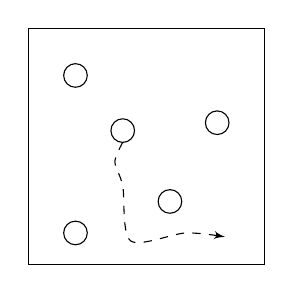
\begin{tikzpicture}
    \draw (0, 0) rectangle (3, 3);
    \draw (0.6, 0.4) circle [radius=0.15];
    \draw (1.8, 0.8) circle [radius=0.15];
    \draw (2.4, 1.8) circle [radius=0.15];
    \draw (0.6, 2.4) circle [radius=0.15];
    \draw (1.2, 1.7) circle [radius=0.15];
    \draw [-latex', dashed] plot [smooth] coordinates {(1.2, 1.55) (1.1, 1.3) (1.2, 1) (1.3, 0.3) (2, 0.4) (2.5, 0.35)};
  \end{tikzpicture}
\end{center}
In this regime, the colloid particles undergo Brownian motion. The time scale of the motion is determined by the diffusivity constant, which turns out to be
\[
  D = \frac{k_B T}{6 \pi \eta_s a},
\]
where $\eta_s$ is the solvent viscosity. Thus, the time $\tau$ it takes for the particle to move through a distance of its own radius $a$ is given by $a^2 = D \tau$, which we can solve to give
\[
  \tau \sim \frac{a^3 \eta_s}{ k_B T}.
\]
In general, this is much longer than the time scale $\tau_Q$ of quantum fluctuations, since $a^3 \eta_S \gg \hbar$.

When $\Phi > 0.55$, then the colloids fall into a crystal structure:
\begin{center}
  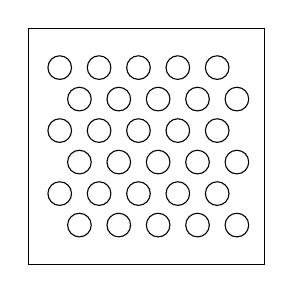
\begin{tikzpicture}
    \draw (-0.05, -0.1) rectangle +(3, 3);

    \draw (0.6, 0.4) circle [radius=0.15];
    \draw (1.1, 0.4) circle [radius=0.15];
    \draw (1.6, 0.4) circle [radius=0.15];
    \draw (2.1, 0.4) circle [radius=0.15];
    \draw (2.6, 0.4) circle [radius=0.15];

    \draw (0.35, 0.8) circle [radius=0.15];
    \draw (0.85, 0.8) circle [radius=0.15];
    \draw (1.35, 0.8) circle [radius=0.15];
    \draw (1.85, 0.8) circle [radius=0.15];
    \draw (2.35, 0.8) circle [radius=0.15];

    \draw (0.6, 1.2) circle [radius=0.15];
    \draw (1.1, 1.2) circle [radius=0.15];
    \draw (1.6, 1.2) circle [radius=0.15];
    \draw (2.1, 1.2) circle [radius=0.15];
    \draw (2.6, 1.2) circle [radius=0.15];

    \draw (0.35, 1.6) circle [radius=0.15];
    \draw (0.85, 1.6) circle [radius=0.15];
    \draw (1.35, 1.6) circle [radius=0.15];
    \draw (1.85, 1.6) circle [radius=0.15];
    \draw (2.35, 1.6) circle [radius=0.15];

    \draw (0.6, 2.0) circle [radius=0.15];
    \draw (1.1, 2.0) circle [radius=0.15];
    \draw (1.6, 2.0) circle [radius=0.15];
    \draw (2.1, 2.0) circle [radius=0.15];
    \draw (2.6, 2.0) circle [radius=0.15];

    \draw (0.35, 2.4) circle [radius=0.15];
    \draw (0.85, 2.4) circle [radius=0.15];
    \draw (1.35, 2.4) circle [radius=0.15];
    \draw (1.85, 2.4) circle [radius=0.15];
    \draw (2.35, 2.4) circle [radius=0.15];
  \end{tikzpicture}
\end{center}

Here the colloids don't necessarily touch, but there is still resistance to change in shape due to the entropy changes associated. We can find that the elasticity is given by
\[
  G \simeq k_B T \frac{N}{V}.
\]
%In the small $\Phi$ case, the ``source'' of entropy is clear, given by the disorder in the position of the colloids. Here the entropy is given by the ``rattle room'' entropy.

In both cases, we see that the elasticity and time scales are given in terms of $k_B T$. If we ignore thermal fluctuations, then we have $G = 0$ and $\tau = \infty$, which is extremely boring, and more importantly, is not how the real world behaves!

\subsection{The mathematics}
To model the systems, one might begin by looking at the microscopic laws of physics, and build models out of them. However, this is usually infeasible, because there are too many atoms and molecules lying around to track them individually. The solution is to do some \term{coarse-graining} of the system. For example, if we are modelling colloids, we can introduce a function $\psi(\mathbf{r})$ that tells us the colloid density near the point $\mathbf{r}$. We then look for laws on how this function $\psi$ behave, which is usually phenomenological, i.e.\ we try to find some equations that happen to model the real world well, as opposed to deriving these laws from the underlying microscopic principles. In general, $\psi$ will be some sort of \term{order parameter} that describes the substance.

The first thing we want to understand is the equilibrium statistical physics. This tell us what we expect the field $\psi$ to look like after it settles down, and also crucially, how the field is expected to fluctuate in equilibrium. Ultimately, what we get out of this is $P[\psi(r)]$, the probability (density) of seeing a particular field configuration at equilibrium. The simplest way of understanding this is via mean field theory, which seeks a single field $\psi$ that maximizes $P[\psi(r)]$. However, this does not take into account fluctuations, A slightly more robust way of dealing with fluctuations is the variational method, which we will study next.

After understanding the equilibrium statistical physics, we turn to understanding the dynamics, namely what happens when we start our system in a non-equilibrium state. We will be interested in systems that undergo phase transition. For example, liquid crystals tend to be in a disordered state at high temperatures and ordered at low temperatures. What we can do is then to prepare our liquid crystals at high temperature so that it stays at a homogeneous, disordered state, and then rapidly decrease the temperature. We then expect the system to evolve towards a ordered state, and we want to understand how it does so.

The first step to understanding dynamics is to talk about the hydrodynamic level equations, which are deterministic PDEs for how the system evolves. These usually look like
\[
  \dot{\psi}(\mathbf{r}, t) = \cdots,
\]
These equations come from our understanding of equilibrium statistical mechanics, and in particular that of the free energy functional and chemical potential. Naturally, the hydrodynamic equations do not take into account fluctuations, but report the expected evolution in time. These equations are particularly useful in late time behaviour where the existing movement and changes dominate over the small fluctuations.

To factor in the fluctuations, we promote our hydrodynamic PDEs to stochastic PDEs of the form
\[
  \dot{\psi}(\mathbf{r}, t) = \cdots + \text{noise}.
\]
Usually, the noise comes from random external influence we do not wish to explicitly model. For example, suspensions in water are bombarded by the water molecules all the time, and we model the effect by a noise term. Since the noise is the contribution of a large number of largely independent factors, it is reasonable to model it as Gaussian noise.

The mean noise will always be zero, and we must determine the variance. The key insight is that this random noise is the \emph{mechanism} by which the Boltzmann distribution arises. Thus, the probability distribution of the field $\psi$ determined by the stochastic PDE at equilibrium must coincide with what we know from equilibrium statistical dynamics. Since there is only one parameter we can toggle for the random noise, this determines it completely. This is the \emph{fluctuation dissipation theorem}.

%There are two parts to the study of soft condensed matters, confusingly and classically called \term{statics} and \term{dynamics}. The basic structure of the static part is going to look like this: we have some microscopic physics, but we don't want to track atoms and molecules. So we try to find some coarse-graining of the system. Thus, we come up with \emph{order parameter} fields, which we shall generically call $\psi(r)$. This goes into equilibrium statistical physics. To do this, we need to feed in symmetries and conservation laws. The output of this is some Boltzmann-distribution like probabilities $P[\psi(r)]$. In statistical physical field theory, $\psi$ might be our magnetization.
%
%To do dynamics, we want to think of $\psi(r)$ as a function of space and time. The starting point is ``hydrodynamic'' PDEs of the form
%\[
%  \dot{\psi}(r, t) = \cdots,
%\]
%and the thing on the right hand side will depend on the type of substance we are talking about, and this is often informed by the static equilibrium statistical physics. The next step to realize is that even in dynamics, we cannot forget about thermal fluctuations. However, the PDE itself is deterministic. Thus, we have to promote these to stochastic PDEs, which are of the form
%\[
%  \dot{\psi}(r, t) = \cdots + \text{noise}.
%\]
%This is informed by the static probability given by the fluctuation dissipation theorem, which fixes the noise by requiring that it produces the right equilibrium statistics. If we have a stochastic equation like this, the basic thing we are trying to find out is the probability $\P[\psi(r, t)]$ of a certain evolution of a system, not only in space but also in time.
%
%\begin{center}
%  \begin{tikzpicture}[xscale=4, yscale=2]
%    \node at (0, 0) {\textbf{statics}};
%    \node at (1, 0) {\textbf{dynamics}};
%    \node (mic) at (-1, -1) {microscopics};
%    \node (coarse) at (0, -1) {coarse-graining $\psi$};
%    \node (pde) at (1, -1) {hydrodynamic PDE};
%    \node (sym) [align=center] at (-1, -2) {symmetries and\\ conservation laws};
%    \node (equil) [align=center] at (0, -2) {equilibrium\\statistical physics};
%    \node (stochastic) at (1, -2) {stochastic PDE};
%    \node at (-1, -3) {probabilities};
%    \node (p1) at (0, -3) {$P[\psi(r)]$};
%    \node (p2) at (1, -3) {$\P[\psi(r, t)]$};
%
%    \draw [->] (mic) -- (coarse);
%    \draw [->] (sym) -- (equil);
%    \draw [->] (coarse) -- (equil);
%    \draw [->] (equil) -- (p1);
%    \draw [->] (coarse) -- (pde);
%    \draw [->] (pde) -- (stochastic);
%    \draw [->] (equil) -- (pde);
%    \draw [->] (p1) -- (stochastic) node [pos=0.5, anchor=north west] {FDT};
%    \draw [->] (stochastic) -- (p2);
%  \end{tikzpicture}
%\end{center}

\begin{eg}
  To model a one-component isothermal fluid such as water, we can take $\psi(\mathbf{r}, t)$ to consist of the density $\rho$ and velocity $\mathbf{v}$. The hydrodynamic PDE is exactly the \term{Navier--Stokes equation}. Assuming incompressibility, so that $\dot{\rho} = 0$, we get
  \[
    \rho (\dot{\mathbf{v}} + \mathbf{v} \cdot \nabla \mathbf{v}) = \eta \nabla^2 \mathbf{v} - \nabla p,
  \]
  We can promote this to a stochastic PDE, which is usually called the \term{Navier--Stokes--Landau--Lipschitz equation}. This is given by
  \[
    \rho (\dot{\mathbf{v}} + \mathbf{v} \cdot \nabla \mathbf{v}) = \eta \nabla^2 \mathbf{v} - \nabla p + \nabla \cdot \Sigma^N,
  \]
  The last term is thought of as a noise stress tensor on our fluid, and is conventionally treated as a Gaussian. As mentioned, this is fixed by the fluctuation-dissipation theorem, and it turns out this is given by
  \[
    \bra \Sigma_{ij}^N(r, t) \Sigma_{k \ell}^N (r', t')\ket = 2k_B T \eta (\delta_{i\ell} \delta_{jk} + \delta_{ik} \delta_{j\ell}) \delta(\mathbf{r} - \mathbf{r}') \delta(t - t').
  \]
\end{eg}

\begin{eg}
  If we want to describe a binary fluid, i.e.\ a mixture of two fluids, we introduce a further composition function $\phi$ that describes the (local) proportion of the fluids present.

  If we think about liquid crystals, then we need to add the molecular orientation.
\end{eg}

\section{Revision of equilibrium statistical physics}
\subsection{Thermodynamics}
A central concept in statistical physics is entropy.

\begin{defi}[Entropy]\index{entropy}
  The \emph{entropy} of a system is
  \[
    S = - k_B \sum_i p_i \log p_i,
  \]
  where $k_B$ is \term{Boltzmann's constant}, $i$ is a \term{microstate} --- a complete specification of the microscopics (e.g.\ the list of all particle coordinates and velocities) --- and $p_i$ is the probability of being in a certain microstate.
\end{defi}

The axiom of Gibbs is that a system in thermal equilibrium maximizes $S$ subject to applicable constraints.
\begin{eg}
  In an isolated system, the number of particles $N$, the energy $E$ and the volume $V$ are all fixed. Our microstates then range over all microstates that have this prescribed number of particles, energy and volume only. After restricting to such states, the only constraint is
  \[
    \sum_i p_i = 1.
  \]
  Gibbs says we should maximize $S$. Writing $\lambda$ for the Lagrange multiplier maintaining this constraint, we require
  \[
    \frac{\partial}{\partial p_i} \left(S - \lambda \sum_i p_i\right) = 0.
  \]
  So we find that
  \[
    -k_B \log p_i + 1 - \lambda = 0
  \]
  for all $i$. Thus, we see that all $p_i$ are equal.
\end{eg}
The above example does not give rise to the Boltzmann distribution, since our system is completely isolated. In the Boltzmann distribution, instead of fixing $E$, we fix the average value of $E$ instead.

\begin{eg}
  Consider a system of fixed $N, V$ in contact with a heat bath. So $E$ is no longer fixed, and fluctuates around some average $\bra E \ket = \bar{E}$. So we can apply Gibbs' principle again, where we now sum over all states of all $E$, with the restrictions
  \[
    \sum p_i E_i = \bar{E},\quad \sum p_i = 1.
  \]
  So our equation is
  \[
    \frac{\partial}{\partial p_i} \left(S - \lambda_I \sum p_i - \lambda_E \sum p_i E_i\right) = 0.
  \]
  Differentiating this with respect to $p_i$, we get
  \[
     -k_B (\log p_i + 1) - \lambda_I - \lambda_E E_i = 0.
  \]
  So it follows that
  \[
    p_i = \frac{1}{Z} e^{-\beta E_i},
  \]
  where $Z = \sum_i e^{-\beta E_i}$ and $\beta = \lambda_E/k_B$. This is the \term{Boltzmann distribution}.

  What is this mysterious $\beta$? Recall that the Lagrange multiplier $\lambda_E$ measures how $S$ reacts to a change in $\bar{E}$. In other words,
   \[
    \frac{\partial S}{\partial E} = \lambda_E = k_B \beta.
  \]
  Moreover, \emph{by definition} of temperature\index{temperature}, we have
  \[
    \left.\frac{\partial S}{\partial E}\right|_{V, N, \ldots} = \frac{1}{T}.
  \]
  So it follows that
  \[
    \beta = \frac{1}{k_B T}.
  \]
\end{eg}

Recall that the first law of thermodynamics says
\[
  \d E = T\;\d S - P \;\d V + \mu \;\d N + \cdots.
\]
This is a natural object to deal with when we have fixed $S, V, N$, etc. However, often, it is temperature that is fixed, and it is more natural to consider the free energy:
\begin{defi}[Helmholtz free energy]\index{Helmholtz free energy}
  The \emph{Helmholtz free energy} of a system at fixed temperature, volume and particle number is defined by
  \[
    F(T, V, N) = U - TS = \bar{E} - TS = - k_B T \log Z.
  \]
\end{defi}
This satisfies
\[
  \d F = -S \;\d T - P\;\d V + \mu\;\d N + \cdots,
\]
and is minimized at equilibrium for fixed $T, V, N$. % The derivative of $F$ in an isothermal system tells us ``which way it moves''.

\subsection{Coarse Graining}
Usually, in statistical mechanics, we distinguish between two types of objects --- microstates, namely the exact configuration of the system, and macrostates, which are variables that describe the overall behaviour of the system, such that pressure and temperature. Here we would like to consider something in between.

For example, if we have a system of magnets as in the Ising model, we the microstate would be the magnetization at each site, and the macrostate would be the overall magnetization. A coarse-graining of this would be a function $m(\mathbf{r})$ of space that describes the ``average magnetization around $\mathbf{r}$''. There is no fixed prescription on how large an area we average over, and usually it does not matter much.

In general, the coarse-grained variable would be called $\psi$. We can define a coarse-grained partition function
\[
  Z[\psi(\mathbf{r})] = \sum_{i \in \psi} e^{-\beta E_i},
\]
where we sum over all states that coarse-grain to $\psi$. We can similarly define the energy and entropy by restricting to all such $\psi$, and get
\[
  F[\psi] = E[\psi] - T S[\psi].
\]
The probability of being in a state $\psi$ is then
\[
  \P[\psi] = \frac{e^{-\beta F[\psi]}}{Z_{\mathrm{TOT}}},\quad Z_{\mathrm{TOT}} = \int e^{-\beta F[\psi]} \;\D [\psi].
\]
What we have on the end is a \emph{functional integral}, where we integrate over all possible values of $\psi$. We shall go into details later. We then have
\[
  F_{\mathrm{TOT}} = -k_B T \log Z_{\mathrm{TOT}}.
\]
In theory, one can obtain $F[\psi]$ by explicitly doing a coarse graining of the macroscopic laws.

\begin{eg}
  Consider an interacting gas with $N$ particles. We can think of the energy as a sum of two components, the ideal gas part ($\frac{d}{2}NkT$), and an interaction part, given by
  \[
    E_{\mathrm{int}} = \frac{1}{2}\sum_{i \not j} U(\mathbf{r}_i - \mathbf{r}_j),
  \]
  where $i, j$ range over all particles with positions $\mathbf{r}_i, \mathbf{r}_j$ respectively, and $U$ is some potential function. When we do coarse-graining, we introduce a function $\rho$ that describes the local density of particles. The interaction energy can then be written as
  \[
    E_{\mathrm{int}} = \frac{1}{2} \iint U(\mathbf{r} - \mathbf{r}') \rho(\mathbf{r}) \rho(\mathbf{r}') \;\d \mathbf{r} \;\d \mathbf{r}'.
  \]
  Similarly, up to a constant, we can write the entropy as
  \[
    S[\rho] = -k_B \int \rho(\mathbf{r}) \log \rho(\mathbf{r}) \;\d \mathbf{r}.
  \]
\end{eg}

In practice, since the microscopic laws aren't always accessible anyway, what is more common is to take a phenomenological approach, namely we write down a Taylor expansion of $F[\psi]$, and then empirically figure out what the coefficients should be, as a function of temperature and other parameters. In many cases, the signs of the first few coefficients dictate the overall behaviour of the system, and phase transition occurs when the change in temperature causes the coefficients to switch signs.

\section{Mean field theory}
In this chapter, we explore the mean field theory of two physical systems --- binary fluids and nematic liquid crystals. In mean field theory, what we do is we write down the free energy of the system, and then find a state $\phi$ that minimizes the free energy. By the Boltzmann distribution, this would be the ``most likely state'' of the system, and we can pretend $F_{\mathrm{TOT}} = F[\phi]$.

This is actually not a very robust system, since it ignores all the fluctuations about the minimum, but gives a good starting point for understanding the system.

\subsection{Binary fluids}
Consider a binary fluid, consisting of a mixture of two fluids $A$ and $B$. For simplicity, we assume we are in the symmetric case, where $A$ and $B$ are the same ``type'' of fluids. In other words, the potentials between the fluids are such that
\[
  U_{AA}(\mathbf{r}) = U_{BB}(\mathbf{r}) \not= U_{AB}(\mathbf{r}).
\]
We consider the case where $A$ and $B$ repulse each other (or rather, repulse each other more than the $A$-$A$ and $B$-$B$ repulsions). Thus, we expect that at high temperatures, entropy dominates, and the two fluids are mixed together well. At low temperatures, energy dominates, and the two fluids would be well-separated.

We let $\rho_A(\mathbf{r})$ and $\rho_B(\mathbf{r})$ be the coarse-grained particle density of each fluid, and we set our order parameter to be
\[
  \phi(\mathbf{r}) = \frac{\rho_A(\mathbf{r}) - \rho_B(\mathbf{r})}{(N_A + N_B)/V},
\]
with $N_A$ and $N_B$, the total amount of fluids $A$ and $B$, and $V$ the volume. This is normalized so that $\phi(\mathbf{r}) \in [-1, 1]$.

We model our system with \term{Landau--Ginzburg theory}, with free energy given by
\[
  \beta F = \int \Big(\underbrace{\frac{a}{2} \phi^2 + \frac{b}{4} \phi^4}_{f(\phi)} + \frac{\kappa}{2} (\nabla \phi)^2\Big)\;\d \mathbf{r},
\]
where $a, b, \kappa$ are functions of temperature.

Why did we pick such a model? Symmetry suggests the free energy should be even, and if we Taylor expand any even free energy functional, the first few terms will be of this form. For small $\phi$ and certain values of $a, b, \kappa$, we shall see there is no need to look further into higher order terms.

Observe that even without symmetry, we can always assume we do not have a linear term, since a $c \phi$ term will integrate out to give $cV \bar{\phi}$, and $\bar{\phi}$, the average composition of the fluid, is a fixed number. So this just leads to a constant shift.

The role of the gradient term $\int \frac{\kappa}{2} (\nabla \phi)^2 \;\d \mathbf{r}$ captures at order $\nabla^{(2)}$ the non-locality of $E_{int}$,
\[
  E_{\mathrm{int}} = \sum_{i, j \in \{A, B\}} \int \rho_i (\mathbf{r}) \rho_j(\mathbf{r}') U_{ij}(|\mathbf{r} - \mathbf{r}'|)\;\d \mathbf{r}\;\d \mathbf{r}',
\]
If we assume $\phi(\mathbf{r})$ is slowly varying on the scale of interactions, then we can Taylor expand this $E_{\mathrm{int}}$ and obtain a $(\nabla \phi)^2$ term.

Now what are the coefficients $a, b, \kappa$? For the model to make sense, we want the free energy to be suppressed for large fluctuating $\phi$. Thus, we want $b, \kappa > 0$, while $a$ can take either sign. In general, the sign of $a$ is what determines the behaviour of the system, so for simplicity, we suppose $b$ and $\kappa$ are fixed, and let $a$ vary with temperature.

To do mean field theory, we find a single $\phi$ that minimizes $F$. Since the gradient term $\int \frac{\kappa}{2} (\nabla \phi)^2\;\d x \geq 0$, a naive guess would be that we should pick a uniform $\phi$,
\[
  \phi(\mathbf{r}) = \bar{\phi}.
\]
Note that $\bar{\phi}$ is fixed by the constraint of the system, namely how much fluid of each type we have. So we do not have any choice. In this configuration, the free energy per unit volume is
\[
  \frac{F}{V} = f(\bar{\phi}) = \frac{a}{2} \bar{\phi}^2 + \frac{b}{4} \bar{\phi}^4.
\]
The global of this function depends only on the sign of $a$. For $a > 0$ and $a < 0$ respectively, the plots look like this:
\begin{center}
  \begin{tikzpicture}
    \draw [->] (-2.3, 0) -- (2.3, 0) node [right] {$\bar{\phi}$};
    \draw [->] (0, -1) -- (0, 3) node [above] {$f$};
    \draw [domain=-2:2, mblue, thick] plot (\x, {(\x)^2/3 + (\x)^4/10});
    \draw [domain=-2:2, mred, thick] plot [smooth] (\x, {-(\x)^2 + (\x)^4/3});

    \node [right, mblue] at (1.8, 2.13) {$a > 0$};
    \node [right, mred] at (1.9, 0.734) {$a < 0$};
    \node [left, white] at (-1.8, 2.13) {$a > 0$};
    \node [left, white] at (-1.9, 0.734) {$a < 0$};
  \end{tikzpicture}
\end{center}
We first think about the $a > 0$ part. The key point is that the function $f(\phi)$ is a convex function. Thus, for a fixed average value of $\phi$, the way to minimize $f(\phi)$ is to take $\phi$ to be constant. Thus, since
\[
  \beta F = \int \left(f(\phi(\mathbf{r})) + \frac{\kappa}{2} (\nabla \phi)^2\right)\;\d \mathbf{r},
\]
even considering the first term alone tells us we must take $\phi$ to be constant, and the gradient term reinforces this further.

The $a < 0$ case is more interesting. The function $f(\phi)$ has two minima, $\phi_{1, 2} = \pm \phi_B$, where
\[
  \phi_B = \sqrt{\frac{-a}{b}}.
\]
Now suppose $\bar{\phi}$ lies between $\pm \phi_B$. Then it might be advantageous to have some parts of the fluid being at $-\phi_B$ and the others at $\phi_B$, and join them smoothly in between to control the gradient term. Mathematically, this is due to the concavity of the function $f$ in the region $[-\phi_B, \phi_B]$.

Suppose there is $V_1$ many fluid with $\phi = \phi_1$, and $V_2$ many fluid with $\phi = \phi_2$. Then these quantities must obey
\begin{align*}
  V_1 \phi_1 + V_2 \phi_2 &= V \bar{\phi},\\
  V_1 + V_2 &= V.
\end{align*}
Concavity tells us we must have
\[
  V_1 f(\phi_1) + V_2 f(\phi_2) < (V_1 + V_2) f(\bar{\phi}).
\]
Thus, if we only consider the $f$ part of the free energy, it is advantageous to have this phase separated state. If our system is very large in size, since the interface between the two regions is concentrated in a surface of finite thickness, the gradient cost will be small compared to the gain due to phase separation.

We can be a bit more precise about the effects of the interface. In the first example sheet, we will explicitly solve for the actual minimizer of the free energy subject to the boundary condition $\phi(x) \to \pm \phi_B$ as $x \to \pm \infty$, as in our above scenario. We then find that the thickness of the interface is (of the order)
\[
  \xi_0 = \frac{-2 \kappa}{a},
\]
and the cost per unit area of this interface is
\[
  \sigma = \left(\frac{-8 \kappa a^3}{9 b^2}\right)^{1/2}.
\]
This is known as the \term{interfacial tension}. When calculating the free energy of a phase separated state, we will just multiply the interfacial tension by the area, instead of going back to explicit free energy calculations.

In general the mean-field phase diagram looks like
\begin{center}
  \begin{tikzpicture}
    \draw (-2, 3) node [above] {$a$} -- (-2, 0) node [below] {$-1$} -- (2, 0) node [below] {$1$} node [right] {$\bar \phi$} -- (2, 3);
    \node [left] at (-2, 2.5) {$a(T) = 0$};

    \draw [domain=2.5:0.2, samples=40, mblue, semithick] plot [smooth] ({sqrt (2.5 - \x)}, \x);
    \draw [domain=2.5:0.2, samples=40, mblue, semithick] plot [smooth] ({-sqrt (2.5 - \x)}, \x);

    \draw [dashed, domain=0.2:2.5, mred, semithick] plot [smooth] ({sqrt ((2.5 - \x)/3)}, \x);
    \draw [dashed, domain=0.2:2.5, mred, semithick] plot [smooth] ({-sqrt ((2.5 - \x)/3)}, \x);
    \draw (-2.05, 2.5) -- (-1.95, 2.5);
  \end{tikzpicture}
\end{center}
Within the solid lines, we have phase separation, where the ground state of the system for the given $a$ and $\bar{\phi}$ is given by the state described above. The inner curve denotes \term{spinodal instability}, where we in fact have local instability, as opposed to global instability. This is given by the condition $f''(\bar{\phi}) < 0$, which we solve to be
\[
  \phi_S = \sqrt{\frac{-a}{3b}}.
\]

What happens if our fluid is no longer symmetric? In this case, we should add odd terms as well. As we previously discussed, a linear term has no effect. How about a cubic term $\int \frac{c}{3} \phi(\mathbf{r})^3 \;\d \mathbf{r}$ to our $\beta F$? It turns out we can remove the $\phi(\mathbf{r})$ term by a linear shift of $\phi$ and $a$, which is a simple algebraic maneuver. So we have a shift of axes on the phase diagram, and nothing interesting really happens.

\subsection{Nematic liquid crystals}
For our purposes, we can imagine liquid crystals as being made of rod-like molecules
\begin{center}
  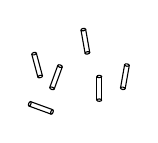
\begin{tikzpicture}[scale=0.3]
    \begin{scope}
      \draw (0, 1) ellipse (0.1 and 0.05);
      \draw (0, 0) ellipse (0.1 and 0.05);
      \draw (0.1, 0) -- (0.1, 1);
      \draw (-0.1, 0) -- (-0.1, 1);
    \end{scope}
    \begin{scope}[shift={(1, 0.5)},rotate=-10]
      \draw (0, 1) ellipse (0.1 and 0.05);
      \draw (0, 0) ellipse (0.1 and 0.05);
      \draw (0.1, 0) -- (0.1, 1);
      \draw (-0.1, 0) -- (-0.1, 1);
    \end{scope}
    \begin{scope}[shift={(-0.5, 2)},rotate=10]
      \draw (0, 1) ellipse (0.1 and 0.05);
      \draw (0, 0) ellipse (0.1 and 0.05);
      \draw (0.1, 0) -- (0.1, 1);
      \draw (-0.1, 0) -- (-0.1, 1);
    \end{scope}
    \begin{scope}[shift={(-2, -0.5)},rotate=70]
      \draw (0, 1) ellipse (0.1 and 0.05);
      \draw (0, 0) ellipse (0.1 and 0.05);
      \draw (0.1, 0) -- (0.1, 1);
      \draw (-0.1, 0) -- (-0.1, 1);
    \end{scope}
    \begin{scope}[shift={(-2, 0.5)},rotate=-20]
      \draw (0, 1) ellipse (0.1 and 0.05);
      \draw (0, 0) ellipse (0.1 and 0.05);
      \draw (0.1, 0) -- (0.1, 1);
      \draw (-0.1, 0) -- (-0.1, 1);
    \end{scope}
    \begin{scope}[shift={(-2.5, 1)},rotate=15]
      \draw (0, 1) ellipse (0.1 and 0.05);
      \draw (0, 0) ellipse (0.1 and 0.05);
      \draw (0.1, 0) -- (0.1, 1);
      \draw (-0.1, 0) -- (-0.1, 1);
    \end{scope}
  \end{tikzpicture}
\end{center}

We are interested in the transition between two phases:
\begin{itemize}
  \item The \term{isotropic phase}, where the rods are pointed in random directions.
  \item The \term{nematic phase}, where the rods all point in the same direction, so that there is a long-range orientation order, but there is no long range positional order.
\end{itemize}

In general, there can be two different sorts of liquid crystals --- the rods can either be symmetric in both ends or have ``direction''. Thus, in the first case, rotating the rod by $180^\circ$ does not change the configuration, and in the second case, it does. We shall focus on the first case in this section.

The first problem we have to solve is to pick an order parameter. We want to take the direction of the rod $\mathbf{n}$, but mod it out by the relation $\mathbf{n} \sim -\mathbf{n}$. One way to do so is to consider the second-rank traceless tensor $n_i n_j$. This has the property that $A_i n_i n_j$ is the component of a vector $\mathbf{A}$ in the direction of $\mathbf{n}$, and is invariant under $n_i \mapsto n_j$. Observe that if we normalize $\mathbf{n}$ to be a unit vector, then $n_i n_j$ has trace $1$. Thus, if we have isotropic rods in $d$ dimensions, then we have
\[
  \bra n_i n_j \ket = \frac{\delta_{ij}}{d}.
\]
In general, we can defined a coarse-grained order parameter to be
\[
  Q_{ij} (\mathbf{r}) = \bra n_i n_j\ket_{local} - \frac{1}{d} \delta_{ij}.
\]
This is then a traceless symmetric second-rank tensor that vanishes in the isotropic phase.

One main difference from the case of the binary fluid is that $Q_{ij}$ is no longer conserved., i.e.\ the ``total $Q$''
\[
  \int Q_{ij}(\mathbf{r})\;\d \mathbf{r}
\]
is not constant in time. This will have consequences for equilibrium statistical mechanics, but also the dynamics.

We now want to construct the leading-order terms of the ``most general'' free energy functional. We start with the local part $f(Q)$, which has to be a scalar built on $Q$. The possible terms are as follows:
\begin{enumerate}
  \item There is only one linear one, namely $Q_{ii} = \Tr(Q)$, but this vanishes.
  \item We can construct a quadratic term $Q_{ij} Q_{ji} = \Tr(Q^2)$, and this is in general non-zero.
  \item There is a cubic term $Q_{ij} Q_{jk} Q_{ki} = \Tr(Q^3)$, and is also in general non-zero.
  \item There are two possible quartic terms, namely $\Tr(Q^2)^2$ and $\Tr(Q^4)$.
\end{enumerate}
So we can write
\[
  f(Q) = a\Tr(Q^2) + c \Tr(Q^3) + b_1 \Tr(Q^2)^2 + b_2 \Tr(Q^4).
\]
This is the local part of the free energy up to fourth order in $Q$. We can go on, and in certain conditions we have to, but if these coefficients $b_i$ are sufficiently positive in an appropriate sense, this is enough.

How can we think about this functional? Observe that if all of the rods point tend to point in a fixed direction, say $z$, and are agnostic about the other two directions, then $Q$ will be given by
\[
  Q_{ij} =
  \begin{pmatrix}
    -\lambda/2 & 0 & 0\\
    0 & -\lambda/2 & 0\\
    0 & 0 & \lambda
  \end{pmatrix},\quad \lambda > 0.
\]
If the rod is agnostic about the $x$ and $y$ directions, but instead avoids the $z$-direction, then $Q_{ij}$ takes the same form but with $\lambda < 0$. For the purposes of $f(Q)$, we can locally diagonalize $Q$, and it should somewhat look like this form. So this seemingly-special case is actually quite general.

The $\lambda > 0$ and $\lambda < 0$ cases are physically very different scenarios, but the difference is only detected in the odd terms. Hence the cubic term is extremely important here. To see this more explicitly, we compute $f$ in terms of $\lambda$ as
\begin{align*}
  f(Q) &= a \left(\frac{3}{2} \lambda^2\right) + c \left(\frac{3}{4} \lambda^3\right) + b_1\left(\frac{9}{4} \lambda^4\right) + b_2 \left(\frac{9}{8} \lambda^4\right)\\
  &= \bar{a} \lambda^2 + \bar{c} \lambda^3 + \bar{b}\lambda^4.
\end{align*}
We can think of this in a way similar to the binary fluid, where $\lambda$ is are sole order parameter. We fix $\bar{b}$ and $\bar{c} < 0$, and then vary $\bar{a}$. In different situations, we get
\begin{center}
  \begin{tikzpicture}[yscale=4]
    \draw [->] (-1, 0) -- (4, 0) node [right] {$\lambda$};
    \draw [->] (0, -0.2) -- (0, 0.8) node [above] {$f$};
    \clip (-1, -0.16) rectangle (4.3, 0.8);
    \draw [domain=-1:4, samples=50, mred, semithick] plot [smooth] (\x, {(\x)^2/6 - (\x)^3/5 + (\x)^4 / 20});
    \draw [domain=-1:4, samples=50, mblue, semithick] plot [smooth] (\x, {(\x)^2/5 - (\x)^3/5 + (\x)^4 / 20});
    \draw [domain=-1:4, samples=50, mgreen, semithick] plot [smooth] (\x, {(\x)^2/3 - (\x)^3/5 + (\x)^4 / 20});

    \node [mgreen] at (1.3, 0.5) {\small$\alpha < \alpha_c$};
    \node [mblue] at (2.3, 0.35) {\small$\alpha = \alpha_c$};
    \node [mred] at (3.6, 0.2) {\small$\alpha > \alpha_c$};
  \end{tikzpicture}
\end{center}
Here the cubic term gives a discontinuous transition, which is a first-order transition. If we had $\bar{c} > 0$ instead, then the minima are on the other side.

We now move on to the gradient terms. The possible gradient terms up to order $\nabla^{(2)}$ and $Q^{(2)}$ are
\begin{align*}
  \kappa_1 \nabla_i \nabla_i Q_{j\ell} Q_{j\ell} &= \kappa_1 \nabla^2 \Tr(Q^2) \\
  \kappa_2 (\nabla_i Q_{im}) (\nabla_j Q_{jm}) &= \kappa_2(\nabla \cdot Q)^2\\
  \kappa_3 (\nabla_i Q_{jm}) (\nabla_j Q_{im}) &= \text{yuck}.
\end{align*}
Collectively, these three terms describe the energy costs of the following three things:
\begin{center}
  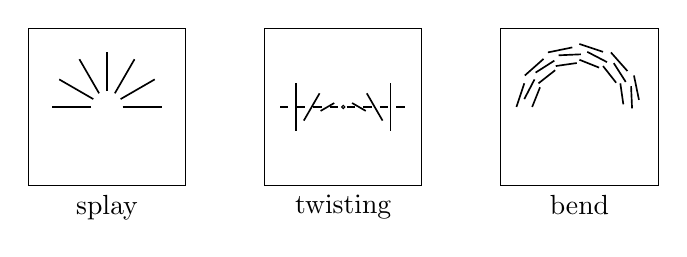
\begin{tikzpicture}
    \begin{scope}
      \draw (-1, -1) rectangle (1, 1);
      \node [below] at (0, -1) {splay};

      \draw [semithick] (0, 0.2) -- +(0, 0.5);
      \draw [semithick, rotate=30] (0, 0.2) -- +(0, 0.5);
      \draw [semithick, rotate=60] (0, 0.2) -- +(0, 0.5);
      \draw [semithick, rotate=90] (0, 0.2) -- +(0, 0.5);
      \draw [semithick, rotate=-30] (0, 0.2) -- +(0, 0.5);
      \draw [semithick, rotate=-60] (0, 0.2) -- +(0, 0.5);
      \draw [semithick, rotate=-90] (0, 0.2) -- +(0, 0.5);
    \end{scope}
    \begin{scope}[shift={(3, 0)}]
      \draw (-1, -1) rectangle (1, 1);
      \node [below] at (0, -1) {twisting};

      \draw [semithick] (-0.6, -0.3) -- +(0, 0.6);
      \draw [semithick] (0.6, -0.3) -- +(0, 0.6);

      \draw [semithick, rotate around={-30:(-0.4,0)}] (-0.4, -0.2) -- +(0, 0.4);
      \draw [semithick, rotate around={-60:(-0.2,0)}] (-0.2, -0.1) -- +(0, 0.2);

      \draw [semithick, rotate around={30:(0.4,0)}] (0.4, -0.2) -- +(0, 0.4);
      \draw [semithick, rotate around={60:(0.2,0)}] (0.2, -0.1) -- +(0, 0.2);

      \draw (0, 0) circle [radius=0.02];

      \draw [dashed, thin] (-0.8, 0) -- (0.8, 0);
    \end{scope}
    \begin{scope}[shift={(6, 0)}]
      \draw (-1, -1) rectangle (1, 1);
      \node [below] at (0, -1) {bend};

      \draw [semithick] (-0.8, 0) -- (-0.7, 0.3);
      \draw [semithick, rotate=-30] (-0.8, 0) -- (-0.7, 0.3);
      \draw [semithick, rotate=-60] (-0.8, 0) -- (-0.7, 0.3);
      \draw [semithick, rotate=-90] (-0.8, 0) -- (-0.7, 0.3);
      \draw [semithick, rotate=-120] (-0.8, 0) -- (-0.7, 0.3);
      \draw [semithick, rotate=-150] (-0.8, 0) -- (-0.7, 0.3);

      \draw [semithick] (-0.7, 0.1) -- (-0.57, 0.35);
      \draw [semithick, rotate=-30] (-0.7, 0.1) -- (-0.57, 0.35);
      \draw [semithick, rotate=-60] (-0.7, 0.1) -- (-0.57, 0.35);
      \draw [semithick, rotate=-90] (-0.7, 0.1) -- (-0.57, 0.35);
      \draw [semithick, rotate=-120] (-0.7, 0.1) -- (-0.57, 0.35);
      \draw [semithick, rotate=-150] (-0.7, 0.1) -- (-0.57, 0.35);

      \draw [semithick] (-0.6, 0) -- (-0.5, 0.25);
      \draw [semithick, rotate=-30] (-0.6, 0) -- (-0.5, 0.25);
      \draw [semithick, rotate=-60] (-0.6, 0) -- (-0.5, 0.25);
      \draw [semithick, rotate=-90] (-0.6, 0) -- (-0.5, 0.25);
      \draw [semithick, rotate=-120] (-0.6, 0) -- (-0.5, 0.25);
      \draw [semithick, rotate=-150] (-0.6, 0) -- (-0.5, 0.25);
    \end{scope}
  \end{tikzpicture}
\end{center}
In general, each of these modes correspond to linear combination of the three terms, and it is difficult to pin down how exactly these correspondences work.

Assuming these linear combinations are sufficiently generic, a sensible choice is to set $\kappa_1 = \kappa_3 = 0$ (for example), and then the elastic costs of these deformations will all be comparable.

\section{Functional derivatives and integrals}
We shall be concerned with two objects --- functional derivatives and integrals. Functional derivatives are (hopefully) familiar from variational calculus, and functional integrals might be something new. They will be central to what we are going to do next.

\subsection{Functional derivatives}
Consider a scalar field $\phi(\mathbf{r})$, and consider a functional
\[
  A[\phi] = \int L(\phi, \nabla \phi)\;\d \mathbf{r}.
\]
Under a small change $\phi \mapsto \phi + \delta \phi(\mathbf{r})$ with $\delta \phi = 0$ on the boundary, our functional becomes
\begin{align*}
  A[\phi + \delta \phi] &= \int \left(L(\phi, \nabla \phi) + \delta \phi \frac{\partial L}{\partial \phi} + \nabla d \phi \cdot \frac{\partial L}{\partial \phi}\right)\;\d \mathbf{r}\\
  &= A[\phi] + \int \delta \phi \left(\frac{\partial L}{\partial \phi} - \nabla \cdot \frac{\partial L}{\partial \nabla \phi}\right)\;\d \mathbf{r},
\end{align*}
where we integrated by parts using the boundary condition. This suggests the definition\index{functional derivative}\index{$\frac{\delta A}{\delta \phi(\mathbf{r})}$}
\[
  \frac{\delta A}{\delta \phi(\mathbf{r})} = \frac{\partial L}{\partial \phi(\mathbf{r})} - \nabla \cdot \frac{\partial L}{\partial \nabla \phi}.
\]
\begin{eg}
  In classical mechanics, we replace $\mathbf{r}$ by the single variable $t$, and $\phi$ by position $x$. We then have
  \[
    A = \int L(x, \dot{x})\;\d t.
  \]
  Then we have
  \[
    \frac{\delta A}{\delta x(t)} = \frac{\partial L}{\partial x} - \frac{\d}{\d t} \left(\frac{\partial L}{\partial \dot{x}}\right).
  \]
  The equations of classical mechanics are $\frac{\delta A}{\delta x(t)} = 0$.
\end{eg}

The example more relevant to us is perhaps Landau--Ginzburg theory:
\begin{eg}
  Consider a coarse-grained free energy
  \[
    F[\phi] = \int \left(\frac{a}{2} \phi^2 + \frac{b}{4} \phi^4 + \frac{\kappa}{2} (\nabla \phi)^2 \right)\;\d \mathbf{r}.
  \]
  Then
  \[
    \frac{\delta F}{\delta \phi(\mathbf{r})} = a \phi + b \phi^3 - \kappa \nabla^2 \phi.
  \]
  In mean field theory, we set this to zero, since by definition, we are choosing a single $\phi(\mathbf{r})$ that minimizes $F$. In the first example sheet, we find that the minimum is given by
  \[
    \phi(x) = \phi_B \tanh \left(\frac{x - x_0}{\xi_0}\right),
  \]
  where $\xi_0$ is the interface thickness we previously described.
\end{eg}

In general, we can think of $\frac{\delta F}{\delta \phi(\mathbf{r})}$ as a ``generalized force'', telling us how we should change $\phi$ to reduce the free energy, since for a small change $\delta \phi(\mathbf{r}))$, the corresponding change in $F$ is
\[
  \delta F = \int \frac{\delta F}{\delta \phi(\mathbf{r})} \;\delta \phi(\mathbf{r})\;\d \mathbf{r}.
\]
Compare this with the equation
\[
  \d F = - S \;\d T - p \;\d V + \mu \;\d N + \mathbf{h} \cdot \d \mathbf{M} + \cdots.
\]
Under the analogy, we can think of $\frac{\delta F}{\delta \phi(\mathbf{r})}$ as the intensive variable, and $\delta \phi(\mathbf{r})$ as the extensive variable. If $\phi$ is a conserved scalar density such as particle density, then we usually write this as
\[
  \mu(\mathbf{r}) = \frac{\delta F}{\delta \phi(\mathbf{r})},
\]
and call it the \term{chemical potential}. If instead $\phi$ is not conserved, e.g.\ the $Q$ we had before, then we write
\[
  H_{ij} = \frac{\delta F}{\delta Q_{ij}}
\]
and call it the \emph{molecular field}.

We will later see that in the case where $\phi$ is conserved, $\phi$ evolves according to the equation
\[
  \dot{\phi} = - \nabla \cdot J,\quad J \propto -D \nabla \mu,
\]
where $D$ is the diffusivity. The non-conserved case is simpler, with equation of motion given by.
\[
  \dot{Q} = - \Gamma H.
\]

Let us go back to the scalar field $\phi(\mathbf{r})$. Consider a small displacement
\[
  \mathbf{r} \mapsto \mathbf{r} + \mathbf{u}(\mathbf{r}).
\]
We take this to be incompressible, so that $\nabla \cdot \mathbf{u} = 0$. Then
\[
  \phi \mapsto \phi' = \phi'(\mathbf{r}) = \phi(\mathbf{r} - \mathbf{u}).
\]
Then
\[
  \delta \phi(\mathbf{r}) = \phi'(\mathbf{r}) - \phi(\mathbf{r}) = - \mathbf{u} \cdot \nabla \phi(\mathbf{r}) + O(u^2).
\]
Then
\begin{multline*}
  \delta F = \int \delta \phi \frac{\delta F}{\delta \phi}\;\d \mathbf{r}
  = -\int \mu \mathbf{u} \cdot \nabla \phi \;\d \mathbf{r}\\
  = \int \phi \nabla \cdot (\mu \mathbf{u})\;\d \mathbf{r}
  = \int (\phi \nabla \mu)\cdot \mathbf{u}\;\d \mathbf{r}
  = \int (\phi \nabla_j \mu)u_j\;\d \mathbf{r}.
\end{multline*}
using incompressibility.

We can think of the free energy change as the work done by stress,
\[
  \delta F = \int \sigma_{ij}(\mathbf{r}) \varepsilon_{ij}(\mathbf{r})\;\d \mathbf{r},
\]
where $\varepsilon_{ij} = \nabla_i u_j$ is the strain tensor, and $\sigma_{ij}$ is the stress tensor. So we can write this as
\[
  \delta F = \int \sigma_{ij} \nabla_i u_j\;\d \mathbf{r} = - \int (\nabla_i \sigma_{ij}) u_j\;\d \mathbf{r}.
\]
So we can identify
\[
  \nabla_i \sigma_{ij} = -\phi \nabla_j \mu.
\]
So $\mu$ also contains the ``mechanical information''.

\subsection{Functional integrals}
Given a coarse-grained $\psi$, we have can define the total partition function
\[
  e^{-\beta F_{\mathrm{TOT}}} = Z_{\mathrm{TOT}} = \int e^{-\beta F[\psi]} \;\D [\psi],
\]
where $\D [\psi]$ is the ``sum over all field configurations''. In mean field theory, we approximate this $F_{\mathrm{TOT}}$ by replacing the functional integral by the value of the integrand at its maximum, i.e.\ taking the minimum value of $F[\psi]$. What we are going to do now is to evaluate the functional integral ``honestly'', and this amounts to taking into account fluctuations around the minimum (since those far away from the minimum should contribute very little).

To make sense of the integral, we use the fact that the space of all $\psi$ has a countable orthonormal basis. We assume we work in $[0, L]^q$ of volume $V = L^q$ with periodic boundary conditions. We can define the Fourier modes
\[
  \psi_\mathbf{q} = \frac{1}{\sqrt{V}} \int \psi(\mathbf{r}) e^{-i\mathbf{q}\cdot \mathbf{r}}\;\d \mathbf{r},
\]
Since we have periodic boundary conditions, $\mathbf{q}$ can only take on a set of discrete values. Moreover, molecular physics or the nature of coarse-graining usually implies there is some ``maximum momentum'' $q_{max}$, above which the wavelengths are too short to make physical sense (e.g.\ vibrations in a lattice of atoms cannot have wavelengths shorter than the lattice spacing). Thus, we assume $\psi_\mathbf{q} = 0$ for $|\mathbf{q}| > q_{max}$. This leaves us with finitely many degrees of freedom.

The normalization of $\psi_\mathbf{q}$ is chosen so that \term{Parseval's theorem} holds:
\[
  \int |\psi|^2 \;\d \mathbf{r} = \sum_{\mathbf{q} } |\psi_\mathbf{q}|^2.
\]
We can then define
\[
  \D [\psi] = \prod_{\mathbf{q}} \;\d \psi_\mathbf{q}.
\]
Since we imposed a $q_{max}$, this is a finite product of measures, and is well-defined.

In some sense, $q_{max}$ is arbitrary, but for most cases, it doesn't really matter what $q_{max}$ we choose. Roughly speaking, at really short wavelengths, the behaviour of $\psi$ no longer depends on what actually is going on in the system, so these modes only give a constant shift to $F$, independent of interesting, macroscopic properties of the system. Thus, we will mostly leave the cutoff implicit, but it's existence is important to keep our sums convergent.

It is often the case that after doing calculations, we end up with some expression that sums over the $\mathbf{q}$'s. In such cases, it is convenient to take the limit $V \to \infty$ so that the sum becomes an integral, which is easier to evaluate.

An infinite product is still bad, but usually molecular physics or the nature of coarse graining imposes a maximum $q_{max}$, and we take the product up to there. In most of our calculations, we need such a $q_{max}$ to make sense of our integrals, and that will be left implicit. Most of the time, the results will be independent of $q_{max}$ (for example, it may give rise to a constant shift to $F$ that is independent of all the variables of interest).

Before we start computing, note that a significant notational annoyance is that if $\psi$ is a real variable, then $\psi_\mathbf{q}$ will still be complex in general, but they will not be independent. Instead, we always have
\[
  \psi_\mathbf{q} = \psi_{-\mathbf{q}}^*.
\]
Thus, we should only multiply over half of the possible $\mathbf{q}$'s, and we usually denote this by something like $\prod^+_{\mathbf{q}}$.

In practice, there is only one path integral we are able to compute, namely when $\beta F$ is a quadratic form, i.e.
\[
  \beta F = \frac{1}{2} \int \phi(\mathbf{r}) G(\mathbf{r} - \mathbf{r}') \phi(\mathbf{r}')\;\d \mathbf{r}\;\d \mathbf{r}' - \int h(\mathbf{r}) \phi(\mathbf{r})\;\d \mathbf{r}.
\]
Note that this expression is non-local, but has no gradient terms. We can think of the gradient terms we've had as localizations of first-order approximations to the non-local interactions. Taking the Fourier transform, we get
\[
  \beta F[\psi_\mathbf{q}] = \frac{1}{2} \sum_q G(\mathbf{q}) \phi_\mathbf{q} \phi_{-\mathbf{q}} - \sum_\mathbf{q} h_\mathbf{q} \phi_\mathbf{q}.
\]
\begin{eg}
  We take Landau--Ginzburg theory and consider terms of the form
  \[
    \beta F[\phi] = \int \left\{\xi \phi^2 - h \phi + \frac{\kappa}{2} (\nabla \phi)^2 + \frac{\gamma}{2} (\nabla^2 \phi)^2\right\}\;\d \mathbf{r}
  \]
  The $\gamma$ term is new, and is necessary because we will be interested in the case where $\kappa$ is negative.

  We can now take the Fourier transform to get
  \begin{align*}
    \beta F \{\phi_\mathbf{q}\} &= \frac{1}{2} \sum_\mathbf{q}\splus (a + \kappa q^2 + \gamma q^4) \phi_\mathbf{q} \phi_{-\mathbf{q}} - \sum_\mathbf{q}\splus h_\mathbf{q} \phi_\mathbf{q}.\\
    &= \sum_\mathbf{q}\splus (a + \kappa q^2 + \gamma q^4) \phi_\mathbf{q} \phi_{-\mathbf{q}} - \sum_\mathbf{q}\splus h_\mathbf{q} \phi_\mathbf{q}.
  \end{align*}
  So our $G(\mathbf{q})$ is given by
  \[
    G(\mathbf{q}) = a + k q^2 + \gamma q^4.
  \]
\end{eg}
To actually perform the functional integral, first note that if $h \not= 0$, then we can complete the square so that the $h$ term goes away. So we may assume $h = 0$. We then have
\begin{align*}
  Z_{\mathrm{TOT}} &= \int \left[ \prod_{\mathbf{q}}\splus \;\d \phi_\mathbf{q}\right] e^{-\beta F\{\phi_\mathbf{q}\}}\\
  &= \prod_\mathbf{q}\splus \int \d \phi_\mathbf{q}\;e^{-|\phi_\mathbf{q}|^2 G(q)}
\end{align*}
Each individual integral can be evaluated as
\[
  \int \d \phi_\mathbf{q}\;e^{-|\phi_\mathbf{q}|^2 G(q)} = \int \rho \;\d \rho \;\d \theta\; e^{-G(q) \rho^2} = \frac{\pi}{G(q)},
\]
where $\phi_\mathbf{q} = \rho e^{i\theta}$. So we find that
\[
  Z_{\mathrm{TOT}} = \prod_\mathbf{q}\splus \frac{\pi}{G(q)},
\]
and so
\[
  \beta F_T = -\log Z_T = \sum_\mathbf{q}\splus \log \frac{G(q)}{\pi}.
\]
We now take large $V$ limit, and replace the sum of the integral. Then we get
\[
  \beta F_T = \frac{1}{2} \frac{V}{(2\pi)^d} \int^{q_{max}} \d \mathbf{q}\;\log \frac{G(q)}{\pi}.
\]
There are many quantities we can compute from the free energy.
\begin{eg}
  The \term{structure factor} is defined to be
  \[
    S(\mathbf{k}) = \bra \phi_\mathbf{k} \phi_{-\mathbf{k}}\ket = \frac{1}{Z_T} \int \phi_\mathbf{k} \phi_{-\mathbf{k}} e^{-\sum_\mathbf{q}^+ \phi_\mathbf{q} \phi_{-\mathbf{q}} G(q)} \prod_q\splus \;\d \phi_\mathbf{q}.
  \]
  We see that this is equal to
  \[
    \frac{1}{Z_T} \frac{\partial Z_T}{\partial G(\mathbf{k})} = - \frac{\partial \log Z_T}{\partial G(\mathbf{k})} = \frac{1}{G(k)}.
  \]
  We could also have done this explicitly using the product expansion.

  This $S(k)$ is measured in scattering experiments. In our previous example, for small $k$ and $\kappa > 0$, we have
  \[
    S(q) = \frac{1}{a + \kappa k^2 + \gamma k^4} \approx \frac{a^{-1}}{1 + k^2 \xi^2},\quad
    \xi = \sqrt{\frac{\kappa}{a}}.
  \]
  where $\xi$ is the \term{correlation length}. We can return to real space by
  \begin{align*}
    \bra \phi^2(\mathbf{r})\ket &= \frac{1}{V} \left\bra \int |\phi(\mathbf{r})|^2 \;\d \mathbf{r}\right\ket \\
    &= \frac{1}{V} \sum_q \bra \phi_\mathbf{q}|^2\ket\\
    &= \frac{1}{(2\pi)^d} \int^{q_{max}} \frac{\d \mathbf{q}}{a + \kappa q^2 + \gamma q^4}.
  \end{align*}
\end{eg}

\section{The variational method}
\subsection{The variational method}
The variational method is a method to estimate the partition function
\[
  e^{-\beta F_{\mathrm{TOT}}} = \int e^{-\beta F[\phi]} \;\D [\phi]
\]
when $F$ is not Gaussian. To simplify notation, we will set $\beta = 1$. It is common to make a notational change, where we replace $F_{\mathrm{TOT}}$ with $F$ and $F[\phi]$ with $H[\phi]$. We then want to estimate
\[
  e^{-F_{\mathrm{TOT}}} = \int e^{-F[\phi]}\;\D [\phi].
\]
% What can we do when our free energy is not quadratic? What we previously did was to do mean field theory, but we know this fails near the critical point. In Statistical Field Theory, we used renormalization group methods. Here we go for something in between, namely the variational method. In condensed matter physics, this is known as \term{Hartree theory}, and in QFT it is known as ``\term{1-loop self consistency}''. This theory handles large Gaussian fluctuations well, and we shall use it to study smectic liquid crystals.
We now make a notation change, where we write $F_{\mathrm{TOT}}$ as $F$, and $F[\phi]$ as $H[\phi]$ instead, called \term{the effective Hamiltonian}. In this notation, we write
\[
  e^{-F} = \int e^{-H[\phi]} \;\D [\phi].
\]
The idea of the variational method is to find some upper bounds on $F$ in terms of path integrals we \emph{can} do, and then take the best upper bound as our approximation to $F$.

Thus, we introduce a \term{trial Hamiltonian} $H_0[\phi]$, and similarly define
\[
  e^{-F_0} = \int e^{-H_0[\phi]} \;\D [\phi].
\]
We can then write
\[
  e^{-F} = \frac{e^{-F_0}}{\int e^{-H_0}\;\D [\phi]} \int e^{-H_0} e^{-(H - H_0)}\;\D [\phi] = e^{-F_0} \bra e^{-(H - H_0)} \ket_0,
\]
where the subscript $0$ denotes the average over the trial distribution. Taking the logarithm, we end up with
\[
  F = F_0 - \log \bra e^{-(H - H_0)}\ket_0.
\]
So far, everything is exact. It would be nice if we can move the logarithm inside the expectation to cancel out the exponential. While the result won't be exactly equal, the fact that $\log$ is concave, i.e.
\[
  \log (\alpha A + (1 - \alpha) B) \geq \alpha \log A + (1 - \alpha) \log B.
\]
Thus Jensen's inequality tells us
\[
  \log \bra Y \ket_0 \geq \bra \log Y \ket_0.
\]
Applying this to our situation gives us an inequality
\[
  F \leq F_0 - \bra H_0 - H\ket_0 = F_0 - \bra H_0\ket_0 + \bra H\ket_0 = S_0 + \bra H\ket_0.
\]
This is the \term{Feynman--Bogoliubov inequality}.

To use this, we have to choose the trial distribution $H_0$ simple enough to actually do calculations (i.e.\ Gaussian), but include variational parameters in $H_0$. We then minimize the quantity $F_0 - \bra H_0\ket + \bra H\ket_0$ over our variational parameters, and this gives us an upper bound on $F$. We then take this to be our best estimate of $F$. If we are brave, we can take this minimizing $H_0$ as an approximation of $H$, at least for some purposes.

\subsection{Smectic liquid crystals}
We use this to talk about the isotropic to smectic transition in liquid crystals. The molecules involved often have two distinct segments. For example, we may have soap molecules that look like this:
\begin{center}
  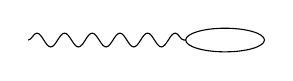
\begin{tikzpicture}
    \draw (3, 0) ellipse (0.5 and 0.15);
    \draw [decorate, decoration=snake] (0.5, 0) -- (2.5, 0);
  \end{tikzpicture}
\end{center}
The key property of soap molecules is that the tail hates water while the head likes water. So we expect these molecules to group together like
\begin{center}
  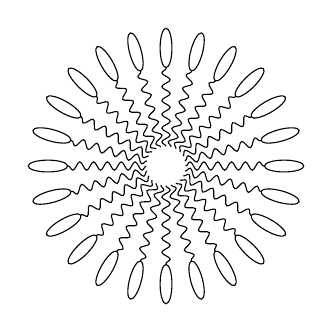
\begin{tikzpicture}[scale=0.5]
    \foreach \r in {0,15,...,345} {
      \begin{scope}[rotate=\r]
        \draw (3, 0) ellipse (0.5 and 0.15);
        \draw [decorate, decoration={snake, amplitude=1.5, segment length=5}] (0.5, 0) -- (2.5, 0);
      \end{scope}
  }
  \end{tikzpicture}
\end{center}
In general, we can imagine our molecules look like
\begin{center}
  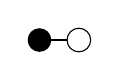
\begin{tikzpicture}[rotate=90, scale=0.5]
    \fill circle [radius=0.3];
    \draw (0, -1) circle [radius=0.3];
    \draw (0, -0.3) -- (0, -0.7);
  \end{tikzpicture}
\end{center}
and like attracts like. As in the binary fluid, we shall assume the two heads are symmetric, so $U_{AA} = U_{BB} \not= U_{AB}$. If we simply want the different parts to stay away from each other, then we can have a configuration that looks like
\begin{center}
  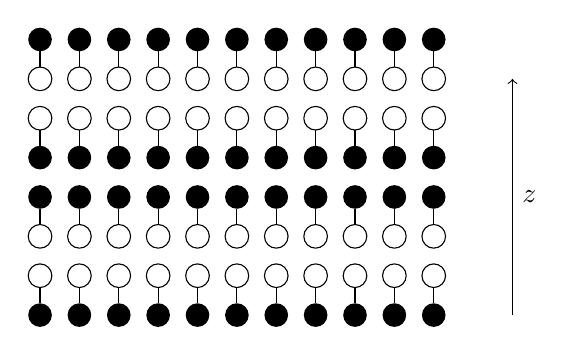
\begin{tikzpicture}[scale=0.5]
    \foreach \x in {0,...,10} {
      \foreach \y in {0,4} {
        \begin{scope}[shift={(\x, \y)}]
          \fill circle [radius=0.3];
          \draw (0, -1) circle [radius=0.3];
          \draw (0, -2) circle [radius=0.3];
          \fill (0, -3) circle [radius=0.3];
          \draw (0, -0.3) -- (0, -0.7);
          \draw (0, -2.3) -- (0, -2.7);
        \end{scope}
      }
   }
   \draw [->] (12, -3) -- (12, 3) node [pos=0.5, right] {$z$};
  \end{tikzpicture}
\end{center}
In general, we expect that there is such an order along the $z$ direction, as indicated, while there is no restriction on the alignments in the other directions. So the system is a lattice in the $z$ direction, and a fluid in the remaining two directions. This is known as a \term{smectic liquid crystal}, and is also known as the \term{lamellar phase}. This is an example of \term{microphase separation}.

As before, we let $\phi$ be a coarse grained relative density. The above ordered phase would then look like
\[
  \phi(\mathbf{x}) = \cos q_0 z.
\]
for some $q_0$ that comes from the molecular length. If our system is not perfectly ordered, then we may expect it to look roughly like $A \cos q_0 z$ for some $A$.

We again use Landau--Ginzburg model, which, in our old notation, has
\[
  \beta F = \int \left(\frac{a}{2} \phi^2 + \frac{b}{4} \phi^4 + \frac{\kappa}{2} (\nabla \phi)^2 + \frac{\gamma}{2} (\nabla^2 \phi)^2\right)\;\d \mathbf{r}.
\]
If we write this in Fourier space, then we get
\[
  \beta F = \frac{1}{2} \sum_{\mathbf{q}} (a + \kappa q^2 + \gamma q^4) \phi_{\mathbf{q}} \phi_{-\mathbf{q}} + \frac{b}{4V} \sum_{\mathbf{q}_1, \mathbf{q}_2, \mathbf{q}_3} \phi_{\mathbf{q}_1} \phi_{\mathbf{q}_2} \phi_{\mathbf{q}_3} \phi_{-(\mathbf{q}_1 + \mathbf{q}_2 + \mathbf{q}_3)}.
\]
Notice that the quartic term results in the rather messy sum at the end. For the iso-smectic transition, we choose $\kappa < 0, \gamma > 0$.

Again for simplicity, we first consider the case where $b = 0$. Then this is a Gaussian model with
\[
  G(q) = a + \kappa q^2 + \gamma q^4 = \tau + \alpha(q - q_0)^2,
\]
Varying $a$ gives a linear shift in $G(q)$. As we change $a$, we get multiple different curves.
\begin{center}
  \begin{tikzpicture}[xscale=3]
    \draw [->] (0, 0) -- (1.3, 0) node [right] {$q$};
    \draw [->] (0 ,0) -- (0, 3) node [above] {$G(q)$};

    \draw [domain=0:1.3] plot [smooth] (\x, {1 - \x^2 + \x^4});
    \draw [domain=0:1.3, thick, mred] plot [smooth] (\x, {0.25 - \x^2 + \x^4});
    \draw [domain=0:1.3] plot [smooth] (\x, {1.75 - \x^2 + \x^4});
    \node [right, mred] at (1.3, 1.4161) {$a = a_c$};

    \node [circ] at (0.707, 0) {};
    \node [below] at (0.707, 0) {$q_0$};
  \end{tikzpicture}
\end{center}
Thus, as $a$ decreases, $S(q) = \bra |\phi_\mathbf{q}|^2 \ket = \frac{1}{G(q)}$ blows up at some finite
\[
  q = q_0 = \sqrt{\frac{-\kappa}{2\gamma}},\quad a_c = \frac{\kappa^2}{4 \gamma}.
\]
We should take this blowing up as saying that the $|\mathbf{q}| = q_0$ states are highly desired, and this results in an ordered phase. Note that \emph{any} $\mathbf{q}$ with $|\mathbf{q}| = q_0$ is highly desired. When the system actually settles to an ordered state, it has to \emph{pick} one such $\mathbf{q}$ and let the system align in that direction. This is \term{spontaneous symmetry breaking}.

It is convenient to complete to square, and expand $G$ about $q = q_0$ and $a = a_c$. Then we have
\[
  G(q) = \tau + \alpha(q - q_0)^2,
\]
where
\[
  \tau = a - a_c,\quad \alpha = \frac{1}{2} G''(q_0) = - 2\kappa.
\]
Then the transition we saw above happens when $\tau = 0$.

We now put back the quartic term. We first do this with mean field theory, and then later return to the variational method.
\subsubsection*{Mean Field Theory}
In mean field theory, it is easier to work in real space. We look for a single field configuration that minimizes $F$. As suggested before, we try a solution of the form
\[
  \phi = A \cos q_0 z,
\]
which is smectic along $z$. We can then evaluate the free energy (per unit volume) to be
\[
  \frac{\beta F}{V} = \beta \overline{F[\phi]} = \frac{a}{2} \overline{\phi^2} + \frac{\kappa}{2} \overline{(\nabla \phi)^2} + \frac{\gamma}{2} \overline{(\nabla^2 \phi)^2} + \frac{b}{4} \overline{\phi^4}
\]
where the bar means we average over one period of the periodic structure. It is an exercise to directly compute
\[
  \overline{\phi^2} = \frac{1}{2} A^2,\quad \overline{(\nabla \phi)^2} = \frac{1}{2} A^2 q_0^2,\quad \overline{(\nabla^2 \phi)^2} =\frac{1}{2} A^2 q_0^4,\quad \overline{\phi^4} = \frac{3}{8} A^4.
\]
This gives
\[
  \frac{\beta F}{V} = \frac{1}{4} \left[aA^2 + \kappa A^2 q_0^2 + \gamma A^2 q_0^4 + \frac{3b}{8} A^4\right] = \frac{1}{4} \left[ A^2 \underbrace{(a - a_c)}_\tau + \frac{3b}{8} A^4\right].
\]
Note that $q_0$ is fixed by the system as we originally had, while $A$ is the amplitude of the fluctuation which we get to choose. Plotting this, we get a familiar graph
\begin{center}
  \begin{tikzpicture}
    \draw [->] (-2.3, 0) -- (2.3, 0) node [right] {$A$};
    \draw [->] (0, -1) -- (0, 3) node [above] {$\beta F/V$};
    \draw [domain=-2:2, mblue, thick] plot (\x, {(\x)^2/3 + (\x)^4/10});
    \draw [domain=-2:2, mred, thick] plot [smooth] (\x, {-(\x)^2 + (\x)^4/3});

    \node [right, mblue] at (1.8, 2.13) {$\tau > 0$};
    \node [right, mred] at (1.9, 0.734) {$\tau < 0$};
    \node [left, white] at (-1.8, 2.13) {$\tau > 0$};
    \node [left, white] at (-1.9, 0.734) {$\tau < 0$};
  \end{tikzpicture}
\end{center}
If $\tau > 0$, then the optimum solution is given by $A = 0$. Otherwise, we should pick $A \not= 0$. Observe that as we slowly reduce $\tau$ across $0$, the minimum varies \emph{continuously} with $\tau$:
\begin{center}
  \begin{tikzpicture}
    \draw [->] (0, 0) -- (4, 0) node [right] {$a$};
    \draw [->] (0, 0) -- (0, 3) node [above] {$|A|$};

    \draw [mblue, thick] (3.9, 0) -- (2, 0);
    \draw [domain=0:2, mblue, thick, samples=30] plot [smooth] (\x, {sqrt(2 - \x)});

    \node [below] at (2, 0) {$a_c$};
  \end{tikzpicture}
\end{center}
\subsubsection*{Variational method}
We now consider the variational theory. In the notation we were using previously, we have
\[
  H = \sum_\mathbf{q} \splus \phi_\mathbf{q} \phi_{-\mathbf{q}} G(q) + \frac{b}{4V} \sum_\mathbf{q} \phi_{\mathbf{q}_1} \phi_{\mathbf{q}_2} \phi_{\mathbf{q}_3} \phi_{-(\mathbf{q}_1 + \mathbf{q}_2 + \mathbf{q}_3)}.
\]
Our trial $H_0$ is
\[
  H_0 = \sum_\mathbf{q} \phi_\mathbf{q} \phi_{-\mathbf{q}} J(q).
\]
Since this is a Gaussian model, we know that
\[
  F_0 = \sum_{\mathbf{q}} \splus \log \frac{J(q)}{\pi}.
\]
To use our inequality, we need to evaluate our other two bits. We have
\[
  \bra H_0\ket_0 = \sum_{\mathbf{q}}\splus \bra \phi_\mathbf{q} \phi_{-\mathbf{q}}\ket_0 J(q).
\]
We already calculated
\[
  \bra \phi_{\mathbf{q}} \phi_{-\mathbf{q}} \ket_0 = \frac{1}{J(q)}.
\]
Thus, we have
\[
  \bra H_0 \ket_0 = \sum_{\mathbf{q}} \splus 1.
\]
Here it is clear that we must impose a cutoff on $\mathbf{q}$. We can think of this $1$ as the equipartition theorem.

We can also compute
\[
  \bra H\ket_0 = \sum_\mathbf{q} \splus \frac{1}{J(q)} G(q) + \frac{b}{4V} \underbrace{\sum_{\mathbf{q}_1, \mathbf{q}_2, \mathbf{q}_3}\bra \phi_{\mathbf{q}_1} \phi_{\mathbf{q}_2} \phi_{\mathbf{q}_3} \phi_{-(\mathbf{q}_1 \mathbf{q}_2 \mathbf{q}_3)}\ket_0}.
\]
In the Gaussian model, each $\phi_\mathbf{q}$ is a zero mean Gaussian random variables, which have certain nice properties. \term{Wick's theorem} tells us we have
\[
  \bra abcd \ket_0 = \bra ab\ket_0 \bra cd\ket_0 + \bra ac\ket_0 \bra bd\ket_0 + \bra ad\ket_0 \bra bc\ket_0.
\]
Applying this, together with the result
\[
  \bra \phi_{\mathbf{q}_1} \phi_{\mathbf{q}_0}\ket_0 = \bra |\phi_\mathbf{q}|^2 \ket_0 \delta_{\mathbf{q}_1, - \mathbf{q}_2},
\]
we obtain
\[
  U = 3 \left[\sum_\mathbf{q} \bra |\phi_\mathbf{q}|^2\ket_0\right]^2 = 12 \left[\sum_\mathbf{q} \splus \frac{1}{J(q)}\right]^2.
\]
Thus, we have
\[
  \bra H_0\ket_0 = \sum_{\mathbf{q}} \splus \frac{G(q)}{J(q)} + \frac{3b}{V} \left(\sum_\mathbf{q} \splus \frac{1}{J(q)}\right)^2.
\]
We can then compute
\[
  \tilde{F} = \sum_{\mathbf{q}} \splus \left(\log \frac{J(q)}{\pi} - 1 + \frac{G(q)}{J(q)}\right) + \frac{3b}{V}\left(\sum_\mathbf{q} \splus \frac{1}{J(q)}\right)^2.
\]
We minimize over $J(q)$ by solving
\[
  \frac{\partial \tilde{F}}{\partial J(q)} = 0
\]
for all $\mathbf{q}$. Differentiating, we obtain
\[
  \frac{1}{J(q)} - \frac{G(q)}{J(q)^2} - \frac{6b}{V J(q)^2} \sum_{\mathbf{q}'} \splus \frac{1}{J(q')} = 0.
\]
Multiplying through by $J^2$, we get
\[
  J(q) = G(q) + \frac{6b}{V} \sum_{\mathbf{q}'} \splus \frac{1}{J(q')}.
\]
For large $V$, we can replace the sum by an integral, and we have
\[
  J(q) = G(q) + \frac{3b}{(2\pi)^d} \int \frac{\d \mathbf{q}'}{J(\mathbf{q}')}.
\]
It is very important that once we have fixed $J(\mathbf{q})$, the second term is a constant. Writing
\[
  C = \frac{2}{V} \sum_{\mathbf{q}'} \splus \frac{1}{J(q')} = \frac{1}{(2\pi)^d} \int \frac{\d \mathbf{q}'}{J(\mathbf{q}')},
\]
we can then say the minimum is given by $J(q) = G(q) + 3bC$. Thus, solving for $J(q)$ is equivalent to finding a $C$ such that
\[
  C = \frac{1}{(2\pi)^d} \int \frac{\d \mathbf{q}'}{G(q) + 3bC}.
\]
This is a \term{self-consistency equation} for $C$ (and hence $J$).

There is a very concrete interpretation of $C$. Recall that $\bra \phi^2\ket$ is the average value of $\phi^2$ at some point $\mathbf{r}$ (which is independent of $\mathbf{r}$. So we can compute
\[
  \bra \phi(\mathbf{r})^2\ket = \frac{1}{V} \int \bra \phi(\mathbf{r})^2\ket \;\d \mathbf{r} = \frac{1}{V} \sum_q \bra |\phi_\mathbf{q}|^2 \ket = \frac{1}{V} \sum_{\mathbf{q}} \frac{1}{J(\mathbf{q})}.
\]
Thus, what our computation above amounts to is that we replaced $G(q)$ by $G(q) + 3b \bra \phi^2\ket$.

A good way to think about this is that we are approximating the $\phi^4$ term in the free energy by
\[
  \frac{b}{4} \phi^4 \approx \frac{3b}{2} \bra \phi^2\ket \phi^2.
\]
We have to pick a value so that this approximation is consistent. We view the $\bra \phi^2\ket$ above as just another constant, so that the free energy is now a Gaussian. We can compute the expectation of $\phi^2$ using this free energy, and then we find that
\[
  \bra \phi^2\ket = \frac{1}{(2\pi)^d} \int \frac{\d \mathbf{q}'}{G(q) + 3b \bra \phi^2\ket}.
\]
This is the self-consistency equation as above.

We could have done the approximation above without having to through the variational method, but the factor of $\frac{3b}{2}$ is then no longer obvious.

%The factor of $\frac{3b}{2}$ is motivated by the previous calculation. Using this, we then treat $\bra\phi^2\ket$ as a constant and do our path integral calculation as before. Note that in principle, $\bra \phi^2\ket$ is a function of position, namely the expected value of $\phi^2$ at position $\mathbf{r}$. But this, of course, does not depend on $\mathbf{r}$. So we have
%\[
%  \bra \phi^2\ket = \bra \phi(\mathbf{r})^2\ket = \frac{1}{V} \int \bra \phi(\mathbf{r})^2\ket \;\d \mathbf{r} = \frac{1}{V} \sum_q \bra |\phi_\mathbf{q}|^2 \ket = \frac{1}{V} \sum_{\mathbf{q}} \frac{1}{G(q) + \bra \phi^2\ket},
%\]
%where the last equality follows from our previous calculations. Finding a value of $\bra \phi^2\ket$ that makes this equation consistent is exactly the same as solving for $C$ above. This $C$ has a very concrete interpretation.
%Informally, there is another way of viewing these types of calculations. This is a self-consistent treatment of the quartic. This is equivalent to making the following ad hoc approximation inside the Landau--Ginzburg theory.
%\[
%  \int \left\{ \frac{a}{2} \phi^2 + \frac{b}{4} \phi^4\right\} \;\d \mathbf{r} \mapsto \int \left\{ \frac{a}{2} \phi^2 + \frac{3b}{2} \bra \phi^2 \ket \phi^2\right\}\;\d \mathbf{r}'
%\]
%While $\bra \phi^2\ket = \bra \phi(\mathbf{r})^2\ket$ is the average over all ensembles at a fixed point $\mathbf{r}$, it is equal to what we get by averaging over all points, so
%\[
%  \bra \phi(\mathbf{r})^2\ket = \frac{1}{V} \int \bra \phi(\mathbf{r})^2\ket \;\d \mathbf{r} = \frac{1}{V} \sum_q \bra |\phi_\mathbf{q}|^2 \ket = \frac{1}{V} \sum_{\mathbf{q}} \frac{1}{J(\mathbf{q})}.
%\]
%The only perhaps sightly tricky part if we were to just do this ad hoc is to get the factor of $\frac{3b}{2}$ right.

To solve this self-consistency equation, or at least understand it, it is convenient to think in terms of $\tau$ instead. If we write our $G(q)$ as
\[
  G(q) = \tau + \alpha(q - q_0)^2,
\]
then we have
\[
  J(q) = \bar{\tau} + \alpha (q - q_0)^2,\quad \bar{\tau} = 3b \bra \phi^2\ket.
\]
The self-consistency equation now states
\[
  \bar{\tau} = \tau + \frac{3b}{(2\pi)^d} \int \frac{\d^d \mathbf{q}}{\bar{\tau} + \alpha(q - q_0)^2}.
\]
We are interested in what happens near the critical point. In this case, we expect $\bar{\tau}$ to be small, and hence the integral is highly peaked near $0$. In $d = 3$, we can make the approximation.
\begin{multline*}
  \frac{3b}{(2\pi)^3} \int \frac{\d^3 \mathbf{q}}{\bar{\tau} + \alpha (q - q_0)^2} = \frac{3b}{2\pi^2} \int_0^\infty \frac{q^2\; \d q}{\bar{\tau} + \alpha (q - q_0)^2}\\
  \approx \frac{3bq_0^2}{2\pi^2} \int_0^\infty \frac{\d q}{\bar{\tau} + \alpha (q - q_0)^2}.
\end{multline*}
While there is a nasty integral to evaluate, we can make the substitution $q \mapsto \bar{\tau} q$ to bring the dependency on $\bar{\tau}$ outside the integral, and obtain
\[
  \bar{\tau} = \tau + \frac{sb}{\sqrt{\bar{\tau}}},\quad s = \frac{3q_0^2}{2\pi^2} \frac{1}{\sqrt{\alpha}} \int_0^\infty \frac{\d y}{1 + y^2} \sim \frac{q_0^2}{\sqrt{\alpha}}.
\]
The precise value of $s$ does not matter. The point is that it is constant independent of $\bar{\tau}$. From this, we see that $\bar{\tau}$ can never reach zero! This means we can never have a continuous transition. At small $\bar{\tau}$, we will have large fluctuations, and the quantity
\[
  \bra |\phi_\mathbf{q}|^2 \ket = S(q) = \frac{1}{\bar{\tau} + \alpha(q - q_0)^2}
\]
becomes large but finite. Note that since $\bar{\tau}$ is finite, this sets some sort of length scale where all $q$ with $|q - q_0| \sim \bar{\tau}$ have large amplitudes.

We can think of the above computation as looking at neighbourhoods of the $\phi = 0$ vacuum, as that is what the variational methods see. So $\bar{\tau}$ never vanishes in this regime, we would expect a discontinuous isotropic-smectic transition that happens ``far away'' from this vacuum.

Consider fluctuations about an ordered state, $\phi = \phi_0 + \delta \phi$, where
\[
  \phi_0 = A \cos q_0 z.
\]
We can do computations similar to what we did above by varying $\delta \phi$, and obtain a $\tilde{F}(A)$. Then the global minimum over all $A$ then gives us the ``true'' ground state. Instead of doing that, which is quite messy, we use the heuristic version instead. For $A = 0$, we had
%
%A formal approach to this would be to set
%\[
%  H_0 = \sum_{\mathbf{q}} \splus J(q) + hA,
%\]
%where we think of $h$ as a Lagrangian multiplier for $A$. We minimize $\tilde{F}(A)$ over $J(q)$. Then $\tilde{F}(A)$ replaces
%\[
%  F_{MFT}(A) = \frac{V}{4} \left[\tau A^2 + \frac{3b}{8} A^4\right].
%\]
%This is actually quite messy, so let us do a heuristic version instead. For $A = 0$, we had
\[
  \tau = \bar{\tau} + 3b \bra \overline{\phi(\mathbf{r})^2}\ket.
\]
For finite $A$, the quartic term now has an extra contribution, and we bet
\[
  \bar{\tau} = \tau + \frac{sb}{\sqrt{\bar{\tau}}} + \frac{3b A^2}{2}.
\]
Compare this with mean field theory, where we have
\[
  F_{MFT}(A) = \frac{V}{4} \left[\tau A^2 + \frac{3b}{8} A^4\right].
\]
We see that for small $A$, the fluctuations are large, and mean field theory is quite off. For large $A$, the fluctuation terms are irrelevant and mean field theory is a good approximation. Thus, we get
\begin{center}
  \begin{tikzpicture}[xscale=3]
    \draw [->] (0, 0) -- (2.3, 0) node [right] {$A$};
    \draw [->] (0, -1) -- (0, 3) node [above] {$F$};
    \draw [domain=0:2.2, opacity=0.5, thick] plot [smooth] (\x, {-(\x)^2 + (\x)^4/3});
    \draw [domain=0:2.2, mred, thick] plot [smooth] (\x, {(-1 + 10 * exp(-2.3 * \x)) * (\x)^2 - 5 * \x^3 * exp(-2.5 * \x) + (\x)^4/3});
    \draw [domain=0:2.2, mred, thick] plot [smooth] (\x, {(-1 + 15 * exp(-2.3 * \x)) * (\x)^2 - 5 * \x^3 * exp(-2.5 * \x) + (\x)^4/3});
    \draw [domain=0:2.2, mred, thick] plot [smooth] (\x, {(-1 + 20 * exp(-2.3 * \x)) * (\x)^2 - 5 * \x^3 * exp(-2.5 * \x) + (\x)^4/3});

    \node [opacity=0.5, below] at (1.2247, -0.75) {MFT};
  \end{tikzpicture}
\end{center}

We see that as $\tau$ decreases, the minimum discontinuously jumps from $A = 0$ to a finite value of $A$. Mean field theory is approached at large $A$.

We can then plot the minimum value of $A$ as a function of $\tau$:
\begin{center}
  \begin{tikzpicture}
    \draw [domain=0:-4, opacity=0.5, thick, samples=50] plot [smooth] (\x, {1.8 * sqrt(- \x / 2)});
    \node [anchor = south west, opacity=0.5] at (-3.9, 2.514) {MFT};

    \draw [->] (-4, 0) -- (4, 0) node [right] {$\tau$};
    \draw [->] (0, 0) -- (0, 3) node [above] {$|A|$};

    \draw [mblue, thick] (3.9, 0) -- (-1.3, 0);
    \draw [dashed] (-1.3, 0) node [below] {$\tau_c$} -- (-1.3, 0.8) -- (0, 0.8) node [right] {$A_c$};
    \draw [mblue, thick] (-1.3, 0.8) .. controls (-2.2, 1.8) .. (-4, 2.53);

    \draw (-3, -0.08) node [below] {$\tau_H$} -- (-3, 0.08);
  \end{tikzpicture}
\end{center}
We have not calculated $A_c$ or $\tau_c$, but it can be done. We shall not do this, but we can state the result (Brazovskii, 1975):
\[
  \tau_c \simeq -(sb)^{2/3},\quad A_c \simeq s^{1/3} b^{-1/6}.
\]
It turns out the variational approach finally breaks down for $\tau < \tau_H \sim -s^{3/4} b^{1/2}$. We have $\tau_H \ll \tau_c$ if $b \ll \sqrt{s}$. The reason this breaks down is that at low enough temperatures, the fluctuations from the quartic terms become significant, and our Gaussian approximation falls apart.

To figure out what $\tau_H$ is, we need to find leading corrections to $\tilde{F}$, as Brazovskii did. In general, there is no reason to believe $\tau_H$ is large or small. For example, this method breaks down completely for the Ising model, and is correct in no regime at all. In general, the self-consistent approach here is ad hoc, and one has to do some explicit error analysis to see if it is actually good.

%To find $\tau_H$, we need to compute some leading corrections to $\tilde{F}$, as Brazovskii did. This is very rarely done. Most people don't bother to check how big the corrections to the approximation are. Thus, there is no reason to believe our theories are accurate. For example, if we do this for the Ising model, then everything goes wrong, because there is no regime where it is reasonable. So the self-consistent approach remains ad-hoc. However, in our case, it is asymptotically correct at small $b$.

\subsubsection*{Brazovskii transition with cubic term}
What happens when we have a cubic term? This would give an $A^3$ term at mean field level, which gives a discontinuous transition, but in a completely different way. We shall just state the results here, using a phase diagram with two parameters $\tau$ and $c$. In mean field theory, we get
\begin{center}
  \begin{tikzpicture}
    \draw [->] (-0.5, 0) -- (3, 0) node [right] {$c$};
    \draw [->] (0, -2) -- (0, 2) node [right] {$\tau$};

    \draw (0, 0) edge [bend right=10] (2.5, 1.8);
    \draw (0, 0) edge [bend left=10] (2.5, -1.8);
    \draw [fill=white] circle [radius=0.05];

    \node at (1, 1.5) {I};
    \node at (1, -1.5) {S};
    \node at (2, 0.5) {H};
  \end{tikzpicture}
\end{center}
where H is a hexagonal phase, which looks like
\begin{center}
  \begin{tikzpicture}
    \begin{scope}[shift={(0.3, 0)}]
      \draw ellipse (0.2 and 0.1);
      \draw (0.2, 0) -- (0.2, -2);
      \draw (-0.2, 0) -- (-0.2, -2);

      \draw (-0.2, -2) arc (180:360:0.2 and 0.1);
      \draw [dashed] (-0.2, -2) arc (180:0:0.2 and 0.1);
    \end{scope}
    \begin{scope}[shift={(1, -0.5)}]
      \draw ellipse (0.2 and 0.1);
      \draw (0.2, 0) -- (0.2, -2);
      \draw (-0.2, 0) -- (-0.2, -2);

      \draw (-0.2, -2) arc (180:360:0.2 and 0.1);
      \draw [dashed] (-0.2, -2) arc (180:0:0.2 and 0.1);
    \end{scope}
    \begin{scope}[shift={(2, -0.5)}]
      \draw ellipse (0.2 and 0.1);
      \draw (0.2, 0) -- (0.2, -2);
      \draw (-0.2, 0) -- (-0.2, -2);

      \draw (-0.2, -2) arc (180:360:0.2 and 0.1);
      \draw [dashed] (-0.2, -2) arc (180:0:0.2 and 0.1);
    \end{scope}
    \begin{scope}[shift={(2.7, 0)}]
      \draw ellipse (0.2 and 0.1);
      \draw (0.2, 0) -- (0.2, -2);
      \draw (-0.2, 0) -- (-0.2, -2);

      \draw (-0.2, -2) arc (180:360:0.2 and 0.1);
      \draw [dashed] (-0.2, -2) arc (180:0:0.2 and 0.1);
    \end{scope}

    \begin{scope}[shift={(1, 0.5)}]
      \draw ellipse (0.2 and 0.1);
      \draw [path fading=south] (0.2, 0) -- (0.2, -0.8);
      \draw [path fading=south] (-0.2, 0) -- (-0.2, -0.8);
    \end{scope}
    \begin{scope}[shift={(2, 0.5)}]
      \draw ellipse (0.2 and 0.1);
      \draw [path fading=south] (0.2, 0) -- (0.2, -0.8);
      \draw [path fading=south] (-0.2, 0) -- (-0.2, -0.8);
    \end{scope}
    \begin{scope}[shift={(1.5, 0)}]
      \draw ellipse (0.2 and 0.1);
      \draw (0.2, 0) -- (0.2, -2);
      \draw (-0.2, 0) -- (-0.2, -2);

      \draw (-0.2, -2) arc (180:360:0.2 and 0.1);
      \draw [dashed] (-0.2, -2) arc (180:0:0.2 and 0.1);
    \end{scope}

    \draw [gray](0.3, 0) -- (1, -0.5) -- (2, -0.5) -- (2.7, 0) -- (2, 0.5) -- (1, 0.5) -- cycle;
  \end{tikzpicture}
\end{center}
where each cylinder contains a high concentration of a fixed end of the molecule. This is another liquid crystal, with two crystal directions and one fluid directions.

The self-consistent version instead looks like
\begin{center}
  \begin{tikzpicture}
    \draw [->] (-0.5, 0) -- (3, 0) node [right] {$c$};
    \draw [->] (0, -2) -- (0, 2) node [right] {$\tau$};

    \draw (0, -0.5) -- (1.7, -0.5) -- (3, 0.4);
    \draw (1.7, -0.5) -- (3, -1.4);

    \node at (1, 0.8) {I};
    \node at (1, -1.5) {S};
    \node at (2.5, -0.5) {H};

    \draw (1.7, -0.06) -- (1.7, 0.06) node [above] {\small$\tilde{c}$};
  \end{tikzpicture}
\end{center}
Here $c$ only matters above a threshold $\tilde{c}$.

\section{Dynamics}
We now want to understand \emph{dynamics}, namely if we have a system out of equilibrium, how will it evolve in time? Physically, such situations are usually achieved by rapidly modifying external parameters of a system. For example, if the system is temperature-dependent, one may prepare a sample at high temperature so that the system is in a homogeneous state, and then quench the system by submerging it in water to lower the temperature rapidly. The system will then slowly evolve towards equilibrium.

Before we think about the problem of dynamics, let's think about a more fundamental question --- what is it that is preventing the system from collapsing to the ground state entirely, as opposed to staying in the Boltzmann distribution? The answer is that our system is in contact with a heat bath, which we can model as some random noise driving the movement of our particles. This gives a dynamical way of achieving the Boltzmann distribution. When the system is out of equilibrium, the random noise is still present and drives our system. The key point is that the properties of the noise can be derived from the fact that at equilibrium, they give the Boltzmann distribution.

\subsection{A single particle}
We ultimately want to think about field theories, but it is helpful to first consider the case of a single, 1-dimensional particle. The action of the particle is given by
\[
  A = \int L\;\d t,\quad L = T - V.
\]
The equations of motion are
\[
  \frac{\delta A}{\delta x(t)} = \frac{\partial L}{\partial x} - \frac{\d}{\d t} \left(\frac{\partial L}{\partial x}\right) = 0.
\]
For example, if
\[
  L = \frac{1}{2} m\dot{x}^2 - V(x),
\]
then the equation of motion is
\[
  -\frac{\delta A}{\delta x(t)} = m\ddot{x} + V'(x) = 0.
\]
There are two key properties of this system
\begin{itemize}
  \item The system is deterministic.
  \item The Lagrangian is invariant under time reversal. This is a consequence of the time reversal symmetry of microscopic laws.
\end{itemize}
We now do something different. We immerse the particle in a fluid bath, modelling the situation of a colloid. If we were an honest physicist, we would add new degrees of freedom for each of the individual fluid particles. However, we are dishonest, and instead we aggregate these effects as new forcing terms in the equation of motion:
\begin{enumerate}
  \item We introduce damping, $F_D = - \zeta \dot{x}$.
  \item We introduce a noise $f$, with $\bra f \ket = 0$.
\end{enumerate}
We set $F_{\mathrm{BATH}} = F_D + f$. Then we set our equation of motion to be
\[
  -\frac{\delta A}{\delta x} = F_{\mathrm{BATH}} - \zeta \dot{x} + f.
\]
This is the \term{Langevin equation}.

What more can we say about the noise? Physically, we expect it to be the sum of many independent contributions from the fluid particles. So it makes sense to assume it takes a Gaussian distribution. So the probability density of the realization of the noise being $f$ is
\[
  \P[f(t)] = \mathcal{N}_f \exp \left(- \frac{1}{\sigma^2} \int f(t)^2 \;\d t\right),
\]
where $\mathcal{N}_f$ is a normalization constant and $\sigma$ is the variance, to be determined. This is called \term{white noise}. This has the strong independence property that
\[
  \bra f(t) f(t')\ket = \sigma^2 \delta(t - t').
\]
In this course, we always assume we have a Gaussian white noise.

Since we have a random noise, in theory, any path we can write down is a possible actual trajectory, but some are more likely than others. To compute the probability density, we fixed start and end points $(x_1, t_1)$ and $(x_2, t_2)$. Given any path $x(t)$ between these points, we can find the noise of the trajectory to be
\[
  f = \zeta \dot{x} - \frac{\delta A}{\delta x}.
\]
We then can compute the probability of this trajectory happening as
\[
  \P_F[x(t)] \qeq \P[f] = \mathcal{N}_x \exp \left( -\frac{1}{2 \sigma^2} \int_{t_1}^{t_2} \left|\zeta \dot{x} - \frac{\delta A}{\delta x}\right|^2\;\d t\right).
\]
This is slightly dodgy, since there might be some Jacobian factors we have missed out, but it doesn't matter at the end.

We now consider the problem of finding the value of $\sigma$. In the probability above, we wrote it as $\P_F$, denoting the \emph{forward} probability. We can also consider the backward probability $\P_B[x(t)]$, which is the probability of going along the path in the opposite direction, from $(x_2, t_2)$ to $(x_1, t_1)$.

To calculate this, we use the assumption that $\frac{\delta A}{\delta x}$ is time-reversal invariant, whereas $\dot{x}$ changes sign. So the backwards probability is
\[
  \P_B[x(t)] = \mathcal{N}_x \exp \left( - \frac{1}{2\sigma^2}\int_{t_1}^{t_2} \left|-\zeta\dot{x} - \frac{\delta A}{\delta x}\right|^2\right)\;\d t.
\]
The point is that \emph{at equilibrium}, the probability of seeing a particle travelling along $x(t)$ forwards should be the same as the probability of seeing a particle travelling along the same path backwards, since that is what equilibrium means. This is not the same as saying $\P_B[x(t)]$ is the same as $\P_F[x(t)]$. Instead, if at equilibrium, there are a lot of particles at $x_2$, then it should be much less likely for a particle to go from $x_2$ to $x_1$ than the other way round.

Thus, what we require is that
\[
  \P_F[x(t)] e^{-\beta H_1} = \P_B[x(t)] e^{-\beta H_2},
\]
where $H_i = H(x_i, \dot{x_i})$. This is the \term{principle of detailed balance}. This is a fundamental consequence of \emph{microscopic} reversibility. It is a symmetry, so coarse graining must respect it.

To see what this condition entails, we calculate
\begin{align*}
  \frac{\P_F[x(t)]}{\P_B[x(t)]} &= \frac{\exp \left(-\frac{1}{2\sigma^2} \int_{t_1}^{t_2} \left((\zeta \dot{x})^2 - 2 \zeta \dot{x} \frac{\delta A}{\delta x} + \left(\frac{\delta A}{\delta x}\right)^2\right)\;\d t\right)}{\exp \left(-\frac{1}{2\sigma^2} \int_{t_1}^{t_2} \left((\zeta \dot{x})^2 + 2 \zeta \dot{x} \frac{\delta A}{\delta x} + \left(\frac{\delta A}{\delta x}\right)^2\right)\;\d t\right)}\\
  &= \exp \left(-\frac{1}{2\sigma^2} \int_{t_1}^{t_2} \left(-4 \zeta \dot{x} \frac{\delta A}{\delta x}\right)\;\d t\right).
\end{align*}
To understand this integral, recall that the Hamiltonian is given by
\[
  H(x, \dot{x}) = \dot{x} \frac{\partial L}{\partial \dot{x}} - L.
\]
In our example, we can explicitly calculate this as
\[
  H = \frac{1}{2} \dot{x}^2 + V(x).
\]
We then find that
\begin{align*}
  \frac{\d H}{\d t} &= \frac{\d}{\d t} \left(\dot{x} \frac{\partial L}{\partial \dot{x}}\right) - \frac{\d L}{\d t} \\
  &= \ddot{x} \frac{\partial L}{\partial \dot{x}} + \dot{x} \frac{\d}{\d t} \frac{\partial L}{\partial \dot{x}} - \left(\dot{x} \frac{\partial L}{\partial x} + \ddot{x} \frac{\partial L}{\partial \dot{x}}\right)\\
  &= \dot{x}\left(\frac{\d}{\d t} \left(\frac{\partial L}{\partial \dot{x}}\right) - \frac{\partial L}{\partial x}\right)\\
  &= - \dot{x} \frac{\delta A}{\delta x}.
\end{align*}
Therefore we get
\[
  \int_{t_1}^{t_2} \dot{x} \frac{\delta A}{\delta x(t)}\;\d t = - (H(x_2, \dot{x}_2) - H(x_1, \dot{x}_1)) = - (H_2 - H_1).
\]
Therefore, the principle of detailed balance tells us we should pick
%\[
%  \frac{\P_F[x(t)]}{\P_B[x(t)]} \exp (-\beta(H_2 - H_1))\tag{$*$}
%\]
%for \emph{all} paths connecting $x_1, x_2$ is
%\[
%  \frac{4 \zeta}{2\sigma^2} = \beta,
%\]
%or equivalently
\[
  \sigma^2 = 2k_B T \zeta.
\]
This is the simplest instance of the \term{fluctuation dissipation theorem}.

Given this, we usually write
\[
  f = \sqrt{2k_B T \zeta} \Lambda,
\]
where $\Lambda$ is a Gaussian process and
\[
  \bra \Lambda(t) \Lambda(t')\ket = \delta(t - t').
\]
We call $\Lambda$ a \term{unit white noise}\index{white noise!unit}.

%The equation $(*)$ is \emph{required} by the \term{Principle of Detailed Balance} (\term{PDB}). Suppose we have microstates $A$, $B$. Then the probability of being in $B$ is $e^{-\beta H_A}$, and the probability of being in $B$ is $e^{-\beta H_B}$, up to a normalization by a constant factor.
%
%We must observe the forward and backward events at equal rate in equilibrium. So it must be the case that
%\[
%  e^{-\beta H_A} \P(A \to B) = e^{-\beta H_B} \P(B \to A).
%\]

In summary, for a particle under a potential $V$, we have an equation
\[
  m\ddot{x} + V'(x) = - \zeta \dot{x} + f.
\]
The term $-\zeta \dot{x}$ gives an arrow of time en route to equilibrium, while the noise term resolves time reversal symmetry once equilibrium is reached. Requiring this fixes the variance, and we have
\[
  \bra f(t) f(t')\ket = \sigma^2 \delta(t - t') = 2 k_B T \zeta \delta(t - t').
\]

In general, in the coarse grained world, suppose we have mesostates $A, B$, with probabilities $e^{-\beta F_A}$ and $e^{-\beta F_B}$, then we have an identical statement
\[
  e^{-\beta F_A} \P(A \to B) = e^{-\beta F_B} \P(B \to A).
\]

\subsection{The Fokker--Planck equation}
So far, we have considered a single particle, and considered how it evolved over time. We then asked how likely certain trajectories are. An alternative question we can ask is if we have a probability density for the position of $x$, how does this evolve over time?

It is convenient to consider the overdamped limit, where $m = 0$. Our equation then becomes
\[
  \zeta \dot{x} = - \nabla V + \sqrt{2k_B T \zeta} \Lambda.
\]
Dividing by $\zeta$ and setting $\tilde{M} = \zeta^{-1}$, we get
\[
  \dot{x} = - \tilde{M} \nabla V + \sqrt{2k_B T \tilde{M}} \Lambda.
\]
This $\tilde{M}$ is the \term{mobility}, which is the velocity per unit force.

We define the probability density function
\[
  P(x, t) = \text{probability density at $x$ at time $t$}.
\]
We can look at the probability of moving by a distance $\Delta x$ in a time interval $\Delta t$. Equivalently, we are asking $\Lambda$ to change by
\[
  \Delta \Lambda = \frac{1}{\sqrt{2k_B T \zeta}} (\zeta \Delta x + \nabla V \cdot \Delta t).
\]
Thus, the probability of this happening is
\[
  W(\Delta x, x) \equiv P_{\Delta t}(\Delta x) = \mathcal{N} \exp \left(-\frac{1}{4 \zeta k_B T \Delta t} (\zeta \Delta x + \nabla V \Delta t)^2\right).
\]
We will write $u$ for $\Delta x$. Note that $W(u, x)$ is just a normal, finite-dimensional Gaussian distribution in $u$. We can then calculate that after time $\Delta t$, the expectation and variance of $u$ are
\[
  \bra u\ket = - \frac{\nabla V}{\zeta} \Delta t,\quad \bra u^2\ket - \bra u\ket^2 = \frac{2k_B T}{\zeta} \Delta t + O(\Delta t^2).
\]
We can find a \emph{deterministic} equation for $P(x, t)$, given in integral form by
\[
  P(x, t + \Delta t) = \int P(x - u, t) W(u, x - u)\;\d u.
\]
To obtain a differential form, we Taylor expand the integrand as
\begin{multline*}
  P(x - u, t) W(u, x - u) \\
  = \left(P - u \nabla P + \frac{1}{2} u^2 \nabla^2 P\right)\left(W(u, x) - u \nabla W + \frac{1}{2} u^2 \nabla^2 W\right),
\end{multline*}
where all the gradients act on $x$, not $u$. Applying the integration to the expanded equation, we get
\[
  P(x, t + \Delta t) = P(x, t) - \bra u \ket \nabla P + \frac{1}{2} \bra u^2\ket \nabla^2 P - P \nabla \bra u\ket,
\]
Substituting in our computations for $\bra u\ket$ and $\bra u^2\ket$ gives
\[
  \dot{P}(x, t) \Delta t = \left(\frac{\nabla V}{\zeta} \nabla P + \frac{k_B T}{\zeta} \nabla^2 P + \frac{1}{\zeta} P \nabla^2 V \right)\Delta t.
\]
Dividing by $\Delta t$, we get
\begin{align*}
  \dot{P} &= \frac{k_B T}{\zeta} \nabla^2 P + \frac{1}{\zeta} \nabla(P \nabla V)\\
  &= D \nabla^2 P + \tilde{M} \nabla(P \nabla V),
\end{align*}
where
\[
  D = \frac{k_B T}{\zeta},\quad \tilde{M} = \frac{D}{k_B T} = \frac{1}{\zeta}
\]
are the \term{diffusivity} and the \term{mobility} respectively.

Putting a subscript $_1$ to emphasize that we are working with one particle, the structure of this is
\begin{align*}
  \dot{P}_1 &= - \nabla \cdot \mathbf{J}_1\\
  \mathbf{J}_1 &= -P_1 D \nabla (\log P_1 + \beta V)\\
  &= -P_1 \tilde{M} \nabla \mu(x),
\end{align*}
where
\[
  \mu = k_B T \log P_1 + V
\]
is the chemical potential of a particle in $V(x)$, as promised. Observe that
\begin{itemize}
  \item This is deterministic for $P_1$.
  \item This has the same information as the Langevin equation, which gives the statistics for paths $x(t)$.
  \item This was ``derived'' for a constant $\zeta$, independent of position. However, the equations in the final form turn out to be correct even for $\zeta = \zeta(x)$ as long as the temperature is constant, i.e.\ $\tilde{M} = \tilde{M}(x) = \frac{D(x)}{k_B T}$. In this case, the Langevin equation says
    \[
      \dot{x} = - \tilde{M}(x) \nabla V + \sqrt{2 D(x)} \Lambda.
    \]
    The multiplicative (i.e.\ non-constant) noise term is problematic. To understand multiplicative noise, we need advanced stochastic calculus (It\^o/Stratonovich). In this course (and in many research papers), we avoid multiplicative noise.
\end{itemize}

\subsection{Field theories}
Suppose now that we have $N$ non-interacting colloids under the same potential $V(x)$. As usual, we model this by some coarse-grained density field $\rho(x, t)$. If we assume that the particles do not interact, then the expected value of this density is just given by
\[
  \bra \rho\ket = NP_1,\quad \bra \dot{\rho}\ket = N \dot{P}_1.
\]
Then our previous discussion entails $\dot{\rho}$ evolves by
\[
  \dot{\rho} = - \nabla \cdot \mathbf{J},
\]
where
\[
  \bra \mathbf{J}\ket = - \rho \tilde{M} \nabla \mu,\quad \mu = k_B T \log \rho + V(x).
\]

If we wish to consider a general, interacting field, then we can take the same equations, but set
\[
  \mu = \frac{\delta F}{\delta \rho}
\]
instead.

Note that these are hydrodynamic level equations for $\rho$, i.e.\ they only tell us what happens to $\bra \rho\ket$. If we put $\mathbf{J} = \bra \mathbf{J}\ket$, then we get a mean field solution that evolves to the minimum of the free energy. To understand the stochastic evolution of $\rho$ itself, we put
\[
  \mathbf{J} = - \rho \tilde{M} \nabla \mu + \mathbf{j},
\]
where $\mathbf{j}$ is a \term{noise current}. This is the \term{Langevin equation} for a fluctuating field $\rho(\mathbf{r}, t)$.

We can fix the distribution of $\mathbf{j}$ by requiring detailed balance as before. We will implement this for a constant $M = \rho \tilde{M}$, called the \term{collective mobility}. This is what we have to do to avoid having multiplicative noise in our system. While this doesn't seem very physical, this is reasonable in situations where we are looking at small fluctuations about a fixed density, for example.

As before, we assume $\mathbf{j}(r, t)$ is Gaussian white noise, so
\[
  \P[\mathbf{j}(\mathbf{r}, t)] = \mathcal{N} \exp \left(-\frac{1}{2\sigma^2} \int_{t_1}^{t_2} \d t\int \d \mathbf{r}\; |\mathbf{j}(\mathbf{r}, t)|^2\right).
\]
This corresponds to
\[
  \bra j_k (\mathbf{r}, t)j_\ell(\mathbf{r}', t')\ket = \sigma^2 \delta_{k\ell} \delta(\mathbf{r} - \mathbf{r}') \delta(t - t').
\]
We now repeat the detailed balance argument to find $\sigma^2$. We start from
\[
  \mathbf{J} + M \nabla \mu = \mathbf{j}.
\]
Using $F$ to mean forward path, we have
\[
  \P_F[\mathbf{J}(\mathbf{r}, t)] = \mathcal{N} \exp \left(-\frac{1}{2\sigma^2} \int_{t_1}^{t_2} \d t \int \d \mathbf{r} \; |\mathbf{J} + M \nabla \mu|^2 \right),
\]
where
\[
  \mu = \frac{\delta F[\rho]}{\delta \rho}.
\]
We consider the backwards part and get
\[
  \P_B[\mathbf{J}(\mathbf{r}, t)] = \mathcal{N} \exp \left(-\frac{1}{2\sigma^2} \int_{t_1}^{t_2} \d t \int \d \mathbf{r} \; |-\mathbf{J} + M \nabla \mu|^2 \right),
\]
Then
\[
  \log \frac{\P_F}{\P_B} = - \frac{2M}{\sigma^2} \int_{t_1}^{t_2} \d t \int \d \mathbf{r}\;\mathbf{J} \cdot \nabla \mu.
\]
We integrate by parts in space to write
\[
  \int \d \mathbf{r}\; \mathbf{J} \cdot \nabla \mu = - \int \d \mathbf{r}\; (\nabla \cdot \mathbf{J}) \mu = \int \d \mathbf{r} \left(\dot{\rho} \frac{\delta F}{\delta \rho}\right) = \frac{\d F[\rho]}{\d t}.
\]
So we get
\[
  \log \frac{\P_F}{\P_B} = - \frac{2M}{\sigma^2} (F_2 - F_1).
\]
So we need
\[
  \frac{2M}{\sigma^2} = \beta,
\]
or equivalently
\[
  \sigma^2 = 2k_B T M.
\]
So our final many-body Langevin equation is
\begin{align*}
  \dot{\rho} &= - \nabla \cdot \mathbf{J}\\
  \mathbf{J} &= - M \nabla \left(\frac{\delta F}{\delta \rho}\right) + \sqrt{2k_B T M} \Lambda,
\end{align*}
where $\Lambda$ is spatiotemporal unit white noise. As previously mentioned, a constant $M$ avoids multiplicative white noise.

In general, we get the same structure for any other diffusive system, such as $\phi(\mathbf{r}, t)$ in a binary fluid.

We might want to get a Fokker--Planck equation for our field theory. First recap what we did. For one particle, we had the Langevin equation
\[
  \dot{x} = - \tilde{M} \nabla V + \sqrt{2k_B T \tilde{M}} \Lambda,
\]
and we turned this into a Fokker--Planck equation
\begin{align*}
  \dot{P} &= - \nabla \cdot \mathbf{J}\\
  \mathbf{J} &= -P \tilde{M} \nabla \mu\\
  \mu &= k_B T \log P + V(x).
\end{align*}
We then write this as
\[
  \dot{P} = \nabla \cdot \left(\tilde{M} k_B T \left(\nabla + \beta \nabla V\right)P\right),
\]
where $P(x, t)$ is the time dependent probability density for $x$.

A similar equation can be derived for the multi-particle case, which we will write down but not derive. We replace $x(t)$ with $\rho(\mathbf{r}, t)$, and we replace $P(x, t)$ with $P[\rho(\mathbf{r}); t]$. We then replace $\nabla$ with $\frac{\delta}{\delta \rho(\mathbf{r})}$. So the Fokker--Planck equation becomes
\[
  \dot{P}[\rho(t); t] = \int \d \mathbf{r} \; \frac{\delta}{\delta \rho} \left(k_B T \nabla \cdot \tilde{M} \nabla \left(\frac{\delta}{\delta \rho} + \beta \frac{\delta F}{\delta \rho}\right)P\right).
\]
This is the \term{Fokker--Planck equation} for fields $\rho$.

As one can imagine, it is not very easy to solve. Note that in both cases, the quantities $\nabla + \beta \nabla V$ and $\frac{\delta}{\delta \rho} + \beta \frac{\delta F}{\delta \rho}$ annihilate the Boltzmann distribution. So the Boltzmann distribution is invariant.

The advantage of the Langevin equation is that it is easy to understand the mean field theory/deterministic limit $\rho = \rho_{hydro}(\mathbf{r}, t)$. However, it is difficult to work with multiplicative noise. In the Fokker--Planck equation, multiplicative noise is okay, but the deterministic limit may be singular. Schematically, we have
\[
  P[\rho(\mathbf{r}), t] = \delta(\rho(\mathbf{r}, t) - \rho_{hydro}(\mathbf{r}, t)).
\]
In this course, we take the compromise and use the Langevin equation with constant $M$.

\section{Model B}
We now apply this theory to model some concrete systems. We shall first consider a simple model of binary fluids. We assume that diffusion happens but without fluid flow. As before, this is modeled by a scalar composition field $\phi(\mathbf{r})$, and evolves under the equations
\begin{align*}
  \dot{\phi} &= - \nabla \cdot \mathbf{J}\\
  \mathbf{J} &= - M \nabla \mu + \sqrt{2k_B TM} \boldsymbol \Lambda\\
  \mu &= \frac{\delta F}{\delta \phi}.
\end{align*}
Recall that the system is modelled under the Landau--Ginzburg free energy
\[
  F[\phi] = \int \Big(\underbrace{\frac{a}{2} \phi^2 + \frac{b}{4}\phi^4}_f + \frac{\kappa}{2} (\nabla \phi)^2\Big)\;\d \mathbf{r}.
\]
We then have
\[
  \mu = a \phi + b \phi^3 - \kappa \nabla^2 \phi.
\]
As before, the mean field theory for equilibrium looks like
\begin{center}
  \begin{tikzpicture}
    \draw [->] (-2.3, 0) -- (2.3, 0) node [right] {$\bar{\phi}$};
    \draw [->] (0, -1) -- (0, 3) node [above] {$f$};
    \draw [domain=-2:2, mblue, thick] plot (\x, {(\x)^2/3 + (\x)^4/10});
    \draw [domain=-2:2, mred, thick] plot [smooth] (\x, {-(\x)^2 + (\x)^4/3});

    \node [right, mblue] at (1.8, 2.13) {$a > 0$};
    \node [right, mred] at (1.9, 0.734) {$a < 0$};
    \node [left, white] at (-1.8, 2.13) {$a > 0$};
    \node [left, white] at (-1.9, 0.734) {$a < 0$};

    \draw [dashed] (1.2247, -0.75) -- (1.2247, 0) node [above] {\small$\phi_B$};
    \draw (0.707, -0.417) node [below] {\small$\phi_S$} node [circ] {};
  \end{tikzpicture}
\end{center}
Here $\pm \phi_S$ are the spinodals, where the second derivative changes sign. This gives the phase diagram
\begin{center}
  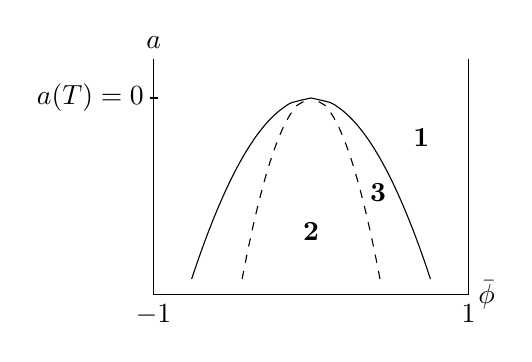
\begin{tikzpicture}
    \draw (-2, 3) node [above] {$a$} -- (-2, 0) node [below] {$-1$} -- (2, 0) node [below] {$1$} node [right] {$\bar \phi$} -- (2, 3);
    \node [left] at (-2, 2.5) {$a(T) = 0$};

    \draw [domain=2.5:0.2, samples=40] plot [smooth] ({sqrt (2.5 - \x)}, \x);
    \draw [domain=2.5:0.2, samples=40] plot [smooth] ({-sqrt (2.5 - \x)}, \x);

    \draw [dashed, domain=0.2:2.5] plot [smooth] ({sqrt ((2.5 - \x)/3)}, \x);
    \draw [dashed, domain=0.2:2.5] plot [smooth] ({-sqrt ((2.5 - \x)/3)}, \x);
    \draw (-2.05, 2.5) -- (-1.95, 2.5);

    \node at (1.4, 2) {$\mathbf{1}$};
    \node at (0.85, 1.3) {$\mathbf{3}$};
    \node at (0, 0.8) {$\mathbf{2}$};
  \end{tikzpicture}
\end{center}
Here $\bar{\phi}$ is the global composition, which is a control variable.

In the past, we discussed what the field looks like in each region when we are at equilibrium. At (1), the system is in a uniform phase that is globally stable. If we set up our system at (1), and then rapidly change the temperature so that we lie in (2) or (3), then we know that after the system settles, we will have a phase separated state. However, how this transition happens is not something mean field theory tells us. Heuristically, we expect

\begin{itemize}
  \item In (2), we have $|\bar{\phi}| < \phi_S$, and $f''(\phi) < 0$ implies local instability. The system rapidly becomes phase separated. This is \term{spinodal behaviour}.
  \item In (3), we have $\phi_S < |\bar{\phi}| < \phi_B$. A uniform phase is locally stable, but not globally. To reach the phase separated state, we need nucleation and growth to occur, and requires the contribution of noise.
\end{itemize}
We now study these in detail.
\subsubsection*{Regime 1}
We know that regime (1) is stable, and we shall see how it responds to perturbation about $\phi(r) = \bar{\phi}$. Put
\[
  \phi = \bar{\phi} + \tilde{\phi}(\mathbf{r}).
\]
We can then write
\[
  \mu = \frac{\delta F}{\delta \phi} = \frac{\partial f}{\partial \phi} - \kappa \nabla^2 \phi = f'(\bar{\phi}) + \tilde{\phi} f''(\bar{\phi}) - \kappa \nabla^2 \tilde{\phi}.
\]
Note that the first term is a constant. We then have
\begin{align*}
  \dot{\phi} &= - \nabla \cdot \mathbf{J}\\
  \mathbf{J} &= -M \nabla [f''\tilde{\phi} - \kappa \nabla^2 \tilde{\phi}] + \sqrt{2k_B T M} \boldsymbol\Lambda.
\end{align*}
We drop the tildes and take the Fourier transform to get
\[
  \dot{\phi}_{\mathbf{q}} = - M q^2 (f'' + \kappa q^2)\phi_{\mathbf{q}} + i\mathbf{q} \cdot \sqrt{2k_B TM} \boldsymbol\Lambda_{\mathbf{q}}.
\]
Compare this with an overdamped particle in a simple harmonic oscillator,
\[
  V = \frac{1}{2} \kappa x^2,
\]
where we have
\[
  \dot{x} = - \tilde{M} \kappa x + \sqrt{2k_B T \tilde{M}} \Lambda.
\]
Indeed, we can think of our system as an infinite family of decoupled harmonic oscillators, and solve each of them independently.

In the second example sheet, we compute
\[
  S(\mathbf{q}, t) \equiv \bra \phi_\mathbf{q}(0) \phi_{-\mathbf{q}} (t)\ket = S(q) e^{-r(q) t},
\]
This \term{$S(\mathbf{q}, t)$} is called the \term{dynamic structure factor}, which can be measured by light scattering. This doesn't say the fluctuations go away completely --- we expect there to be fluctuations all the time. What this says is that fluctuations at late times come completely from the random noise, and not the initial fluctuations.

%Here $s(q)$ is the equilibrium equal time static correlator, which is
%\[
%  \frac{k_B T}{f'' + \kappa q^2}.
%\]
\subsubsection*{Regime 2}
Consider the case where we are in the second regime. As before, we have the equation
\[
  \dot{\phi}_{\mathbf{q}} = - \underbrace{M q^2 (f'' + \kappa q^2)}_{r(q)}\phi_\mathbf{q} + i\mathbf{q} \cdot \sqrt{2k_B TM} \boldsymbol\Lambda_{\mathbf{q}},
\]
but crucially, now $f''(\bar{\phi}) < 0$, so it is possible to have $r(q) < 0$. The system is unstable.

If we ignore the noise by averaging the equation, then we get
\[
  \bra \dot{\phi}_\mathbf{q}\ket = - r(q) \bra \phi_q\ket.
\]
So if we have a noisy initial state $\phi_\mathbf{q}(0)$, then the perturbation grows as
\[
  \bra \phi_\mathbf{q}(t)\ket = \phi_\mathbf{q}(0) e^{-r(q)t}.
\]
When $r(q) < 0$, then this amplifies the initial noise. In this world, even if we start with a perfectly uniform $\phi$, noise terms will kick in and get amplified over time. Moreover, since we have an exponential growth, the earliest noise gets amplified the most, and at late times, the new perturbations due to the noise are negligible.

We can plot our $r(q)$ as follows:
\begin{center}
  \begin{tikzpicture}
    \draw [->] (0, 0) -- (4, 0) node [right] {$q$};
    \draw [->] (0, -1.3) -- (0, 3) node [above] {$r(q)$};
    \draw [domain=0:3.8, thick, mblue] plot [smooth] (\x, {\x^2 * (-2 + \x^2/5) / 5});

    \draw [dashed] (2.236, -1) -- (2.236, 0) node [above] {$q^*$};
  \end{tikzpicture}
\end{center}
The maximally unstable mode $q^*$ is given by the solution to $r'(q^*) = 0$, which we can easily check to be given by
\[
  q^* = \sqrt{\frac{-f''}{2\kappa}}.
\]
Now consider the equal time \term{non-equilibrium structure factor}\index{$S_\mathbf{q}(t)$}
\[
  S_\mathbf{q}(t) = \bra \phi_\mathbf{q}(t) \phi_{-\mathbf{q}}(t)\ket \sim S_\mathbf{q}(0) e^{-2r(q) t}.
\]
As time evolves, this gets more and more peaked around $q = q^*$:
\begin{center}
  \begin{tikzpicture}
    \draw [->] (0, 0) -- (4, 0) node [right] {$q$};
    \draw [->] (0, 0) -- (0, 3) node [above] {$S_\mathbf{q}(t)$};

    \draw[domain=0:4, mblue, semithick] plot [smooth] (\x, {0.1 + 0.02 * sin(500 * \x)});
    \draw[domain=0:4, mblue!25!mgreen, semithick] plot [smooth] (\x, {0.1 * e^(- \x^2 * (-2 + \x^2/5) / 5)});
    \draw[domain=0:4, mblue!50!mgreen, semithick] plot [smooth] (\x, {0.1 * e^(-2* \x^2 * (-2 + \x^2/5) / 5)});
    \draw[domain=0:4, mgreen!75!mgreen, semithick] plot [smooth] (\x, {0.1 * e^(-2.8* \x^2 * (-2 + \x^2/5) / 5)});
    \draw[domain=0:4, mgreen, semithick] plot [smooth] (\x, {0.1 * e^(-3.3* \x^2 * (-2 + \x^2/5) / 5)});
    \draw [dashed] (2.236, 3) -- (2.236, 0) node [below] {$q^*$};
  \end{tikzpicture}
\end{center}
So we see a growth of random structure with scale $L \sim \pi/q^*$. This process is called \term{spinodal decomposition}.
\begin{center}
  \begin{tikzpicture}
    \draw (0, 0) rectangle (3, 3);
    \draw [fill=mblue, fill opacity=0.3] plot [smooth] coordinates {(0.7, 0) (0.5, 0.9) (0.8, 1.5) (1, 2.5) (3, 2.3)} -- (3, 3) -- (0, 3) -- (0, 0);

    \draw [fill=mblue, fill opacity=0.3] (1.4, 0.7) circle [radius=0.3];

    \draw [fill=mblue, fill opacity=0.3] plot[smooth] coordinates {(3, 1.8) (1.8, 2) (1.7, 1.5) (3, 1.2)};

    \draw [fill=mblue, fill opacity=0.3] plot[smooth] coordinates {(3, 0.5) (2.3, 0.8) (2.2, 0.2) (2.6, 0)} -- (3, 0);

    \draw [-latex'] (1.7, 0.7) -- (2.21, 0.6) node [pos=0.5, above] {\small $L$};
    \draw [-latex'] (2.21, 0.6) -- (1.7, 0.7);
  \end{tikzpicture}
\end{center}
Note that this computation was done on the assumption that $\tilde{\phi}$ is small, where we ignored the quadratic terms. At intermediate $t$, as these phase separated states grow, the quartic terms are going to kick in. An informal use of variational theory says we should replace $f''$ by $\bar{f}''$, where
\[
  \bar{f}'' = f'' + \frac{3b}{(2\pi)^4} \int^{q_{max}} S_q(t) \;\d^d \mathbf{q}.
\]
This says $\bar{f}''$ is less negative as the fluctuations grow. Since
\[
  q^* = \sqrt{\frac{-\bar{f}''}{2k}},
\]
this moves to a smaller $q$. So $L(t) \sim \pi/q^*(t)$ starts increasing. This is called \term{domain growth}.

In the late stages, we have large regions of $\phi \approx \pm \phi_B$, so it is almost in equilibrium locally. We are well away from the exponential growth regime, and the driving force for domain growth is the reduction of interfacial area. We can estimate the free energy (per unit volume) as
\[
  \frac{F}{V} = \frac{\sigma A(t)}{V},
\]
where $A(t)$ is the area of the interface. So by dimensional analysis, this is $\sim \sigma/L(t)$. We have calculated the interfacial surface tension $\sigma$ before to be
\[
  \sigma = \left(\frac{-8\kappa a^3}{9b^2}\right)^{1/2},
\]
but it doesn't really matter what this is. The ultimate configuration with minimal surface area is when we have complete phase separation. The result is that
\[
  L(t) \sim \left(\frac{M_\sigma}{\phi_B} t\right)^{1/3}.
\]
We will not derive this yet, because this result is shared with the late time behaviour of the third regime, and we will discuss this at that point.

\subsubsection*{Regime 3}
Finally, consider the third regime. Suppose we have $\bar{\phi} = -\phi_B + \delta$, where $\delta$ is small. The system is locally stable, so $r(q) > 0$ for all $q$. On the other hand, it is globally unstable, so phase separation is preferred. To achieve phase separation, we must overcome a \term{nucleation barrier}, and we must rely on noise to do that.

To understand how the process will look like, formally, we can inspect the path probabilities
\[
  \P[\phi(\mathbf{r}, t)] = \mathcal{N} \exp \left(-\frac{\beta}{4M} \int |\mathbf{J} + M \nabla \mu|^2 \;\d \mathbf{r} \;\d t\right)
\]
given by the Langevin equation. We seek to find the most likely trajectory from the initial to the final state. In field theory, this is called the \term{instanton path}, and in statistical physics, this is called \term{large deviation theory}. Instead of doing this, we use our physical intuition to guide ourselves.

Heuristically, we expect that if we start with a uniform phase $\phi = -\phi_B + \delta$, then at some point, there will be some random small droplet with $\phi = +\phi_B$ of small radius $R$. This is already unlikely, but after this, we need $R$ to increase until we have full phase separation. The key question is --- how unlikely is this process?
\begin{center}
  \begin{tikzpicture}[scale=0.8]
    \draw (0, 0) rectangle (2, 2);
    \draw [->] (2.3, 1) -- (3.2, 1);
    \begin{scope}[shift={(3.5, 0)}]
      \draw (0, 0) rectangle (2, 2);
      \draw [fill=mblue, fill opacity=0.5] (1, 1) circle [radius=0.05];
      \draw [->] (2.3, 1) -- (3.2, 1);
    \end{scope}

    \begin{scope}[shift={(7, 0)}]
      \draw (0, 0) rectangle (2, 2);
      \draw [fill=mblue, fill opacity=0.5] (1, 1) circle [radius=0.1];
      \draw [->] (2.3, 1) -- (3.2, 1);
    \end{scope}

    \begin{scope}[shift={(10.5, 0)}]
      \draw (0, 0) rectangle (2, 2);
      \draw [fill=mblue, fill opacity=0.5] (1, 1) circle [radius=0.3];
    \end{scope}
  \end{tikzpicture}
\end{center}
The idea is to consider the cost of having a droplet of radius $R$. First there is the cost of having an interface, which is $4 \pi \sigma R^2$. However, the fact that we have $+\phi_B$ areas is energetically favorable, and this grows as the volume. So we get a cubic term $\sim -R^3$. If we add these two together, we get a barrier:
\begin{center}
  \begin{tikzpicture}
    \draw [->] (0, 0) -- (4, 0) node [right] {$R$};
    \draw [->] (0, -1.8) -- (0, 2.5) node [above] {$F(R)$};

    \draw [domain=0:3.7, mblue, semithick] plot [smooth] (\x, {3*(\x^2/3 -\x^3/10)});

    \draw [dashed] (2.222, 1.6461) -- (2.222, 0) node [below] {$R^*$};
    \draw [dashed] (2.222, 1.6461) -- (0, 1.6461) node [left] {$F^*$};
  \end{tikzpicture}
\end{center}
Once $R > R^*$, it is then energetically favorable for the radius to continue increasing, and then we can easily reach phase separation. To reach this, we must rely on noise to push us over this barrier, and this noise-induced rate is $\sim e^{-\beta F^*}$. To see what happens afterwards, we need to better understand how droplets work.

\subsubsection*{Droplet in equilibrium}
The mechanics of a droplet is slightly less straightforward than what one might hope, due to the presence of surface tension that tries to compress the droplet. The result is that the value of $\phi$ inside and outside the droplet is not exactly $\pm \phi_B$, but with a shift.

For simplicity, we shall first consider an \emph{equilibrium} system with a droplet. This is achieved by having a large box of fluid with $\bar{\phi}$ just slightly above $-\phi_B$. Then in the phase separated state, the $+\phi_B$ phase will lump together in a droplet (if we had $\bar{\phi} = 0$, then we would have a horizontal interface).
\begin{center}
  \begin{tikzpicture}
    \draw (0, 0) rectangle (3, 3);
    \draw [fill=mblue, fill opacity=0.5] (1.5, 1.5) circle [radius=0.6];
    \node at (1.5, 1.5) {$2$};
    \node at (2.4, 2.4) {$1$};
  \end{tikzpicture}
\end{center}
Within each region $1$ and $2$, the value of $\phi$ is constant, so the term that contributes to the free energy is
\[
  f (\phi) = \frac{a}{2} \phi^2 + \frac{b}{4} \phi^4.
\]
We would expect $1$ and $2$ to respectively be located at
\begin{center}
  \begin{tikzpicture}
    \draw [->] (-2.3, 0) -- (2.3, 0) node [right] {$\phi$};
    \draw [->] (0, -1.2) -- (0, 2.5) node [above] {$f$};
    \draw [domain=-2.15:2.15, mred, thick] plot [smooth] (\x, {-(\x)^2 + (\x)^4/3});

    \draw (-1.21, -0.65) -- (-1.21, -0.85) node [below] {$1$};
    \draw (1.24, -0.65) -- (1.24, -0.85) node [below] {$2$};
  \end{tikzpicture}
\end{center}
When we have a spherical interface, $1$ and $2$ are not exactly at $\pm \phi_B$. To see this, Consider the \term{bulk chemical potential}
\[
  \mu = \frac{\partial f}{\partial \phi},
\]
The thermodynamic pressure is then
\[
  \Pi = \mu \phi - f.
\]
This is the negative of the $y$-intercept of the tangent line at $\phi$.

If we have a flat interface, which we can think of as the limit $R \to \infty$, then we require
\[
  \mu_1^{bulk} = \mu_2^{bulk},\quad \Pi_1^{bulk} = \Pi_2^{bulk}.
\]
This means the points 1, 2 have a common tangent
\begin{center}
  \begin{tikzpicture}
    \draw [->] (-2.3, 0) -- (2.3, 0) node [right] {$\phi$};
    \draw [->] (0, -1.2) -- (0, 2.5) node [above] {$f$};
    \draw [domain=-2.15:2.15, mred, thick] plot [smooth] (\x, {-(\x)^2 + (\x)^4/3});

    \draw (-1.2247, -0.65) -- (-1.2247, -0.85) node [below] {$1$};
    \draw (1.2247, -0.65) -- (1.2247, -0.85) node [below] {$2$};

    \draw [dashed] (-2.3, -0.75) -- (2.3, -0.75);
  \end{tikzpicture}
\end{center}

If we have a droplet, then there is surface tension. Consider an imaginary interface between the upper and lower interface. Then the pressure difference tries to move the upper hemisphere up, and contributes a force of $(\Pi_2 - \Pi_1) \pi R^2$, while the interfacial tension pulls the boundary down by $2\pi R \sigma$. In general, in $d$ dimensions, we require
\[
  \Pi_2 = \Pi_1 + \frac{\sigma}{R}(d - 1)
\]
This is called the \term{Laplace pressure}.

In static equilibrium, we still require $\mu_1 = \mu_2$, since this is the same as saying $\mathbf{J} = \nabla \mu = 0$. So $f$ has the same slope at $\phi_1$ and $\phi_2$. However, the two tangent lines no longer have a common intercept, but they are separated by $\frac{\sigma}{R}(d - 1)$. So it looks like
\begin{center}
  \begin{tikzpicture}
    \draw [->] (-2.3, 0) -- (2.3, 0) node [right] {$\phi$};
    \draw [->] (0, -1.2) -- (0, 2.5) node [above] {$f$};
    \draw [domain=-2.15:2.15, mred, thick] plot [smooth] (\x, {-(\x)^2 + (\x)^4/3});

    \draw (-1.18, -0.646) -- (-1.18, -0.846) node [below] {$\phi_1$};
    \draw (1.27, -0.6458) -- (1.27, -0.8458) node [below] {$\phi_2$};

    \draw [dashed] (2, -0.6062) -- (-1, -1.1797);
    \draw [dashed] (-2, -0.88496) -- (1, -0.31);

    \draw [-latex] (-0.1, -0.988533) -- (-0.1, -0.501653) node [pos=0.4, left] {\scalebox{0.6}{$\Pi_2\!-\!\Pi_1$}\!};
    \draw [-latex] (-0.1, -0.501653) -- (-0.1, -0.988533);
  \end{tikzpicture}
\end{center}

To solve for this, we take the approximation that $\delta$ is small for $R$ decently large. Then we can write
\begin{align*}
  f_1 &= f(-\phi_B + \delta_1) \approx \frac{1}{2} f''(-\phi_B) \delta_1^2 + f(-\phi_B)\\
  f_2 &= f(+\phi_B + \delta_2) \approx \frac{1}{2} f''(+\phi_B) \delta_1^2 + f(+\phi_B).
\end{align*}
So $\mu_i = \alpha \delta_i$, where $\alpha = f''(\pm\phi_B)$. So we find that up to first order, $\delta_1 = \delta_2$.

To compute $\delta$, we compute
\[
  \Pi_1 = \mu_1\phi_1 - f_1 = -\alpha \delta \phi_B.
\]
Similarly, we have $\Pi_2 = +\alpha \delta \phi_B$. So
\[
  \Pi_1 - \Pi_2 = -2\alpha \phi_B \delta.
\]
Since this equals $-(d - 1)\frac{\sigma}{R}$, we have
\[
  \delta = \frac{d - 1}{2\alpha \phi_B} \cdot \frac{\sigma}{R}.
\]

\subsubsection*{Multiple droplet dynamics}
We now move on to understand multiple droplet dynamics. This is relevant because we expect that noise will produce multiple droplets around the fluid, which will then interact and combine to a single phase separated state.

The way droplets interact with each other is that once we have a droplet of large $\phi$, then the average $\phi$ outside of the droplet will decrease. So to begin understanding this scenario, we first see how a droplet reacts when the relative density of the outside bath is not what it expects.

So suppose we have a (3D) droplet of radius $R$ inside a bath with $\phi = - \phi_B + \varepsilon$, where $\varepsilon \not= \delta = \delta(R)$. This $\varepsilon$ is called the \term{supersaturation}. Note that to have a droplet of radius $R$, the value of $\phi$ inside and immediately outside the droplet must be $\pm \phi_B + \delta$. Outside of the droplet, the value of $\phi$ will slowly decay to $-\phi_B + \varepsilon$. Thus, outside of the droplet, we write
\[
  \phi(\mathbf{r}) = -\phi_B+ \tilde{\phi}(\mathbf{r}),
\]
where $\tilde{\phi}(\infty) = \varepsilon$ and $\tilde{\phi}(R^+) = \delta$.

In this situation, unless $\delta$ happens to be $\varepsilon$, we have a gradient of $\phi$, hence a gradient of chemical potential, hence a flux. Again in Model B, we have
\[
  \dot{\phi} = - \nabla \cdot \mathbf{J},\quad \mathbf{J} = -M \nabla \mu = -M \alpha \nabla \tilde{\phi}(\mathbf{r}),
\]
assuming a weak enough gradient. We assume this has a quasi-static behaviour, which is reasonable since molecules move quickly relative to how quickly the droplet changes in size. So to solve for $\tilde{\phi}(\mathbf{r})$ at any point in time, we set $\dot{\phi} = 0$. So $\nabla^2 \tilde{\phi} = 0$. We solve this with boundary conditions
\[
  \tilde{\phi}(\infty) = \varepsilon,\quad \tilde{\phi}(R^+) = \delta.
\]
So we have
\[
  \tilde{\phi} = \varepsilon + (\delta - \varepsilon) \frac{R}{r}.
\]
Now if we assume this is what $\tilde{\phi}(\mathbf{r})$ looks like, then the current just outside the droplet gives
\[
  \mathbf{J}(R^+) = -M \nabla \mu = - \alpha M \left.\frac{\partial \tilde{\phi}}{\partial r}\right|_{R^+} = \alpha M(\delta - \varepsilon) \left.\frac{B}{r^2}\right|_{r = R^+} = \frac{\alpha M(\delta - \varepsilon)}{R}.
\]
Thus, when $\delta$ and $\varepsilon$ are not the same, there is a flow of fluid in or out of the droplet. The discontinuity in $\phi$ across the boundary is $\Delta \phi = 2 \phi_B$. So mass conservation implies
\[
  2 \phi_B \dot{R} = - J = - \frac{\alpha M (\delta - \varepsilon)}{R}.
\]
Thus, we conclude that
\[
  \dot{R} = \frac{1}{2 \phi_B} \left(\frac{\alpha M}{R} (\varepsilon - \delta(R))\right).
\]
We can plug in our previous expression for $\delta$. Fixing $\varepsilon$, we can plot $\dot{R}$ as follows:
\begin{center}
  \begin{tikzpicture}
    \draw (0, 0) -- (3, 0) node [right] {$R$};
    \draw (0, -1.5) -- (0, 1.5) node [above] {$\dot{R}$};
    \draw [domain=0.56:3, thick, mblue] plot [smooth] (\x, {2/\x * ( 1.4 - 1/\x)});

    \node at (0.714, 0) [anchor = north west] {$R^*$};
    \node [circ, mblue] at (0.714, 0) {};
  \end{tikzpicture}
\end{center}
where
\[
  R^* = \frac{\sigma}{\alpha \varepsilon \phi_B}.
\]
So if we have a bath containing many droplets, then the big droplets grow and the small droplets shrink. Indeed, the interfacial tension penalizes small droplets more heavily than large droplets.

To understand exactly how these grow, we make a scaling ansatz that there is only one length scale, namely the mean droplet size $\bar{R}$. Then we have
\[
  \dot{\bar{R}} \approx \frac{1}{2\phi_B} \frac{\alpha M}{\bar{R}} (\varepsilon - \delta(\bar{R})).
\]
We know that the value of $\varepsilon$ is also determined by $\bar{R}$, so we know $\varepsilon - \delta (\bar{R})$ is of order $\delta (\bar{R})$. Hence
\[
  \dot{\bar{R}} \sim \frac{M\sigma}{\phi_B^2 \bar{R}^2}
\]
So
\[
  \bar{R}^3 \sim \frac{M\sigma t}{\phi_B^2}.
\]
So the typical droplet size is $\sim t^{1/3}$. Likewise, $R^* \sim t^{1/3}$, and so $\varepsilon \sim t^{-1/3}$.

So if we have a sea of droplets, they go into this competitive process, and we get fewer and fewer droplets of larger and larger size. This is called \term{Ostwald ripening}, and is a diffusive coarsening mechanism.

We have the same scaling for non-droplet geometries, e.g.\ spinodal decomposition at late times. In this case, our domains flatten and enlarge, and we have
\[
  L(t) \sim \left(\frac{M\sigma}{\phi_B^2} t\right)^{1/3}.
\]

In practice, we often want to stop this from happening. One way to do so is to add trapped species insoluble in the continuous phase, e.g.\ polymers or salt. If there are $N$ particles inside the droplet exerting ideal gas pressure, then we have
\[
  \Pi_2 - \Pi_1 = \frac{2\sigma}{R} + \frac{Nk_B T}{4/3 \pi R^3},
\]
We again have $\mu_1 = \mu_2$. This ends up giving a new boundary condition at $R^+$,
\[
  \tilde{\phi}(R^+) = \frac{\sigma}{\alpha R \phi_B} - \frac{3N k_B T}{8 \alpha \phi_B \pi R^3} = \frac{1}{2 \alpha \phi_B} (\Pi_{\mathrm{Lap}} - \Pi_{\mathrm{sol}})
\]
The first term is the Laplace pressure just as before, while the second term is the extra term from the trapped species.

If we put this back into the system of equations before, then we have a new equation of motion
\[
  \dot{R} = \frac{1}{2 \phi_B} \left( \frac{\alpha M}{R} \left(\varepsilon - \frac{\sigma}{\alpha \phi_B R} + \frac{3 N k_B T}{8 \alpha \phi_B \pi R^3}\right)\right).
\]
\begin{center}
  \begin{tikzpicture}
    \draw [->] (0, 0) -- (4, 0) node [right] {$R$};
    \draw [->] (0, -1) -- (0, 2) node [above] {$\dot{R}$};
    \draw [mblue, semithick, domain=0.65:1.5] plot (\x, {1/\x (1 - 3/\x + 1.5/\x^3)});
    \draw [mblue, semithick, domain=1.5:4] plot (\x, {1/\x (1 - 3/\x + 1.5/\x^3)});
    \node [circ] at (0.832, 0) {};
    \node [anchor = north east] at (0.832, 0) {$R_s$};
  \end{tikzpicture}
\end{center}
We now see that there is a stable fixed point $R_s$, and further shrinkage is prevented by the presence of the trapped species that will be further compressed by shrinking. Thus, if we manage to produce a system with all droplets of size $< R^*$, then we end up with a lot of small but finite size droplets $R_s$.

\section{Model H}
Model B was purely diffusive, and the only way $\phi$ can change is by diffusion. Often, in real life, fluid can flow as well. If the fluid has a velocity $\mathbf{v}$, then our equation is now
\[
  \dot{\phi} + \mathbf{v} \cdot \nabla \phi = - \nabla \cdot \mathbf{J}.
\]
The $\mathbf{v} \cdot \nabla \phi$ is called the \term{advection term}. Our current $\mathbf{J}$ is the same as before, with
\[
  \mathbf{J} = -M \frac{\delta F}{\delta \phi} + \sqrt{2k_B T M} \boldsymbol\Lambda.
\]
We also need an evolution equation for $\mathbf{v}$, which will be the Navier--Stokes equation with some noise term. We assume flow is incompressible, so $\nabla \cdot \mathbf{v} = 0$. We then have the Cauchy equation with stress tensor $\Sigma^{\mathrm{TOT}}$, given by
\[
  \rho(\dot{\mathbf{v}} + \mathbf{v} \cdot \nabla \mathbf{v}) = \nabla \cdot \Sigma^{\mathrm{TOT}} + \text{body forces}.
\]
We will assume there is no body force. This is essentially the momentum conservation equation, where $- \Sigma^{\mathrm{TOT}}$ is the momentum flux tensor.

Of course, this description is useless if we don't know what $\Sigma^{\mathrm{TOT}}$ looks like. It is a sum of four contributions:
\[
  \Sigma^{\mathrm{TOT}} = \Sigma^p + \Sigma^\eta + \Sigma^\phi + \Sigma^N.
\]
\begin{itemize}
  \item The $\Sigma^p$ term is the \term{pressure} term, given by
    \[
      \Sigma_{ij}^p = - P \delta_{ij}.
    \]
    We should think of this $P$ as a Lagrange multiplier for incompressibility.
  \item The $\Sigma^{\eta}$ term is the \term{viscous stress}, which we can write as
    \[
      \Sigma_{ij}^\eta = \eta (\nabla_i v_j + \nabla_j v_i)
    \]
    For simplicity, we assume we have a constant viscosity $\eta$. In general, it could be a function of the composition.
  \item The $\Sigma^{\phi}$ term is the \term{$\phi$-stress}, given by
    \[
      \Sigma^\phi = - \Pi \delta_{ij} - \kappa (\nabla_i \phi) (\nabla_j \phi),\quad \Pi = \phi \mu - F.
    \]
    This is engineered so that
    \[
      \nabla \cdot \Sigma^\phi = - \phi \nabla \mu.
    \]
    This says a non-constant chemical potential causes things to move to even that out.
  \item The final term is a \term{noise stress} with
    \[
      \bra \Sigma_{ij}^N (\mathbf{r}, t) \Sigma_{k\ell}^N (\mathbf{r}', t')\ket = 2k_B T \eta \left(\delta_{ik} \delta_{j\ell} + \delta_{i\ell} \delta_{jk} - \frac{2}{3} \delta_{ij} \delta_{k\ell}\right) \delta(\mathbf{r} - \mathbf{r}') \delta(t - t').
    \]
    The last term $\delta_{ij} \delta_{k\ell}$ is there to ensure the noise does not cause any compression. This is a white noise term whose variance is determined by the fluctuation dissipation theorem.
\end{itemize}
We can then compute
\begin{align*}
  \nabla \cdot \Sigma^{\mathrm{TOT}} &= \nabla \cdot \Sigma^P + \nabla \cdot \Sigma^\eta + \nabla \cdot \Sigma^\phi + \nabla \cdot \Sigma^N\\
  &= - \nabla P + \eta \nabla^2 \mathbf{v} + - \phi \nabla \mu + \nabla \cdot \Sigma^N
\end{align*}
Hence Model H has equations
\begin{align*}
  \dot{\phi} + \mathbf{v} \cdot \nabla \phi &=- \nabla \cdot \mathbf{J}\\
  \mathbf{J} &= -M \nabla \mu + \sqrt{2k_B T M} \boldsymbol\Lambda\\
  \nabla \cdot \mathbf{v} &= 0\\
  \rho (\dot{\mathbf{v}} + \mathbf{v} \cdot \nabla \mathbf{v}) &= \eta \nabla^2 \mathbf{v} - \nabla P - \phi \nabla \mu + \nabla \cdot \Sigma^N.
\end{align*}
Compared to Model B, we have the following new features:
\begin{enumerate}
  \item $-\phi\nabla \mu$ drives deterministic fluid flow.
  \item $\Sigma^N$ drives a \emph{random} flow.
  \item Fluid flow advects $\phi$.
\end{enumerate}
How does this affect the coarsening dynamics? We will see that (i) and (iii) gives us enhanced coarsening of bicontinuous states. However, this does not have any effect on isolated/disconnected droplet states, since in a spherically symmetric setting, $\phi \nabla \mu$ and $\nabla P$ will be radial, and so $\nabla \cdot \mathbf{v} = 0$ implies $\mathbf{v} = 0$. In other words, for $\phi \nabla \mu$ to drive a flow, we must have some symmetry breaking.

Of course, this symmetry breaking is provided by the noise term in (ii). The result is that the droplets will undergo Brownian motion with $\bra r^2\ket \sim Dt$, where
\[
  D = \frac{k_B T}{4\pi \eta R}
\]
is the diffusion constant.

If we think about the Ostwald process, even if we manage to stop the small droplets from shrinking, they may collide and combine to form larger droplets. This forms a new channel for instability, and separate measures are needed to prevent this. For example, we can put charged surfactants that prevent collisions.

We can roughly estimate the time scale of this process. We again assume there is one length scale $\bar{R}(t)$, which determines the size and separation of droplets. We can then calculate the collision time
\[
  \Delta t \simeq \frac{\bar{R}^2}{D(\bar{R})} \sim \bar{R}^3 \frac{\eta}{k_B T}.
\]
Each collision doubles the volume, and so $\bar{R} \to 2^{1/3} \bar{R}$. Taking the logarithm, we have
\[
  \Delta \log \bar{R} \sim \frac{\log 2}{3}\text{ in time }\Delta t.
\]
So we crudely have
\[
  \frac{\Delta \log \bar{R}}{\Delta t} \sim \frac{\log 2}{3} \frac{k_B T}{\eta \bar{R}^3}.
\]
If we read this as a differential equation, then we get
\[
  \frac{\d \log \bar{R}}{\d t} = \frac{1}{\bar{R}} \dot{\bar{R}} \sim \frac{k_B T}{\eta \bar{R}^3}.
\]
So we find that
\[
  \bar{R}^2 \dot{\bar{R}} \sim \frac{k_B T}{\eta}.
\]
So
\[
  \bar{R}(t) \sim \left(\frac{k_B T}{\eta} t\right)^{1/3}.
\]
This is \term{diffusion limited coalescence}.

Recall that in the Ostwald process, droplets grew by diffusion of molecules, and we had the same power of $t$. However, the coefficient was different, with
\[
  \bar{R} \sim \left(\frac{M \sigma}{\phi_B} t\right)^{1/3}.
\]
It makes sense that they have the same scaling law, because ultimately, we are still doing diffusion on different scales.

\subsubsection*{Bicontinuous states}
We now see what the fluid flow does to bicontinuous states.
\begin{center}
  \begin{tikzpicture}
    \draw (0, 0) rectangle (3, 3);
    \draw [fill=mblue, fill opacity=0.3] plot [smooth] coordinates {(0.7, 0) (0.5, 0.9) (0.8, 1.5) (1, 2.5) (3, 2.3)} -- (3, 3) -- (0, 3) -- (0, 0);

    \draw [fill=mblue, fill opacity=0.3] (1.4, 0.7) circle [radius=0.3];

    \draw [fill=mblue, fill opacity=0.3] plot[smooth] coordinates {(3, 1.8) (1.8, 2) (1.7, 1.5) (3, 1.2)};

    \draw [fill=mblue, fill opacity=0.3] plot[smooth] coordinates {(3, 0.5) (2.3, 0.8) (2.2, 0.2) (2.6, 0)} -- (3, 0);

    \draw [-latex'] (1.7, 0.7) -- (2.21, 0.6) node [pos=0.5, above] {\small $L$};
    \draw [-latex'] (2.21, 0.6) -- (1.7, 0.7);
  \end{tikzpicture}
\end{center}

Again assume we have a single length scale $L(t)$, given by the domain size. Again we assume we have a single length scale. As time goes on, we expect $L(t)$ to increase with time.

A significant factor in the evolution of the bicontinuous phase is the Laplace pressure, which is ultimately due to the curvature $K$. Since there is only one length scale, we must have
\[
  \dot{K} \sim v.
\]
The Laplace pressure then scales as $\sim \frac{\sigma}{L}$.

The noise terms $\Sigma^N$ matter at early times only. At late times, the domains grow deterministically from random initial conditions. The key question is how $L(t)$ scales with time. The equation of motion of the flow is
\[
  \rho(\dot{\mathbf{v}} + \mathbf{v} \cdot \nabla \mathbf{v}) = \eta \nabla^2 \mathbf{v} - \nabla P - \phi \nabla \mu,
\]
We make single length scale approximations as before, so that $v \sim \dot{L}$ and $\nabla \sim L^{-1}$. Then we have an equation of the form.
\[
  \rho \ddot{L} + \rho \frac{\dot{L}^2}{L} \sim \eta \frac{\dot{K}}{L^2} + \text{Lagrange multiplier} + \frac{\sigma}{L^2}\tag{$*$} % align as above.
\]
where we recall that at curved interfaces, $\mu \sim \pm \frac{\sigma}{R}$. Here we have a single variable $L(t)$, and three dimensionful parameters $\rho, \eta, \sigma$.
%Note that $\sigma$ depends on the coefficients $a, b, \kappa$ in $F$, but these $a, b, \kappa$ do not enter separately. They only do so via the combination $\sigma = \left(-\frac{8 \kappa a^3}{9b^2}\right)^{1/2}$, and not via the interfacial thickness $\xi = \left(-\frac{2\kappa}{a}\right)^{1/2}$. This is not surprising, since the interfacial thickness is very small relative to the length scale $L(t)$.
We can do some dimensional analysis. In $d$ dimensions, we have
\[
  \rho = ML^{-d},\quad \eta = M L^{2 - d} T^{-1},\quad \sigma = ML^{3 - d} T^{-2}.
\]
We want to come up with combinations of these for length to depend on time, and we find that in three dimensions, we have
\[
  L_0 = \frac{\eta^2}{\rho \sigma},\quad t_0 = \frac{\eta^3}{\rho \sigma^2}.
\]
One can check that these are the only combinations with units $L, T$. So we must have
\[
  \frac{L(t)}{L_0} = f \left(\frac{t}{t_0}\right).
\]
We now substitute this into the equation $(*)$. We then get a non-dimensionalized equation for $(*)$
\[
  \alpha f'' + \beta f'^2/f = \gamma \frac{f'}{f^2} + \frac{\delta}{f^2},
\]
with $\alpha, \beta, \gamma, \delta = O(1)$ dimensionless numbers.

If we think about this, we see there are two regimes,
\begin{enumerate}
  \item The LHS (inertia) is negligible at small $t/t_0$ (or small $f$). Then we get
    \[
      \frac{\gamma f'}{f^2} + \frac{\delta}{f^2} = 0,
    \]
    so $f'$ is a constant, and so $L$ grows linearly with $t$. Putting all the appropriate constants in, we get
    \[
      L \propto \frac{\sigma}{\eta} t.
    \]
    This is called the \term{viscous hydrodynamic regime}, \term{VH}.

  \item For large $f$, we assume we have a power law $f(x) \sim x^y$, where $y > 0$ (or else $f$ would not be large). Then
    \[
      \bar{\alpha} x^{y - 2} + \bar{\beta} x^{y - 2} = \bar{\gamma} x^{-y - 1} + \delta x^{-2y}.
    \]
    It turns out at large $f$, the $x^{-y - 1}$ term is negligible, scaling wise. So we have $y - 2 = -2y$, or equivalently, $y = \frac{2}{3}$. So
    \[
      \frac{L}{L_0} \sim \left(\frac{t}{t_0}\right)^{2/3}.
    \]
    Putting back our factors, we have
    \[
      L \sim \left(\frac{\sigma}{\rho}\right)^{1/3} t^{2/3}.
    \]
    This is called the \term{inertial hydrodynamic regime}, \term{IH}. In this regime, interfacial energy is converted into kinetic energy, and then only ``later'' dissipated by $\eta$.
\end{enumerate}
Essentially, in the first regime, the system is overdamped. This happens until the right-hand side becomes big and takes over, until the viscous term finally takes over. In practice, it is difficult to reach the last regime in a lab, since the time it takes is often $\sim 10^4$.

%The outcome for $d = 3$ is
%\begin{center}
%  \begin{tikzpicture}
%    \draw [->] (0, 0) -- (4, 0) node [right] {$\log (t/t_0)$};
%    \draw [->] (0, 0) -- (0, 3) node [above] {$\log (L/K_0)$};
%
%
%  \end{tikzpicture}
%\end{center}
%The crossover is at $\frac{t^*}{t_0} \sim O(1)$.

\subsubsection*{Droplet vs bicontinuous}
In general, when do we expect a bicontinuous phase and when do we expect a droplet phase?
%Recall we had the phase diagram
%\begin{center}
%  \begin{tikzpicture}
%    \draw (-2, 3) node [above] {$a$} -- (-2, 0) node [below] {$-1$} -- (2, 0) node [below] {$1$} node [right] {$\bar \phi$} -- (2, 3);
%
%    \draw [domain=2.5:0.2, samples=40] plot [smooth] ({sqrt (2.5 - \x)}, \x);
%    \draw [domain=2.5:0.2, samples=40] plot [smooth] ({-sqrt (2.5 - \x)}, \x);
%
%    \draw [dashed, domain=0.2:2.5] plot [smooth] ({sqrt ((2.5 - \x)/3)}, \x);
%    \draw [dashed, domain=0.2:2.5] plot [smooth] ({-sqrt ((2.5 - \x)/3)}, \x);
%    \draw (-2.05, 2.5) -- (-1.95, 2.5);
%  \end{tikzpicture}
%\end{center}
%Suppose we start with a global composition $\bar{\phi}$ at large $a$, and quench the system so that we are now in the spinodal region. The conservation laws require
%\begin{align*}
%  - \phi_B V_a + \phi_B V_2 &= \bar\phi V\\
%  V_1 + V_2 &= V
%\end{align*}
%
%We can then define the \term{phase volume}
%\[
%  \psi = \frac{V_2}{ V},
%\]
%which we can find by
%\[
%  \psi = \frac{1}{2} \left(1 + \frac{\bar{\phi}}{\phi_B}\right).
%\]
%When this is sufficiently far away from $\frac{1}{2}$, we have droplets, and when this is close to $\frac{1}{2}$, we have a bicontinuous medium.

\begin{itemize}
  \item In three dimensions, the rule of thumb is that if $\psi \sim 0.4 \text{ to }0.6$, then we always get a bicontinuous medium. If $\psi < 0.3$ or $>0.7$, then we get droplets always. In between these two regions, we initially have bicontinuous medium, which essentially de-percolates into droplets.
  \item In two dimensions, things are different. In the fully symmetric case, with a constant $\eta$ throughout, and $F$ is strictly symmetric ($F(\phi) = F(-\phi)$), the \emph{only} case where we have bicontinuous phase is on the $\psi = \frac{1}{2}$ line.
\end{itemize}

%Note that for droplets, we have $\psi \sim \frac{R^3}{L^3}$, where $R$ is the droplet size and $L$ is the droplet separation. Since we have a fixed $\psi$, it follows that $R \sim L$.


%We can get a ``mixed'' Ostwald and fluid flow, and is complicated and difficult to understand.

\section{Liquid crystals hydrodynamics}
\subsection{Liquid crystal models}
We finally turn to the case of liquid crystals. In this case, our order parameter no longer takes a scalar value, and interesting topological phenomena can happen. We first write down the theory in detail, and then discuss coarsening behaviour of liquid crystals. We will describe the coarsening purely via geometric means, and the details of the model are not exactly that important.

Recall that there are two types of liquid crystals:
\begin{enumerate}
  \item Polar liquid crystals, where the molecules have ``direction'', and the order parameter is $\mathbf{p}$, a vector, which is orientational but not positional.
  \item Nematic liquid crystals, where the molecules are like a cylinder, and there is an order parameter $\boldsymbol\Theta$.
\end{enumerate}

We will do the polar case only, and just quote the answers for the nematic case.

As before, we have to start with a free energy
\[
  F = \int \left\{\frac{a}{2} |\mathbf{p}|^2 + \frac{b}{4} |\mathbf{p}|^4 + \frac{\kappa}{2} (\nabla_i \mathbf{p}_j)(\nabla_i p_j)\right\}\;\d \mathbf{r} \equiv \int \F \;\d \mathbf{r}.
\]
The first two terms are needed for the isotropic-polar transition to occur. Note that
\begin{enumerate}
  \item $F[\mathbf{p}] = F[-\mathbf{p}]$, so we have no cubic term.
  \item A linear term would correspond to the presence of an external field, e.g.\ magnetic field.
  \item The $\kappa$ term penalizes splay, twist and bend, and this term penalizes them roughly equally. This is called the \term{one elastic constant approximation}. If we want to be more general, we need something like
    \[
      \frac{\kappa_1}{2} |\nabla \cdot \mathbf{p}|^2 + \frac{\kappa_2}{2} |\hat{\mathbf{p}} \cdot \nabla \wedge \mathbf{p}|^2 + \frac{\kappa_3}{2} |\hat{\mathbf{p}} \wedge \mathbf{p}|^{2}.
    \]
\end{enumerate}
Here $\mathbf{p}$ is not conserved, so $\dot{\mathbf{p}}$ is not of the form $-\nabla \cdot \mathbf{J}$. Instead, (without flow) we have
\[
  \dot{\mathbf{p}} = - \Gamma \mathbf{h},\quad \mathbf{h} = \frac{\delta F}{\delta p(\mathbf{r})},
\]
where $\mathbf{h}(\mathbf{r})$ is called the \term{molecular field}, and $\Gamma$ is a constant, called the \term{angular mobility}.

We now want to generalize this to the case when there is a field flow. We can just write this as
\[
  \frac{\D p}{\D t} = - \Gamma \mathbf{h},
\]
where $\D$ is some sort of comoving derivative. For the scalar field, we had
\[
  \frac{\D \phi}{\D t} = \dot{\phi} + \mathbf{v} \cdot \nabla \phi.
\]
Note that the advective term is trilinear, being first order in $\mathbf{v}$, $\nabla$ and $\phi$. For $\mathbf{p}$, there is certainly something like this going on. If we have a translation, then $\mathbf{p}$ gets incremented by
\[
  \Delta \mathbf{p} = \mathbf{v} \cdot \nabla \mathbf{p}\;\Delta t,
\]
as for a scalar.

There is at least one more thing we should think about, namely if $\mathbf{v}$ is rotational, then we would expect this to rotate $\mathbf{p}$ as well. We have the corotational term
\[
  \Delta \mathbf{p} = \boldsymbol\omega \wedge \mathbf{p}\;\Delta t,
\]
where $\boldsymbol\omega$ is the angular velocity of the fluid, given by
\[
  \omega_i = \frac{1}{2} \varepsilon_{ijk} \Omega_{jk},\quad \Omega_{jk} = \frac{1}{2} (\nabla_i v_j - \nabla_j v_i).
\]
This part must be present. Indeed, if we rotate the whole system as a rigid body, with $\mathbf{v}(\mathbf{r}) = \boldsymbol\omega \times \mathbf{r}$, then we must have $\dot{\mathbf{p}} = \boldsymbol\omega \wedge \mathbf{p}$.

It turns out in general, there is one more contribution to the advection, given by
\[
  \Delta \mathbf{p} = - \xi \D \cdot \mathbf{p} \Delta t
\]
with $\D_{ij} = \frac{1}{2} (\nabla_i v_j + \nabla_j v_i)$ and $\xi$ a parameter. This is the irrotational part of the derivative. The reason is that in a general flow, $\mathbf{p}$ needn't simply rotate with $\boldsymbol\omega$. Instead, it typically aligns along streamlines. In total, we have
\[
  \frac{\D \mathbf{p}}{\D t} = (\partial_t + \mathbf{v} \cdot \nabla) \mathbf{p} + \Omega \cdot \mathbf{p} - \xi \D \cdot \mathbf{p}.
\]
The parameter $\xi$ is a molecular parameter, which depends on the liquid crystal. The $\xi = 1$ case is called \term{no slip}, and the $\xi = 0$ case is called \term{full slip}.

With this understanding, we can write the hydrodynamic equation as
\[
  \frac{\D \mathbf{p}}{\D t} = - \Gamma \mathbf{h},\quad \mathbf{h} = \frac{\delta F}{\delta \mathbf{p}}.
\]
We next need an equation of motion for $\mathbf{v}$. We can simply
\[
  \rho(\partial_t +\mathbf{v} \cdot \nabla) \mathbf{v} = \eta \nabla^2 \mathbf{v} - \nabla P + \nabla \cdot \Sigma^p,
\]
where $\Sigma^p$ is a stress tensor coming from the order parameter.

To figure out what $\Sigma^p$ should be, we can consider what happens when we have an ``advective'' elastic distortion. In this case, we have $\frac{\D \mathbf{p}}{\D t} = 0$, so we have
\[
  \dot{\mathbf{p}} = - \mathbf{v} \cdot \nabla \mathbf{p} - \Omega \cdot \mathbf{p} + \xi \D \cdot \mathbf{p},
\]
The free energy change is then
\[
  \delta F = \int \frac{\delta F}{\delta \mathbf{p}} \cdot \dot{\mathbf{p}}\; \Delta t \;\d \mathbf{r} = \Delta t \int \mathbf{h} \cdot \mathbf{p} \;\d \mathbf{r},
\]
On the other hand, the free energy change must also be given by
\[
  \delta F = \int \Sigma_{ij}^{\mathbf{p}} \nabla_i u_j(\mathbf{r}) \;\d \mathbf{r},
\]
the product of the stress and strain tensors. By matching these two expressions, we see that we can write
\[
  \Sigma_{ij}^p = \Sigma_{ij}^{(1)} + \Sigma_{ij}^{(2)} + \Sigma_{ij}^{(3)},
\]
where
\[
  \nabla_i \Sigma_{ij}^{(1)} = - p_k \nabla_j h_k,\quad
  \Sigma_{ij}^{(2)} = \frac{1}{2} (p_i h_j - p_j h_i),\quad
  \Sigma_{ij}^{(2)} = \frac{\xi}{2} (p_i h_j + p_j h_i).
\]

Analogous results for a nematic liquid crystal holds, whose derivation is a significant pain. We have
\[
  \frac{\D Q}{\D t} = - \Gamma H,\quad H_{ij} = \frac{\delta F}{\delta Q_{ij}} - \left( \Tr\frac{\delta F}{\delta Q}\right) \frac{\delta_{ij}}{d}.
\]
The second term in $H$ is required to ensure $Q$ remains traceless.

The total derivative is given by
\[
  \frac{\D Q}{\D t} = (\partial_t + \mathbf{v} \cdot \nabla) Q + (\Omega \cdot Q - Q \cdot \omega) + \xi (\D \cdot Q + Q \cdot D) - 2\xi \left(Q + \frac{\mathbf{1}}{d}\right) \Tr(Q \cdot \nabla \mathbf{v}).
\]
The terms are the usual advection term, rotation, alignment/slip and tracelessness terms respectively. The Navier--Stokes equation involves a stress term
\[
  \Sigma^Q = \Sigma^{Q, 1} + \Sigma^{Q, 2},
\]
where
\begin{align*}
  \nabla_k \Sigma^{Q, 1}_{k, \ell} &= - Q_{ij} \nabla_\ell H_{ij}\\
  \Sigma^{Q, 2} &= Q \cdot H - H \cdot Q - \xi \left(\frac{2}{3} H + 2 \widehat{QH} - 2 Q \tr (Q H)\right),
\end{align*}
with the hat denoting the traceless symmetric part. The rest of the Navier--Stokes equations is the same.

\subsection{Coarsening dynamics for nematics}
We will discuss the coarsening dynamics for nematic liquid crystals, and indicate how polar liquid crystals are different when appropriate. As before, we begin with a completely disordered phase with $Q = 0$, and then quench the system by dropping the temperature quickly. The liquid crystals then want to arrange themselves. Afterwards, we local have
\[
  Q =
  \begin{pmatrix}
    \lambda & 0 & 0\\
    0 & - \lambda/2 & 0\\
    0 & 0 & -\lambda/2
  \end{pmatrix}
\]
with free energy $f(\lambda)$. If the quench is deep enough, we have spinodal-like instability, and we quickly get locally ordered. Coordinate-independently, we can write
\[
  Q = \hat{\lambda} \left(n_i n_j - \frac{1}{3} \delta_{ij}\right).
\]
Since all this ordering is done locally, the principal axis $\mathbf{n}$ can vary over space. There is then a slower process that sorts out global ordering, driven by the elastic part of the free energy.

%we previously saw that there is still an energy barrier to overcome, and so we have to deal with nucleation.
%
%For a deep quench, we no longer have an energy barrier, and we have spinodal-like local instability. We have
%\[
%  \frac{\D Q}{\D t} = - \Gamma H,\quad H = \frac{\partial f}{\partial Q} - \kappa \nabla^2 Q.
%\]
%Going into Fourier space, the fastest growth occur at $q \to 0$, because of the second term which only slows us down at large $q$. This has a growth rate $r(0)$. So on a time scale of $r(0)^{-1}$, we know that $Q \to \diag(\lambda, -\lambda/2, -\lambda/2)$ almost everywhere. In other words,
%\[
%  Q = \hat{\lambda} \left(n_i n_j - \frac{1}{3} \delta_{ij}\right)
%\]
%However, in general, we expect the principal axes to depend on the point, since these orderings happen at different points independently. So we have $\mathbf{n} = \mathbf{n}(\mathbf{r})$. So we have a quick process that sorts out the local ordering, then there is a slow process that sorts out the global ordering. This is driven by the elastic part of the free energy. Recall that
%\[
%  \F = a \Tr(Q^2) + b (\Tr Q^2)^2 + b (\Tr Q^4) + c (\Tr Q^2) + \frac{\kappa}{2} (\nabla \cdot Q)^2,
%\]
%and the elastic term is the last one. So
%\[
%  \frac{\D Q}{\D t} = - \Gamma \frac{\delta F_{el}}{\delta Q} \sim - \nabla \nabla(\text{something}).
%\]
% like conserved quantity % goldstone's theorem, spontaneous symmetry breaking


Compare this with Model B/H: at early times, we have $\phi: \pm \phi_B$, but we get domain walls between the $\pm \phi_B$ phases.
\begin{center}
  \begin{tikzpicture}
    \draw [->] (-3, 0) -- (3, 0) node [right] {$x$};
    \draw [->] (0, -2) -- (0, 2) node [above] {$\phi$};

    \draw [mblue, thick, domain=-3:3] plot [smooth] (\x, {tanh(1.5*(\x + 1))});

    \draw [dashed] (-3, 1) -- (3, 1);
    \draw [dashed] (-3, -1) -- (3, -1);

  \end{tikzpicture}
\end{center}
The late time dynamics is governed by the slow coarsening of these domain walls. The key property of this is that it has reduced dimensionality, i.e.\ the domain wall is $2$ dimensional while space is $3$ dimensional, and it connects two different grounds states (i.e.\ minima of $F$).

The domain wall can be moved around, but there is no local change that allows us to remove it. They can only be removed by ``collision'' of domain walls.

Analogous structures are present for nematic liquid crystals. The discussion will largely involve us drawing pictures. For now, we will not do this completely rigorously, and simply rely on our intuitive understanding of when defects can or cannot arise. We later formalize these notions in terms of homotopy groups.

We first do this in two dimensions, where defects have dimension $< 2$. There can be no line defects like a domain wall. The reason is that if we try to construct a domain wall
\begin{center}
  \begin{tikzpicture}
    \draw (-2, -2) rectangle (2, 2);

     \foreach \y in {-1.5,-1,-0.5,0,0.5,1,1.5} {
       \foreach \x in {-1.25, -0.75, -0.25} {
         \draw [mblue, semithick] (\x - 0.1, \y - 0.1) -- (\x + 0.1, \y + 0.1);
         \draw [mblue, semithick] (-\x + 0.1, \y - 0.1) -- (-\x - 0.1, \y + 0.1);
       }
     }
  \end{tikzpicture}
\end{center}
then this can relax locally to become
\begin{center}
  \begin{tikzpicture}
    \draw (-2, -2) rectangle (2, 2);

     \foreach \y in {-1.5,-1,-0.5,0,0.5,1,1.5} {
       \foreach \x in {-1.25, -0.75, -0.25} {
         \draw [mblue, semithick] (\x - 0.1, \y + \x * 0.1 / 1.25) -- (\x + 0.1, \y - 0.1 * \x / 1.25);
         \draw [mblue, semithick] (-\x - 0.1, \y - \x * 0.1 / 1.25) -- (-\x + 0.1, \y + 0.1 * \x / 1.25);
       }
     }
  \end{tikzpicture}
\end{center}

On the other hand, we can have \term{point defects}, which are $0$-dimensional. Two basic ones are as follows:
\begin{center}
  \begin{tikzpicture}
    \node [circ] {};
    \draw [mblue, semithick, loosely dashed] (-1.732, -0.8) edge [bend right] (-0.2, 2);
    \draw [mblue, semithick, loosely dashed] (-1.732, -0.3) edge [bend right] (-0.7, 2);
    \draw [mblue, semithick, loosely dashed, rotate=120] (-1.732, -0.8) edge [bend right] (-0.2, 2);
    \draw [mblue, semithick, loosely dashed, rotate=120] (-1.732, -0.3) edge [bend right] (-0.7, 2);
    \draw [mblue, semithick, loosely dashed, rotate=240] (-1.732, -0.8) edge [bend right] (-0.2, 2);
    \draw [mblue, semithick, loosely dashed, rotate=240] (-1.732, -0.3) edge [bend right] (-0.7, 2);

    \node [below] at (0, -1.8) {$q = -\frac{1}{2}$};
    \begin{scope}[shift={(6, 0)}]
      \node [circ] {};

      \draw [mblue, semithick, loosely dashed] (0, 0) -- (0, 2);

      \draw [mblue, semithick, loosely dashed] (-0.5, 2) -- (-0.5, 0) arc (180:360:0.5) -- (0.5, 2);
      \draw [mblue, semithick, loosely dashed] (-1, 2) -- (-1, 0) arc (180:360:1) -- (1, 2);
      \draw [mblue, semithick, loosely dashed] (-1.5, 2) -- (-1.5, 0) arc (180:360:1.5) -- (1.5, 2);
      \node [below] at (0, -1.8) {$q = +\frac{1}{2}$};
    \end{scope}
  \end{tikzpicture}
\end{center}

The charge $q$ can be described as follows --- we start at a point near the defect, and go around the defect once. When doing so, the direction of the order parameter turns. After going around the defect once, in the $q = -\frac{1}{2}$, the order parameter made a half turn in the opposite sense to how we moved around the defect. In the $q = +\frac{1}{2}$ case, they turned in the same sense.

We see that $q \pm \frac{1}{2}$ are the smallest possible \term{topological charge}, and is a \term{quantum} of a charge. In general, we can have defects of other charges. For example, here are two $q = +1$ charges:

\begin{center}
  \begin{tikzpicture}
    \node [circ] at (0, 0) {};

    \foreach \x in {0,25,...,335}{
      \draw [loosely dashed,rotate=\x] (0.4, 0) -- (2, 0);
    }
    \node at (0, -2.5) {hedgehog};
    \begin{scope}[shift={(6, 0)}]
      \node [circ] {};
      \draw [loosely dashed] circle [radius=0.5];
      \draw [loosely dashed] circle [radius=1];
      \draw [loosely dashed] circle [radius=1.5];
      \node at (0, -2.5) {vortex};
    \end{scope}
  \end{tikzpicture}
\end{center}

Both of these are $q = +1$ defects, and they can be continuously deformed into each other, simply by rotating each bar by $90^\circ$. For polar liquid crystals, the quantum of a charge is $1$.

If we have defects of charge greater than $\pm \frac{1}{2}$, then they tend to dissociate into multiple $q = \pm \frac{1}{2}$ defects. This is due to energetic reasons. The elastic energy is given by
\[
  F_{\mathrm{ell}} = \frac{\kappa}{2} |\nabla \cdot Q|^2 \sim \frac{\kappa}{2} \lambda^2 |(\nabla \cdot \mathbf{n})\mathbf{n} + \mathbf{n} \cdot \nabla \mathbf{n}|^2.
\]
If we double the charge, we double the $Q$ tensor. Since this term is quadratic in the gradient, putting two defects together doubles the energy. In general, topological defects tend to dissociate to smaller $q$-values.

To recap, after quenching, at early stages, we locally have
\[
  Q \to 2\lambda (\mathbf{n} \mathbf{n} - \frac{1}{2}\mathbf{1}).
\]
This $\mathbf{n}(\mathbf{r})$ is random, and tend to vary continuously. However, topological defects are present, which cannot be ironed out locally. All topological defects with $|q| > \frac{1}{2}$ dissociate quickly, and we are left with $q = \pm \frac{1}{2}$ defects floating around.

We then have a late stage process where opposite charges attract and then annihilate. So the system becomes more and more ordered as a nematic. We can estimate the energy of an isolated defect as
\[
  \frac{\tilde{\kappa}}{2} |(\nabla \cdot \mathbf{n}) \mathbf{n} + \nabla \mathbf{n}|^2,
\]
where $\tilde{\kappa} = \kappa \lambda^2$. Dimensionally, we have
\[
  \nabla \sim \frac{1}{r}.
\]
So we have an energy
\[
  E \sim \tilde{\kappa} \int \frac{1}{r^2} \;\d \mathbf{r} \simeq \tilde{\kappa} \log \left(\frac{L}{r_0}\right),
\]
where $L$ is the mean spacing and $r_0$ is some kind of core radius of the defect. The core radius reflects the fact that as we zoom close enough to the core of the signularity, $\lambda$ is no longer constant and our above energy estimate fails. In fact, $\lambda \to 0$ at the core.

Recall that the electrostatic energy in two dimensions is given by a similar equation. Thus, this energy is Coulombic, with force $\propto \frac{\tilde{\kappa}}{R}$. Under this force, the defects move with overdamped motion, with the velocity being proportional to the force. So
\[
  \dot{R} \sim \frac{1}{R},\quad \dot{L} \propto \frac{1}{L}.
\]
So
\[
  L(t) \sim t^{1/2}.
\]
This is the scaling law for nematic defect coarsening in 2 dimensions.

\subsection{Topological defects in three dimensions}
In three dimensions, we also have defects of the above kind lying along a line.
\begin{center}
  \tdplotsetmaincoords{74}{60}
  \begin{tikzpicture}[tdplot_main_coords]

    \foreach \z in {0,1.2,2.4}{
      \begin{scope}[shift={(0,0,\z)}]
        \draw [mblue, semithick, loosely dashed] (0, 0, 0) -- (0, 2, 0);
        \draw [mblue, semithick, loosely dashed] (-0.5, 2, 0) -- (-0.5, 0) arc (180:360:0.5) -- (0.5, 2, 0);
        \draw [mblue, semithick, loosely dashed] (-1, 2, 0) -- (-1, 0) arc (180:360:1) -- (1, 2, 0);
        \draw [mblue, semithick, loosely dashed] (-1.5, 2, 0) -- (-1.5, 0) arc (180:360:1.5) -- (1.5, 2, 0);
      \end{scope}
    }
    \draw [mred, thick] (0, 0, -0.8) -- (0, 0, 3.2);

  \end{tikzpicture}
\end{center}
For such line defects, everything we said so far carries through --- separated at a distance $R$, the interaction force is $\frac{\tilde{\kappa}}{R}$ and so
and so we similarly have
\[
  L(t) \sim t^{1/2}.
\]
However, in three dimensions, the $q = \pm \frac{1}{2}$ defects are \emph{the same} topologically. In other words, we can change $+q$ to $-q$ via continuous, local deformations. This involves rotating out to the $z$ direction, which is not available in two dimensions. While it is possible to visually understand how this works, it is difficult to draw on paper, and it is also evident that we should proceed in more formal manners to ensure we understand exactly how these things work.

To begin, we have a space $\mathcal{M}$ of order parameters. In our case, this is the space of all possible orientations of rods.
\begin{eg}
  In the case of a polar liquid crystal in $d$ dimensions, we have $\mathcal{M} = S^{d - 1}$, the $(d - 1)$-dimensional unit sphere.
\end{eg}

\begin{eg}
  For nematic liquid crystals in $d$-dimensions, we have $\mathcal{M} = \RP^{d - 1}$, which is obtained from $S^{d - 1}$ by identifying antipodal points.
\end{eg}

When we discussed the charge of a topological defect, we picked a loop around the singularity and see what happened when we went around a defect. So we pick a domain $D$ that encloses a defect core, and consider the map $f: D \to \mathcal{M}$ that assigns to each point the order parameter at that point. In our cases, $D$ is a circle $S^1$, and so $f$ is a loop in $M$.

We say two mappings $f_1, f_2$, are \term{homotopic} if they can be continuously deformed into each other. Defects lie in the same \term{homotopy class} if maps for all $D$'s enclosing them are homotopic. The \emph{fundamental group} $\pi_1(\mathcal{M})$ is the set of all homotopy classes of maps $S^1 \to \mathcal{M}$. This encodes the set of all possible charges.

Since we call it a fundamental \emph{group}, it had better have a group structures. If we have two defects, we can put them next to each other, and pick a new circle that goes around the two defects. This then gives rise to a new homotopy class $S^1 \to \mathcal{M}$.

More generally, if we consider $d - n$-dimensional defects, then we can enclose the defect with a sphere of dimension $n - 1$. The corresponding classes live in the higher homotopy groups $\pi_{n - 1}(\mathcal{M})$.

\begin{eg}
  Observe that $\RP^1$ is actually just $S^1$ in disguise, and so $\pi_1(\RP^1) = \Z$. The generator of $\pi_1(\RP^1)$ is the charge $\frac{1}{2}$ topological defect.
\end{eg}

\begin{eg}
  We can visualize $\RP^2$ as a certain quotient of the disk, namely
  \begin{center}
    \begin{tikzpicture}
      \fill [mgreen, opacity=0.1] (1, 0) circle [radius=1];
      \draw [mblue, ->-=0.54] (0, 0) arc (180:0:1);
      \draw [mred, ->-=0.54] (2, 0) arc (0:-180:1);
      \node [circ] {};
      \node [circ] at (2, 0) {};
    \end{tikzpicture}
  \end{center}
  where we identify the two arcs in the boundary according to the arrow. Observe that the two marked points are in fact the same point under the identification. If we have a path from the first point to the second point, then this would be considered a loop in $\RP^2$, and this is the $q = \frac{1}{2}$ defect.

  Observe that in the two-dimensional case, the $q = \pm \frac{1}{2}$ defects correspond to going along the top arc and bottom arc from the left to right respectively. In $\RP^2$, there is then a homotopy between these two paths by going through the disk. So in $\RP^2$, they lie in the same homotopy class.

  In general, it is easy to see that $\pi_1(\RP^2) = \Z/2\Z$, so $q = \frac{1}{2}$ is the unique non-trivial defect.
\end{eg}
This is particularly interesting, because two $q = \frac{1}{2}$ defects can merge and disappear! Similarly, what you would expect to be a $q = 1$ defect could locally relax to become trivial.

Observe that in our ``line defects'', the core can actually form a loop instead. We can also have point defects that correspond to elements in $\pi_2(\mathcal{M}) \cong \Z$. It is an exercise to draw some pictures yourself to see how these look.

% some loops
%
%If we view this from a distance, this looks like a 3d hedgehog, i.e.\ $\mathbf{n} = \mathbf{r}$ on a sphere. If we shrink the loop to zero, then we get a point defect. This lies in $\pi_2(\mathcal{M})$.
%
%If we have polar liquid crystals, then our maps take values in $S^n$, and so we are looking at homotopy groups of spheres.
%
% insert examples
%
%Since $\pi_1(S^2) = 0$ but $\pi_2(S^2) = \Z$, we get point defects but not line defects.

\section{Active Soft Matter}
We shall finish the course by thinking a bit about \term{motile} particles. These are particles that are self-propelled. For example, micro-organisms such as bacteria and algae can move by themselves. There are also synthetic microswimmers. For example, we can make a sphere and coat it with gold and platinum on two sides
\begin{center}
  \begin{tikzpicture}[scale=0.5]
    \fill [morange, opacity=0.15] (0, 1) arc(90:270:1);
    \fill [black, opacity=0.1] (0, 1) arc(90:-90:1);
    \draw circle [radius=1];
    \draw (0, -1) -- (0, 1);
    \node [right] at (1, 0) {Pt};
    \node [left] at (-1, 0) {Au};
  \end{tikzpicture}
\end{center}
We put this in hydrogen peroxide H$_2$O$_2$. Platinum is a catalyst of the decomposition
\begin{center}
  2H$_2$O$_2$ $\to$ 2H$_2$O + O$_2$,
\end{center}
and this reaction will cause the swimmer to propel forward in a certain direction. This reaction implies that entropy is constantly being produced, and this cannot be captured adequately by Newtonian or Lagrangian mechanics on a macroscopic scale.

Two key consequences of this are:
\begin{enumerate}
  \item There is no Boltzmann distribution.
  \item The principle of detailed balance, which is a manifestation of time reversal symmetry, no longer holds.
\end{enumerate}

\begin{eg}
  Take bacteria in microfluidic enclosure with funnel gates:
  \begin{center}
    \begin{tikzpicture}
      \draw (0, 0) rectangle (2, 2);
      \foreach \y in {0.2, 0.4, 0.6, 0.8} {
        \draw (0.9, \y - 0.07) -- (1.1, \y) -- (0.9, \y + 0.07);
      }
      \foreach \y in {1.2, 1.4, 1.6, 1.8} {
        \draw (1.1, \y - 0.07) -- (0.9, \y) -- (1.1, \y + 0.07);
      }
      \draw [-latex, mred, thick] (1.4, 1.33) arc(90:-90:0.3);
      \draw [-latex, mred, thick] (0.6, 0.67) arc(270:90:0.3);
    \end{tikzpicture}
  \end{center}

  In this case, we expect there to be a rotation of particles if they are self-propelled, since it is easier to get through one direction than the other. Contrast this with the fact that there is no current in the steady state for any thermal equilibrium system. The difference is that Brownian motion has independent increments, but self-propelled particles tend to keep moving in the same direction.

  Note also that we have to have to break spatial symmetry for this to happen. This is an example of the \term{Ratchet theorem}, namely if we have broken time reversal symmetry pathwise, and broken spatial symmetry, then we can have non-zero current.
\end{eg}
If we want to address this type of system in the language we have been using, we need to rebuild our model of statistical physics. In general, there are two model building strategies:
\begin{enumerate}
  \item Explicit coarse-graining of ``micro'' model, where we coarse-grain particles and rules to PDEs for $\rho, \phi, \mathbf{P}, Q$.
  \item Start with models of passive soft matter (e.g.\ Model B and Model H), and add \emph{minimal terms} to explicitly break time reversal phenomenologically.
\end{enumerate}

Of course, we are going to proceed phenomenologically.
\subsubsection*{Active Model B}
Start with Model B, which has a diffusive, symmetric scalar field $\phi$ with phase separation:
\begin{align*}
  \dot{\phi} &= - \nabla \cdot \mathbf{J}\\
  \mathbf{J} &= - \nabla \tilde{\mu} + \sqrt{2D} \boldsymbol\Lambda.
\end{align*}
We took
\[
  F = \int \left\{\frac{a}{2} + \frac{b}{4} \phi^4 + \frac{\kappa}{2} (\nabla \phi)^2 \right\} \;\d \mathbf{r}.
\]
To model our system without time reversal symmetry, we put
\[
  \tilde{\mu} = \frac{\delta F}{\delta \phi} + \lambda (\nabla \phi)^2.
\]
The new term breaks the time reversal structure. These equations are called \term{active Model B}. Another way to destroy time reversal symmetry is by replacing the white noise with something else, but that is complicated

Note that
\begin{enumerate}
  \item $(\nabla \phi)^2$ is not the functional derivative of any $F$. This breaks the free energy structure, and
    \[
      \frac{\P_F}{\P_B} \not= e^{-\beta (F_2 - F_1)}
    \]
    for any $F[\phi]$. So time reversal symmetric is broken barring miracles.
  \item We cannot achieve the breaking by introducing a polynomial term, since if $g(\phi)$ is a polynomial, then
    \[
      g(\phi) = \frac{\delta}{\delta \phi} \int \d \mathbf{r} \left(\int^\phi g(u)\;\d u\right).
    \]
    So gradient terms are required to break time reversal symmetry. We will later see this is not the case for liquid crystals.
  \item The active model B is agnostic about the cause of phase separation at $a < 0$. There are two possibilities:
    \begin{enumerate}
      \item We can have attractive interactions
      \item We can have repulsive interactions plus motile particles: if two particles collide head-on, then we have pairwise jamming. They then move together for a while, and this impersonates attraction. This is called \term{MIPS} --- \term{mobility-induced phase separation}. It is possible to study this at a particle level, but we shall not.
    \end{enumerate}
  \item The dynamics of coarsening during phase separation turns out to be similar, with $L(t) \sim t^{1/3}$. The Ostwald--like process remains intact.
  \item The coexistence conditions are altered. We previously found the coexistence conditions simply by global free energy minimization. In the active case, we can't do free energy minimization, but we can still solve the equations of motion explicitly. In this case, instead of requiring a common tangent, we have equal slope but different intercepts, where we set
    \[
      (\mu \phi - f)_1 = (\mu \phi - f)_2 + \Delta.
    \]
    This is found by solving $\mathbf{J} = 0$, so
    \[
      \tilde{\mu} = \frac{\partial f}{\partial \phi} - \kappa \nabla^2 \phi + \lambda (\nabla \phi)^2 =\text{const}.
    \]
  \item There is a further extension, active model B+, where we put
    \[
      \mathbf{J} = -\nabla \tilde{\mu} + \sqrt{2D} \boldsymbol\Lambda + \zeta (\nabla^2 \phi) \nabla \phi.
    \]
    This extra term is similar to $\nabla (\lambda (\nabla \phi)^2)$ in that it has two $\phi$'s and three $\nabla$'s, and they are equivalent in 1 dimension, but in 1 dimension only. This changes the coarsening process significantly. For example, Ostwald can stop at finite $R$ (see arXiv:1801.07687).
\end{enumerate}

\subsubsection*{Active polar liquid crystals}
Consider first a polar system. Then the order parameter is $\mathbf{p}$. In the simplest case, the field is relaxational with $\mathbf{v} = \mathbf{0}$. The hydrodynamic level equation is
\[
  \dot{\mathbf{p}} = - \Gamma \mathbf{h},\quad \mathbf{h} = \frac{\delta F}{\delta \mathbf{p}}.
\]
We had a free energy
\[
  F = \int \left(\frac{a}{2} p^2 + \frac{b}{4} p^4 + \frac{\kappa}{2} (\nabla_\alpha p_\beta)(\nabla_\alpha p_\beta)\right)\;\d \mathbf{r}.
\]
As for active model B, $\mathbf{h}$ can acquire gradient terms that are incompatible with $F$. But also, we can have a lower order term in $\nabla$ that is physically well-motivated --- if we think of our rod as having a direction $\mathbf{p}$, then it is natural that $\mathbf{p}$ wants to translate along its own direction at some speed $w$. Thus, $\mathbf{p}$ acquires \term{self-advected motion} $w\mathbf{p}$. Thus, our equation of motion becomes
\[
  \dot{\mathbf{p}} + \mathbf{p} \cdot \nabla \mathbf{p} = - \Gamma \mathbf{h}.
\]
This is a bit like the Navier--Stokes equation non-linearity. Now couple this to a fluid flow $\mathbf{v}$. Then
\[
  \frac{\D\mathbf{p}}{\D t} = - \Gamma \mathbf{h},
\]
where
\[
  \frac{\D \mathbf{p}}{\D t} = \left(\frac{\partial}{\partial t} + \mathbf{v} \cdot \nabla\right)\mathbf{p} + \Omega \cdot \mathbf{p} - \xi D \cdot \mathbf{p} + w \mathbf{p} \cdot \nabla \mathbf{p}.
\]
The Navier--Stokes/Cauchy equation is now
\[
  (\partial_t + \mathbf{v} \cdot \nabla) \mathbf{v} = \eta \nabla^2 \mathbf{v} - \nabla P + \nabla \cdot \Sigma^{(p)} + \nabla \cdot \Sigma^A,
\]
where as before,
\[
  \nabla \cdot \Sigma^{(p)} = - p_i \nabla_j h_j + \nabla_i \left(\frac{1}{2} (p_i h_j - p_j h_i) + \frac{\xi}{2}(p_i h_j + p_j h_i)\right).
\]
and we have a new term $\Sigma^A$ given by the active stress, and the lowest order term is $\zeta p_i p_j$. This is a new mechanical term that is incompatible with $F$. We then have
\[
  \nabla \cdot \Sigma^A = (\nabla \cdot \mathbf{p}) \mathbf{p}.
\]
We can think of this as an effective body force in the Navier--Stokes equation. The effect is that we have forces whenever we have situations looking like
\begin{center}
  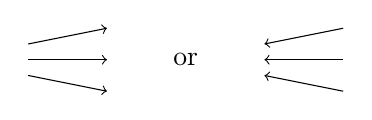
\begin{tikzpicture}
    \draw [->] (0, 0) -- (1, 0);
    \draw [->] (0, 0.2) -- (1, 0.4);
    \draw [->] (0, -0.2) -- (1, -0.4);

    \node at (2, 0) {or};
    \draw [<-] (3, 0) -- (4, 0);
    \draw [<-] (3, 0.2) -- (4, 0.4);
    \draw [<-] (3, -0.2) -- (4, -0.4);

  \end{tikzpicture}
\end{center}
In these cases, We have a force acting to the right for $\zeta > 0$, and to the left if $\zeta < 0$.

These new terms give spontaneous flow, symmetric breaking and macroscopic fluxes. At high $w, \zeta$, we get chaos and turbulence.
\subsubsection*{Active nematic liquid crystals}
In the nematic case, there is no self-advection. So we can't make a velocity from $Q$. We again have
\[
  \frac{\D Q}{\D t} = - \Gamma H,\quad
  H = \left[\frac{\delta F}{\delta Q}\right]^{\text{traceless}}.
\]
where $\frac{\D Q}{\D t}$ is given by
\[
  \frac{\D Q}{\D t} = (\partial_t + \mathbf{v} \cdot \nabla) Q + S(Q, K, \xi).
\]
Here $K = \nabla v$ and
\[
  S = (-\Omega \cdot Q - Q \cdot \Omega) - \xi (D \cdot Q + Q \cdot D) + 2 \xi \left(Q + \frac{1}{d}\right) \Tr(Q \cdot K)
\]
Since there is no directionality as in the previous case, the material derivative will remain unchanged with active matter. Thus, at lowest order, all the self-propelled motion can do is to introduce an active stress term. The leading-order stress is
\[
  \Sigma^A = \zeta Q.
\]
This breaks the free energy structure. Indeed, if we have a uniform nematic, then the passive stress vanishes, because there is no elastic distortion at all. However, the active stress does not since $\zeta Q \not= 0$. Physically, the non-zero stress is due to the fact that the rods tend to generate local flow fields around themselves to propel motion, and these remain even in a uniform phase.

After introducing this, the effective body force density is
\[
  \mathbf{f} = \nabla \cdot \Sigma^A = \zeta \nabla \cdot Q \sim \zeta \lambda (\nabla \cdot \mathbf{n}) \mathbf{n}.
\]
This is essentially the same as the case of the polar case. Thus, if we see something like
\begin{center}
  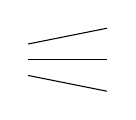
\begin{tikzpicture}
    \draw (0, 0) -- (1, 0);
    \draw (0, 0.2) -- (1, 0.4);
    \draw (0, -0.2) -- (1, -0.4);
  \end{tikzpicture}
\end{center}
then we have a rightward force if $\zeta > 0$ and leftward force if $\zeta < 0$.

This has important physical consequences. If we start with a uniform phase, then we expect random noise to exist, and then the active stress will destablize the system. For example, if we start with
\begin{center}
  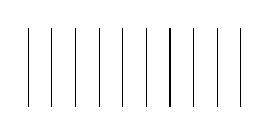
\begin{tikzpicture}
    \foreach \x in {0,0.3,...,3.0}{
      \draw (\x, 0) -- (\x, 1);
    }
  \end{tikzpicture}
\end{center}
and a local deformation happens:
\begin{center}
  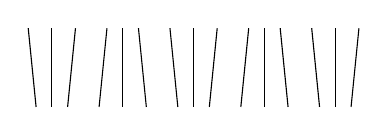
\begin{tikzpicture}
    \foreach \x in {0,1.8,3.6}{
      \draw (\x-0.2, 0) -- (\x - 0.3, 1);
      \draw (\x, 0) -- (\x, 1);
      \draw (\x+0.2, 0) -- (\x + 0.3, 1);
    }
    \foreach \x in {0.9,2.7}{
      \draw (\x-0.2, 1) -- (\x - 0.3, 0);
      \draw (\x, 0) -- (\x, 1);
      \draw (\x+0.2, 1) -- (\x + 0.3, 0);
    }
  \end{tikzpicture}
\end{center}
then in the $\zeta > 0$ case, this will just fall apart. Conversely, bends are destabilized for $\zeta < 0$. Either case, there is a tendency for these things to be destabilized, and a consequence is that active nematics are never stably uniform for large systems. Typically, we get spontaneous flow.

To understand this more, we can explicitly describe how the activity parameter $\zeta$ affects the local flow patterns. Typically, we have the following two cases:
\begin{center}
  \begin{tikzpicture}
    \draw (-0.2, 1) -- (-0.2, 0) arc(180:360:0.2 and 0.05) -- (0.2, 1);
    \draw (0, 1) ellipse (0.2 and 0.05);
    \draw [densely dashed] (-0.2, 0) arc(180:0:0.2 and 0.05);

    \draw [decoration={markings, mark=at position 0.4 with {\arrowreversed[scale=1.2]{latex'}}}, postaction={decorate}] (0.3, -0.3) .. controls (0.3, -0.1) and (0.4, 0.3) .. (0.8, 0.3);
    \draw [decoration={markings, mark=at position 0.4 with {\arrowreversed[scale=1.2]{latex'}}}, postaction={decorate}] (-0.3, -0.3) .. controls (-0.3, -0.1) and (-0.4, 0.3) .. (-0.8, 0.3);
    \draw [decoration={markings, mark=at position 0.4 with {\arrowreversed[scale=1.2]{latex'}}}, postaction={decorate}] (-0.3, 1.3) .. controls (-0.3, 1.1) and (-0.4, 0.7) .. (-0.8, 0.7);
    \draw [decoration={markings, mark=at position 0.4 with {\arrowreversed[scale=1.2]{latex'}}}, postaction={decorate}] (0.3, 1.3) .. controls (0.3, 1.1) and (0.4, 0.7) .. (0.8, 0.7);

    \node at (0, -1) {$\zeta > 0$};
    \node at (0, -1.4) {contractile};
    \begin{scope}[shift={(3, 0)}]
      \draw (-0.2, 1) -- (-0.2, 0) arc(180:360:0.2 and 0.05) -- (0.2, 1);
      \draw (0, 1) ellipse (0.2 and 0.05);
      \draw [densely dashed] (-0.2, 0) arc(180:0:0.2 and 0.05);

      \draw [decoration={markings, mark=at position 0.6 with {\arrow[scale=1.2]{latex'}}}, postaction={decorate}] (0.3, -0.3) .. controls (0.3, -0.1) and (0.4, 0.3) .. (0.8, 0.3);
      \draw [decoration={markings, mark=at position 0.6 with {\arrow[scale=1.2]{latex'}}}, postaction={decorate}] (-0.3, -0.3) .. controls (-0.3, -0.1) and (-0.4, 0.3) .. (-0.8, 0.3);
      \draw [decoration={markings, mark=at position 0.6 with {\arrow[scale=1.2]{latex'}}}, postaction={decorate}] (-0.3, 1.3) .. controls (-0.3, 1.1) and (-0.4, 0.7) .. (-0.8, 0.7);
      \draw [decoration={markings, mark=at position 0.6 with {\arrow[scale=1.2]{latex'}}}, postaction={decorate}] (0.3, 1.3) .. controls (0.3, 1.1) and (0.4, 0.7) .. (0.8, 0.7);

      \node at (0, -1) {$\zeta < 0$};
      \node at (0, -1.4) {extensile};
    \end{scope}
  \end{tikzpicture}
\end{center}
Suppose we take an active liquid crystal and put it in a shear flow. A rod-like object tends to align along the extension axis, at a $45^\circ$ angle.

\begin{center}
  \begin{tikzpicture}
    \begin{scope}[rotate=-45]
      \draw (-0.2, 0.5) -- (-0.2, -0.5) arc(180:360:0.2 and 0.05) -- (0.2, 0.5);
      \draw (0, 0.5) ellipse (0.2 and 0.05);
      \draw [densely dashed] (-0.2, -0.5) arc(180:0:0.2 and 0.05);
    \end{scope}

    \draw [->] (1, -1) -- (-1, -1);
    \draw [<-] (1, 1) -- (-1, 1);

  \end{tikzpicture}
\end{center}

If the liquid crystal is active, then we expect the local flows to interact with the shear flow. Suppose the shear rate is $v_x = y g$. Then the viscous stress is
\[
  \Sigma^\eta = \eta g
  \begin{pmatrix}
    0 & 1\\
    1 & 0
  \end{pmatrix}.
\]
We have
\[
  \Sigma^A \propto \zeta \lambda \left(\mathbf{n}\mathbf{n} - \frac{\mathbf{1}}{d}\right) = \zeta \lambda
  \begin{pmatrix}
    0 & 1\\
    1 & 0
  \end{pmatrix}
\]
if $\mathbf{n}$ is at $45^\circ$ exactly. Note that the sign of $\zeta$ affects whether it reinforces or weakens the stress.

A crucial property is that $\Sigma^A$ does not depend on the shear rate. So in the contractile case, the total stress looks like
\begin{center}
  \begin{tikzpicture}
    \draw [->] (-3, 0) -- (3, 0) node [right] {$g$};
    \draw [->] (0, -2) -- (0, 2) node [above] {$\Sigma_{\mathrm{TOT}}$};

    \draw [mblue, thick] (-3, -1.5) -- (0, -1) -- (0, 1) -- (3, 1.5);
  \end{tikzpicture}
\end{center}
In the extensile case, however, we have
\begin{center}
  \begin{tikzpicture}
    \draw [->] (-3, 0) -- (3, 0) node [right] {$g$};
    \draw [->] (0, -2) -- (0, 2) node [above] {$\Sigma_{\mathrm{TOT}}$};

    \draw [mblue, thick] (-3, -0.5) -- (0, 1) -- (0, -1) -- (3, 0.5); % insert intercepts $\pm g^*$

    \node [circ] at (2, 0) {};
    \node [below] at (2, 0) {$g^*$};
  \end{tikzpicture}
\end{center}

This is very weird, and leads to spontaneous flow \emph{at zero applied stress} of the form
\begin{center}
  \begin{tikzpicture}
    \draw (-2, -1) -- (2, -1);
    \draw (-2, 1) -- (2, 1);

    \draw (-0.5, -1) -- (0.5, 0) -- (-0.5, 1);

    \foreach \y in {0.1,0.3,...,0.9} {
      \draw [-latex](-0.5, 1-\y) -- (-0.5 + \y, 1-\y);
      \draw [-latex](-0.5, \y-1) -- (-0.5 + \y, \y-1);
    }
  \end{tikzpicture}
\end{center}
%The consequence is that at zero applied stress, we want to have bits at $-g^*$ and bits at $g^*$. This gives rise to a spontaneous flow of the form

\subsubsection*{Defect motion in active nematics}
For simplicity, work in two dimensions. We have two simple defects as before
\begin{center}
  \begin{tikzpicture}[scale=0.5]
    \node [circ] {};
    \draw [mblue, semithick, loosely dashed] (-1.732, -0.8) edge [bend right] (-0.2, 2);
    \draw [mblue, semithick, loosely dashed] (-1.732, -0.3) edge [bend right] (-0.7, 2);
    \draw [mblue, semithick, loosely dashed, rotate=120] (-1.732, -0.8) edge [bend right] (-0.2, 2);
    \draw [mblue, semithick, loosely dashed, rotate=120] (-1.732, -0.3) edge [bend right] (-0.7, 2);
    \draw [mblue, semithick, loosely dashed, rotate=240] (-1.732, -0.8) edge [bend right] (-0.2, 2);
    \draw [mblue, semithick, loosely dashed, rotate=240] (-1.732, -0.3) edge [bend right] (-0.7, 2);

    \node [below] at (0, -1.8) {$q = -\frac{1}{2}$};
    \begin{scope}[shift={(6, 0)}]
      \node [circ] {};

      \draw [mblue, semithick, loosely dashed] (0, 0) -- (0, 2);

      \draw [mblue, semithick, loosely dashed] (-0.5, 2) -- (-0.5, 0) arc (180:360:0.5) -- (0.5, 2);
      \draw [mblue, semithick, loosely dashed] (-1, 2) -- (-1, 0) arc (180:360:1) -- (1, 2);
      \draw [mblue, semithick, loosely dashed] (-1.5, 2) -- (-1.5, 0) arc (180:360:1.5) -- (1.5, 2);
      \node [below] at (0, -1.8) {$q = +\frac{1}{2}$};
    \end{scope}
  \end{tikzpicture}
\end{center}
Note that the $q = -\frac{1}{2}$ charge is symmetric, and so by symmetry, there cannot be a net body stress. However, in the $q = +\frac{1}{2}$ defect, we have a non-zero effective force density.

So the defects themselves are like quasi-particles that are themselves active. We see that contractile rods move in the direction of the opening, and the extensile goes in the other direction. The outcome of this is self-sustaining ``turbulent'' motion, with defect pairs $\pm \frac{1}{2}$ are formed \emph{locally}. The $-\frac{1}{2}$ stay put and the $+\frac{1}{2}$ ones self-propel, and depending on exactly how the defect pairs are formed, the $+\frac{1}{2}$ defect will fly away.

Experimental movies of these can be found in \emph{T. Sanchez Nature 491, 431 (2012)}. There are also simulations in \emph{T. Shendek, et al, Soft Matter 13, 3853 (2017)}.

\printindex
\end{document}
